\documentclass[12pt, twoside]{article}
\linespread{1.15}
\usepackage[utf8]{inputenc}  % Ensure this is loaded before biblatex
\usepackage[sorting=none]{biblatex}  % Load the biblatex package
\addbibresource{./../Quellen/sources.bib}  % Add your .bib file


%%%%%%%%%%%%%%%%%%%%%%%%%%%%% Using Packages %%%%%%%%%%%%%%%%%%%%%%%%%%%%%%%%%%
\usepackage[a4paper, margin=2cm, top=5mm, includehead, headheight=2cm]{geometry}
\usepackage{graphicx}
\usepackage{amssymb}
\usepackage{amsmath}
\usepackage{amsthm}
\usepackage{empheq}
\usepackage{mdframed}
\usepackage{booktabs}
\usepackage{lipsum}
\usepackage{graphicx}
\usepackage{color}
\usepackage{psfrag}
\usepackage{pgfplots}
\usepackage{bm}
\usepackage{float}
\usepackage{wrapfig}
\usepackage{enumitem}
\usepackage[export]{adjustbox} % for valign option
\usepackage{caption}
\usepackage{subcaption}
\usepackage{hyperref}
\usepackage{array}
\usepackage{tocloft}
\usepackage[section]{placeins}
\usepackage[nottoc,numbib]{tocbibind}
\usepackage{ragged2e}
\usepackage{pdfpages}
\usepackage[autostyle=true,german=quotes]{csquotes}
\usepackage{siunitx}
\sisetup{locale = DE} 
\usepackage{emptypage}
\usepackage{fancyhdr}
\usepackage{booktabs}
\usepackage{tabularx}
\usepackage{array}
\usepackage{longtable}
\usepackage{multirow}


\usepackage{helvet}

\renewcommand{\familydefault}{\sfdefault}

\renewcommand{\footrulewidth}{0.4pt}%
\renewcommand{\headrulewidth}{0.4pt}%

\renewcommand{\headruleskip}{3mm}
\renewcommand{\footruleskip}{4mm}

\usepackage[main = ngerman, english]{babel}
\usepackage[ddmmyyyy]{datetime}

\newcommand{\todayD}{\the\day.\the\month.\the\year}   

\graphicspath{{../Bilder/}}

\setlength\parindent{0pt}
\counterwithin{figure}{section}
\counterwithin{table}{section}


\clubpenalty=10000
\widowpenalty=10000
\displaywidowpenalty=10000

\let\oldsection\paragraph
\renewcommand{\paragraph}[1]{\needspace{3\baselineskip}\oldsection{#1}}
%%%%%%%%%%%%%%%%%%%%%%%%%%%%%%%%%%%%%%%%%%%%%%%%%%%%%%%%%%%%%%%%%%%%%%%%%%%%%%%
\newcommand{\uni}[1]{\ensuremath{\, \mathrm{#1}}}
\DeclareSIUnit{\Umdrehung}{U}
% Other Settings
\usepackage[dvipsnames]{xcolor}

%\pagecolor[rgb]{0,0,0} %black

%\color[rgb]{0.5,0.5,0.5} %grey

%uncomment to make the links not display the red border
\hypersetup{
    colorlinks,
    citecolor=black,
    filecolor=black,
    linkcolor=black,
    urlcolor=black
}

\sisetup{
detect-all
}


%% codestuff
\usepackage{listings, listings-rust}
\setlength{\parindent}{8pt}
\usepackage{indentfirst}
\definecolor{codegreen}{rgb}{0,0.6,0}
\definecolor{codegray}{rgb}{0.5,0.5,0.5}
\definecolor{codecomment}{rgb}{0.6,0.6,0.6}
\definecolor{backcolour}{rgb}{1,1,1}
\definecolor{lightgray}{rgb}{.9,.9,.9}
\definecolor{darkgray}{rgb}{.4,.4,.4}
\definecolor{codepurple}{rgb}{0.65, 0.12, 0.82}

\lstdefinelanguage{JavaScript}{
    backgroundcolor=\color{backcolour},   
    keywords={typeof, new, true, false, catch, function, return, null, catch, switch, var, if, in, while, do, else, case, break},
    keywordstyle=\color{NavyBlue},
    ndkeywords={class, export, boolean, throw, implements, import, this},
    ndkeywordstyle=\color{codegray},
    identifierstyle=\color{black},
    sensitive=false,
    comment=[l]{//},
    morecomment=[s]{/*}{*/},
    commentstyle=\color{codecomment},
    stringstyle=\color{codepurple}\ttfamily,
    morestring=[b]',
    morestring=[b]"
}

\lstdefinestyle{mystyle}{
    basicstyle=\fontsize{10}{12},
    backgroundcolor=\color{backcolour},   
    commentstyle=\color{codecomment},
    keywordstyle=\color{NavyBlue},
    numberstyle=\tiny\color{codegray},
    stringstyle=\color{codepurple},
    basicstyle=\ttfamily\footnotesize\bfseries,
    breakatwhitespace=false,         
    breaklines=true,                 
    captionpos=t,                    
    keepspaces=true,                 
    numbers=left,
    numbersep=5pt,                  
    showspaces=false,                
    showstringspaces=false,
    showtabs=false,                  
    tabsize=2
}
% -- Setting up the custom style:
\lstset{style=mystyle}

%%%%%%%%%%%%%%%%%%%%%%%%%% Page Setting %%%%%%%%%%%%%%%%%%%%%%%%%%%%%%%%%%%%%%%
\geometry{a4paper}

\newcommand{\iu}{{i\mkern1mu}}
\newcommand*\mathinhead[2]{\texorpdfstring{$\boldsymbol{#1}$}{#2}}

\definecolor{mred}{rgb}{0.619, 0.2392, 0.3176}


%%%%%%%%%%%%%%%%%%%%%%%%%%%%%%% Title & Author %%%%%%%%%%%%%%%%%%%%%%%%%%%%%%%%
\title{AFSS - Automated Factory Storage System}
\author{Benedikt Simbürger \\
    \and Nikolaj Voglauer \\
    \and Vincent Sonvilla \\
    \and Elena Widmann
    }

%%%%%%%%%%%%%%%%%%%%%%%%%%%%%%%%%%%%%%%%%%%%%%%%%%%%%%%%%%%%%%%%%%%%%%%%%%%%%%%
\babelprovide[import]{ngerman}


\fancyhf{}

\fancyhf[EHL]{\includegraphics[width=0.2\textwidth]{HTL_Moessingerstraßen_Logo.png}}
\fancyhf[OHL]{\includegraphics[width=0.2\textwidth]{HTL_Moessingerstraßen_Logo.png}}

\fancyhf[EHC]{\begin{tabular}{cc}
    Simbürger & Sonvilla \\
    Voglauer & Widmann \\
\end{tabular}}

\fancyhf[OHC]{\begin{tabular}{cc}
    Simbürger & Sonvilla \\
    Voglauer & Widmann\\
\end{tabular}}


\fancyhf[EFL]{\todayD}
\fancyhf[EFR]{\thepage}
\fancyhf[EHR]{\color{mred} ELEKTROTECHNIK}


\fancyhf[OFR]{\todayD}
\fancyhf[OFL]{\thepage}
\fancyhf[OHR]{\color{mred} ELEKTROTECHNIK}

\fancyhf[EFC]{Automated-Factory-Storage-System}
\fancyhf[OFC]{Automated-Factory-Storage-System}

\raggedbottom

\begin{document}

\pagenumbering{gobble}

\setlength{\parindent}{0pt}

\begin{figure}[h]
    \vspace{-5mm}
    \includegraphics[width=0.5\textwidth]{HTL_Moessingerstraßen_Logo.png}
    \centering
\end{figure}

\begin{center}
    \Large \textbf{HÖHERE TECHNISCHE BUNDESLEHRANSTALT} \\
    \vspace{5mm}
    \Large{KLAGENFURT, MÖSSINGERSTRASSE}

\end{center}

\vspace{7mm}

\begin{center}
    \Large{ABTEILUNG ELEKTROTECHNIK}
\end{center}

\hrule

\vspace{10mm}

\begin{center}
    \Huge \textbf{DIPLOMARBEIT} \\
    \vspace{7mm}
    \huge{Titel der Diplomarbeit Deutsch}

    \vspace{7mm}
    \huge{Automated-Factory-Storage-System}

    \vspace{7mm}
    \Large{JAHRGANG 5AHET}

\end{center}

\vspace{15mm}

\begin{flushleft}
    \linespread{1}
    \bgroup
        \large
        \def\arraystretch{1.5}
        \begin{tabular}{p{5cm}l}
            eingereicht von & Benedikt Simbürger\\
            & Vincent Sonvilla\\
            & Nikolaj Voglauer\\
            & Elena Widmann\\
            Projektbetreuer & Dipl.-Ing. Christian Sallinger
        \end{tabular}
    \egroup
\end{flushleft}

\vspace{7mm}
\large
Diese Diplomarbeit entspricht den Standards gemäß dem Leitfaden zur Umsetzung der Reife- und Diplomprüfung des BMBWF in der letztgültigen Fassung.\par
\begin{flushright}
    Klagenfurt, am 04.04.2025
\end{flushright}

\newpage

\begin{figure}[h]
    \includegraphics[width=0.5\textwidth]{HTL_Moessingerstraßen_Logo.png}
    \centering
\end{figure}

\begin{center}
    \huge \textbf{EIDESSTATTLICHE ERKLÄRUNG}\\
    \vspace{7mm}
    \large
    \begin{tabular}{p{14cm}}
        Ich versichere an Eides statt, dass ich diese Diplomarbeit
        selbstständig verfasst und keine anderen als die angegebenen
        Quellen und Hilfsmittel verwendet habe. Alle Gedanken, die im
        Wortlaut oder in grundlegenden Inhalten aus unveröffentlichten
        Texten oder aus veröffentlichter Literatur übernommen, oder mit
        künstlicher Intelligenz generiert wurden, sind ordnungsgemäß
        gekennzeichnet, zitiert und mit genauer Quellenangabe
        versehen.
    \end{tabular}

    \vspace{10mm}
    Verfasser/Verfasserin\\
    
    \vspace{40mm}
    \bgroup
        \newcolumntype{P}[1]{>{\centering\arraybackslash}p{#1}}
        \def\arraystretch{1.5}
        \begin{tabular}{P{67mm}p{14mm}P{67mm}}
            \cline{1-1}
            \cline{3-3}
            Benedikt Simbürger & & Vincent Sonvilla\\
        \end{tabular}

        \vspace{35mm}
        \begin{tabular}{P{67mm}p{14mm}P{67mm}}
            \cline{1-1}
            \cline{3-3}
            Nikolaj Voglauer & & Elena Widmann\\
        \end{tabular}
    \egroup

    \vspace*{\fill}
    \raggedleft Klagenfurt, am 04.04.2025

\end{center}

\newpage

\pagestyle{fancy}
\pagenumbering{arabic}
\normalsize

\section*{Kurzbeschreibung}

Das Bauteillager der Werkstätte der HTL-Mössingerstraße ist aktuell eine Kombination aus Schränken und Fächern, bei denen von Hand ein- und ausgelagert werden muss. Da dies sehr zeitaufwendig und fehleranfällig ist, soll eine automatische Lösung Abhilfe schaffen. \\

Ziel des Projekts "Automated-Factory-Storage-System" ist es, eine Gesamtlösung für ein automatisches Kleinteillagersystem nach dem Vorbild der Industrie zu entwickeln. So soll unter anderem ein Realitätsbezug zu dem im Unterricht Gelernten geschaffen werden. Deshalb werden auch alle Steuerungskomponenten so industrienah wie möglich ausgeführt. Außerdem wird es möglichst erweiterbar ausgeführt, um zukünftige Erweiterungen zu ermöglichen.\\

Die Mechanik besteht aus einem eigens entwickelten Miniatur-Hochregallager, welches ähnlich eines Palettenlagersystems Boxen aus einem Regal mit rund 200 Lagerplätzen ein- und ausheben kann. Über einen Querförderer werden die Boxen auf ein Förderband gebracht und können dann zu einer Kommissionierstation gefahren werden. Als Grundlage wird hier auf Aluminiumprofilsysteme zurückgegriffen. Die Aktorik besteht aus Schrittmotoren.\\

Zur Steuerung wird ein Serverschrank zu einem Schaltschrank umgebaut, welcher alle Sicherungs- und Steuerungskomponenten beinhaltet. Alle Verbindungen zwischen Schaltschrank und Mechanik sind außerdem leicht absteckbar, und das Lager sowie der Schaltschrank sind mobil, um diese leicht transportieren zu können.\\

Die Ansteuerung erfolgt über eine SPS. Diese steuert die Schrittmotoren und verarbeitet die Sensorsignale. Diese bestehen aus Referenz- und Endschaltersignalen für alle Achsen und werden über einen Feldbus zusammengefasst. \\

Die SPS kommuniziert dann mit einer selbst programmierten Lagerverwaltungssoftware, welche den Lagerbestand verwaltet und eine Benutzeroberfläche bietet. Den Benutzenden ist es hier möglich, Artikel zu bestellen und den Lagerbestand zu ändern.\\

Außerdem werden die Mechanik sowie die Elektrik so ausgelegt, dass ein möglichst sicherer Betrieb möglich ist, um sowohl Mensch als auch Maschine nicht zu schaden.
\\\\
\bgroup
    \def\arraystretch{1.5}
    \begin{tabular}{p{48mm}p{113mm}}
        \textbf{Kurztitel:} & Automated-Factory-Storage-System\\
        \textbf{Schlüsselwörter:} & Hochregallager, Lagerverwaltung, Schaltschrankbau, SPS-Programmierung
    \end{tabular}
\egroup

\newpage

\section*{Short Description}

The component storage of the HTL-Mössingerstraße workshop is currently a combination of cabinets and compartments, where storage and retrieval must be done manually. Since this process is very time-consuming and error-prone, an automated solution is intended to provide relief. \\

The goal of the "Automated-Factory-Storage-System" project is to develop a complete solution for an automated small-parts storage system modeled on industrial standards. This will help create a practical reference to the knowledge learned in class. Therefore, all control components will be implemented as industry-oriented as possible. Additionally, the system will be designed to be modular to allow future expansions.\\

The mechanical system consists of a custom-developed miniature high-bay storage system that, similar to a pallet racking system, can lift and store boxes from a rack with approximately 200 storage spaces. A transverse conveyor transports the boxes onto a conveyor belt, which can then move them to a picking station. The system is based on aluminum profile structures. The actuators consist of stepper motors.\\

For control, a server cabinet will be converted into a control cabinet, which will house all safety and control components. All connections between the control cabinet and the mechanical system are easily detachable. Both the storage system and the control cabinet are mobile to ensure easy transport.\\

The control system operates via a PLC. This PLC controls the stepper motors and processes sensor signals. These signals consist of reference and limit switch signals for all axes and are consolidated via a fieldbus. \\

The PLC then communicates with a self-developed warehouse management software that manages inventory and provides a user interface. Users can place orders and modify inventory levels.\\

Furthermore, the mechanical and electrical systems are designed to ensure the highest possible level of safety to protect both humans and machines.
\\\\
\bgroup
    \def\arraystretch{1.5}
    \begin{tabular}{p{48mm}p{113mm}}
        \textbf{Short Title:} & Automated-Factory-Storage-System\\
        \textbf{Keywords:} & High-bay warehouse, warehouse management, control cabinet construction, PLC programming
    \end{tabular}
\egroup



\newpage

\tableofcontents
\newpage
\section{Allgemeiner Teil}

\subsection{Ausgangssituation}
Die HTL-Mössingerstraße arbeitet im Zuge der Werkstätte mit einer Factory, diese ist eine Miniatur-Firma bei der Lehrpersonal sowie SchülerInnen Bestellungen abgeben können. Diese Bestellungen werden dann von zugeteilten SchülerInnen abgearbeitet.\\
In dieser Factory laufen die Bestellprozesse digital über eine schulinterne Website. Verwendet werden von der Factory 3D-Drucker, CNC-Fräsen, Lasercutter und diverse weitere Maschinen, um Angefordertes zu produzieren. Die Factory stellt primär Einzelteile zur Verfügung, dazu gehört auch ein großes Repertoire an Bauteilen, die im Lager der Factory gelagert werden.\\ 
Die Handhabung dieses Lagers erfolgt bisher manuell. SchülerInnen schreiben in einer digitalen Applikation mit, welche Teile ein- bzw. ausgelagert werden. SchülerInnen sind im Schnitt nur ein Schuljahr in der Factory. In dieser Zeitspanne ist es kaum möglich eine Routine einzuarbeiten und die Fehlerquote bei der Arbeit im Lager ist relativ hoch. Das führt zu fehlerhaften Lieferungen oder verzögerten Produktionsketten.\\
Ein weiterer Nachteil des derzeitigen Lagers ist, die Örtlichkeit. Das Lager befindet sich zurzeit im Keller und ist dort fest verbaut. Die schweren Schränke und Regale können im Falle von Hochwasser, wie im Sommer 2023, weder schnell ausgelagert oder verschoben werden.\\ 
Im Allgemeinen Schulgeschehen ergeben sich zudem Möglichkeiten der Migration fürs Lager, um Prozesswege der Factory effizienter zu gestalten. Mit dem derzeitigen Lager können keine potenziellen Optionen wahrgenommen werden. 

\subsubsection{Anforderungen}

Um die Automatisierung dieses Prozesses zu ermöglichen, soll ein System entwickelt und gebaut werden, das eine lagernde Box automatisch zu einer Kommissionierstation bringt. An dieser Station soll die Möglichkeit bestehen, Inventar anzufordern, Lagerbestände auszugeben oder aufzufüllen sowie Boxen wieder einzulagern.
\\
Weiterhin muss dieses System erweiterbar sein, um zukünftig zusätzlichen Lagerplatz hinzuzufügen und die Integration anderer Systeme, wie beispielsweise einer Bauteilvereinzelung, zu ermöglichen.
\\
Zudem soll das AFSS mobil sein – sowohl mechanisch als auch elektrisch –, da es nicht am endgültigen Standort errichtet wird und einen einfachen Transport bei möglichen Umbauarbeiten ermöglichen soll.
\\
Die Rahmenbedingungen für die Umsetzung dieser Ziele sind stark davon geprägt, dass alle mechanischen Bauteile, die eigens gefertigt werden müssen, so konstruiert werden, dass ihre Herstellung mit den Mitteln der HTL möglich ist.
\\
Das System soll nicht nur produzierbar, sondern auch reproduzierbar sein. Daher muss die Dokumentation der Funktion sowie des Umsetzungsprozesses so erfolgen, dass das Projekt von nachfolgenden Schüler*innen weitergeführt werden kann.



\subsection{Potentielle Lösungen}
\subsubsection{Lagermethoden}
Die Industrie bietet viele Vorbilder dafür, wie ein boxenbasiertes Lagersystem aufgebaut sein kann.
\\
Eine besonders platzeffiziente Variante ist beispielsweise die PickEngine von KNAPP \cite{pickengine}. Bei dieser Lösung werden Boxen in mehreren Ebenen übereinander gelagert. Auf jeder Ebene gibt es bewegliche Roboter, die die Boxen abholen und zu einem Lift bringen, von dem aus die Box dann zur Kommissionierstation transportiert wird. Dieses System ist sowohl platzsparend als auch sehr ausfallsicher. Allerdings ist es schwierig, ein solches System in Miniatur nachzubauen, da die Hardwarefertigung sehr komplex ist.
\\
Eine weitere Möglichkeit wäre ein rotierendes Magazin, in dem die Boxen auf einem horizontalen Karussell gelagert sind. Wenn ein bestimmtes Produkt benötigt wird, rotiert das Karussell so lange weiter, bis die gewünschte Box zugänglich ist. Das Prinzip dieses Systems ist zwar recht simpel, jedoch stellt die mechanische Umsetzung der Rotation mit den Mitteln der HTL eine Herausforderung dar, insbesondere im Hinblick auf einen zuverlässigen Dauerbetrieb.
\\
Eine dritte Option besteht darin, die Ware vertikal von oben zu lagern. Über der Lagerstätte bewegt sich ein Roboter, der die Boxen ausheben, umschichten sowie ein- und auslagern kann. Dieses System ermöglicht eine hohe Lagerdichte, hat jedoch den Nachteil eines begrenzten Durchsatzes. Wenn eine Box benötigt wird, die nicht an oberster Stelle liegt, müssen erst alle darüberliegenden Boxen umgeschichtet werden. Zudem ist diese Lagervariante erst dann wirklich platzsparend, wenn sie sehr hoch gebaut wird. Bei wenigen Ebenen lohnt sie sich noch nicht, da trotz geringer Höhe bereits viel Fläche verbraucht wird.



\subsubsection{Steuerung (bitte keine vergangenheitsformen)4/9}
Es gibt durchaus verschiedenste Methoden zur Steuerung von Anlagen. Bekannterweise werden hier Speicherprogrammierbare Steuerungen, kurz SPS, verwendet. Diese bieten den Vorteil, komplexe Steuerungen durch Programmierung mit intuitiven Programmiersprachen realisieren zu können. Jedoch erfordern SPS für jeden Zusatz, beispielsweise digitale Ein-/Ausgänge oder das Ansteuern von Motoren, verschiedenste Module. \\
Eine günstigere Variante zu Speicherprogrammierbare Steuerungen bieten Arduinos. Diese benötigen aber für das Ansteuern von energielastigeren Bauelementen auch zusätzliche Elemente. Zusätzlich steigt der Programmier-Aufwand, sowie die Komplexität des \textbf{des is schon a bissi hoch gestochen} Programms, bei großen Anlagen ins Unermessliche, da jedweilige Motoransteuerung oder Verbindung mit Servern ausprogrammiert werden muss. Dieser Aufwand wäre in diesem Projekt zeitlich nicht schaffbar.\\
Ein wenig teurer als Arduino, aber noch unter dem Preis einer SPS, liegen Verbindungsprogrammierbare Steuerungen, welche die Funktion dadurch realisieren, wie sie verdrahtet sind, über Relais, Schalter, etc. Diese sind aber mit einem beträchtlichen Aufwand, aufgrund von Verkabelung sowie Anschaffung benötigter Materialien, verbunden. Zusätzlich ist die Realisierung von komplexeren Projekten durchaus zeitintensiv. 


\subsubsection{Schaltschrank}
Für die Elektronik gibt es mehrere Möglichkeiten der Umsetzung. Beleuchtet wurden im Entwicklungsprozess integrierte Bauweisen in das AFSS, neuwertige Schaltschränke sowie Umbaumöglichkeiten.\\
Die erste Idee, die verfolgt wurde, war ein integrierter Schaltschrank im AFSS. Dieser hätte einen Rahmen aus Aluminiumprofilen, Plexiglasscheiben hätten die Komponenten vom Rest getrennt und die einzelnen Elemente wären auf eine gefrästen Aluminiumplatte montiert worden. Vorteil dieser Option ist eine kompakte Bauweise, man hätte keinen zusätzlichen Schrank. Nachteile sind Zusatzkosten, Lagerplatzverluste da das Lager nicht breiter gemacht werden kann und kein Platz für Erweiterungen.\\
Ein neuer Schaltschrank wäre grundsätzlich die naheliegendste  Lösung. Für das AFSS hätte der Schaltschrank groß sein müssen, um alle Komponenten unterzubringen und um die Erweiterbarkeit zu gewährleisten. Vorteilhaft wäre, verminderter Bauaufwand und eine gute el. Sicherheit. Allerdings ist ein herkömmlicher Schaltschrank nicht mobil und ist somit für eine mobile Anlage ungeeignet, zudem entstehen Zusatzkosten.\\	
Die letzte Option war ein alter Serverschrank, dieser kommt mit vier Profilschienen, einer Lüftungsanlage und war groß genug, um die Anforderung der Erweiterbarkeit auch zu erfüllen. Zusätzlich gemacht gehört sind Module, die auf die Schienen montiert werden, auf diesen wären die el. Komponenten montiert. Die Module können aus kosteneffizienten Platten hergestellt werden. Um den Serverschrank mobil zu machen, müssten kleinere Umbauten durchgeführt werden.




\subsection{Verfolgter Lösungsansatz 3/4}

\subsubsection{Lagermethoden }
Nach Abwägung der Alternativen wurde bei der Auswahl der Lagermethode ein klassisches Palettenlager als Inspiration gewählt. Der Grundgedanke basiert auf einem Portalsystem, das mit einer Gabel Boxen in einem Regal ein- und aushebt. Diese Lagervariante vereint die Balance aus technischer Komplexität und dem Umsetzungsvermögen an der HTL. Zudem gibt es bei dieser Variante ebenfalls Potenzial zur Effizienzsteigerung, da die Möglichkeit besteht, links und rechts des Roboters Bestand zu lagern. Allerdings wird diese Variante nicht forciert, da die Komplexität eines solchen Mechanismus im kleinen Maßstab und mit eingeschränkter Fertigungstechnik recht schwierig umzusetzen ist.
\\
Es wurde also ein Lagersystem gewählt, bei dem zwei Achsen hin- und herfahren und eine Art Gabel die Boxen ein- und aushebt. Um die Boxen zur Kommissionierstation zu bringen, wird ein Förderband verwendet, das längs zum Lager verläuft. Der Lagerroboter kann die Boxen jedoch nicht selbstständig auf das Förderband laden. Zu diesem Zweck wird ein sogenannter Querförderer eingesetzt, der die Box von einem temporären Lagerplatz auf das Förderband und wieder zurück schiebt. An dieses Förderband können außerdem weitere solcher Lagerschränke angeschlossen werden, um mehr Lagerplatz zu schaffen und auch andere Systeme anzubinden. Darüber hinaus wird ein Lagerschrank als Komplettsystem konzipiert. Durch die Unterbringung aller Systeme in einem einzigen Objekt kann die Transportfähigkeit durch die Montage von Rollen einfach sichergestellt werden.

\subsubsection{Steuerung 1/4}
Als Steuerung wurde eine SPS von Siemens ausgewählt, da das Basic Know-How für die Programmierung solcher, bereits in der Schule gelehrt wird. Zudem sind speicherprogrammierbare Steuerungen ideal für komplexere Anlagen und ermöglichen die Ansteuerung der Motoren sowie die Kommunikation mit dem Server relativ simpel und bleiben dabei auch innerhalb der geforderten Zykluszeit. 

\subsubsection{Schaltschrank 1/4}
Der Umbau vom Serverschrank war die beste Option. Es wird Altbestand verwertet, es ist eine kosteneffiziente Lösung die viel Freiheit zur Anpassung an spezielle Komponenten erlaubt. Zudem gibt es viel Platz für Erweiterungen und Räder an den Schrank zu montieren wäre kein großer Zusatzaufwand. Die elektrische Steuerung der Anlage, die Versogungsgeräte und weiter Elemente finden in diesem Schrank auch platz. Weiters kann mit dieser Option auch erreicht werden, dass der Schaltschrank mittels weniger Handgriffe vollkommen vom Lagerschrank getrennt werden kann.
Eine gute Lösung für die Ansprüche.
\subsection{Methodik 5}

\subsubsection{Software 2}

Zur Dokumentation der elektrischen Komponenten und deren Verbindungen wird E-Plan verwendet. E-Plan ist der Industriestandard und bietet unzählige Möglichkeiten für eine ausführliche Dokumentation. E-Plan hilft ein übersichtliches Schaltbild zu erstellen, und die Anlage lesbar festzuhalten. Auch im Planungsprozess ist E-Plan der Schlüssel zu einer vollständigen Planung.

\paragraph{Fusion360/PCB}\mbox{}\\
Zur mechanischen Planung des AFSS wird vorrangig Fusion360 genutzt. Dies ist ein 3D-CAD (Computer-Aided-Design) Programm, welches eine breite Palette von Funktionen bietet, jedoch noch sehr bedienerfreundlich ist. Weiters ist es sehr nützlich, dass Fusion360 eine integrierte Cloud-Speicherung anbietet. So können die Konstruktionen von anderen Personen einfach eingesehen werden.\\

Die volle Integration von Eagle in Fusion360 im Jahr 2020 macht es möglich, auch in Fusion360 Leiterplatten zu entwerfen und die dazugehörigen Schaltungen zu zeichnen. Der Verkauf des Programms Autodesk Eagle wird mit Juni 2026 eingestellt und ist somit nicht mehr Stand der Technik.\cite{Eagle_in_Fusion} Das Entwerfen von PCBs (Printed Circuit Boards) ist durch die Integration in Fusion360 nicht nur einfacher, sondern auch einheitlicher geworden. Außerdem kann durch die Zusammenführung der beiden Programme ermöglicht werden, dass Projekte auf einer zentralen Entwurfsplattform umgesetzt werden.

\paragraph{AutoCAD}\mbox{}\\
Zur mechanischen Planung des AFSS wird auch AutoCAD verwendet. Vor allem für Pläne von Frästeilen oder Laserteilen bietet sich diese Applikation an. AutoCAD wird in der Industrie verwendet und bietet eine benutzerfreundliche Oberfläche sowie eine breite Palette an Funktionen.


\paragraph{Lagerverwaltungssoftware}\mbox{}\\
Um Lagerbestand zu verwalten bedarf es eines ausgeklügelten Systems, welches einerseits eine Benutzerbedinenung zulässt, und andererseits die Logik der Auslagerung übernimmt. \\
Eine Möglichkeit dies zu Erreichen, wäre eine reine Softwarelösung nur auf SPS-Basis. Dies ist aber sehr sher umständlich und auch nicht skalierbar. Auch die verwendung von graphischen Entwicklungswerkzeugen wie Node-Red wäre denkbar, jedoch ist es auch hier schwierig komplexe Operationen durchzuführen, wenngleich die Einbindung zur SPS einfacher ist.\\
Die Favorisierte Lösungsvariante für dies Anforderungen ist die Entwicklung eines eigenen Servers in einer Programmierhochsprache. Die SPS soll mit diesem Kommunizieren können. Ausserdem kann dieser Server eine Benutzeroberfläche für die Bedienung zur verfügung stellen, sowie die Steuerungslogik übernehmen. Dieser soll überdies auf eine Datenbank zugreifen, welche den Lagerbestand abbildet.


\paragraph{TIA Portal}\mbox{}\\
Ist die Software, welche verwendet wird, um speicherprogrammierbare Steuerungen von Siemens anzusteuern.TIA-Portal bietet die Möglichkeit, in verschiedensten Programmiersprachen zu arbeiten (Funktionsplan (FUP), Kontaktplan (KOP), einer Anweisungsliste (AWL), mit Structered Code Language (SCL) oder Graph.) Zudem können externe Anwendungsspezifische Funktionsbausteine mit Bibliotheken eingebunden werden.
\cite{TIA_Portal_Programmiersprachen}

\subsubsection{Hardware 2}

\paragraph{Antriebe}\mbox{}\\
Das elektrische Antriebssystem ist ein Kernbaustein des AFSS. Mit diesem werden alle beweglichen Aktoren betätigt. Hier ist es nötig, einen Kompromiss zwischen Leistung, Kosten und der Ansteuerbarkeit zu finden.
\\
Industrieservomotoren, die typischerweise mit 400 V, Frequenzumrichtern und Gebern betrieben werden, sind zwar sehr leistungsdicht und gut steuerbar, jedoch auch sehr teuer. Aus diesem Grund wurde schnell ein Antriebssystem aus Closed-Loop- und Open-Loop-Schrittmotoren angestrebt.
\\
Für alle Anwendungen mit hohen Drehmomenten (X- und Y-Achse) sollen Closed-Loop-Schrittmotoren im Formfaktor Nema23 verwendet werden. Diese können im Falle unerwarteter Laständerungen ohne Schrittverlust weiterbetrieben werden und sind zudem in den benötigten Drehmomentbereichen preiswert verfügbar. Jedoch müssen für diese Motoren Treiber eingesetzt werden. Diese verarbeiten die Signale der SPS und treiben den Motor an. Zudem verarbeiten sie auch die Gebersignale. Falls eine Diskrepanz zwischen Gebersignal und Steuersignal erkannt wird, wird dies automatisch ausgeglichen.
\\
Für die Z-Achse (Gabel) sowie für den Querförderer ist lediglich ein Open-Loop (geberloser) Antrieb nötig. Hier werden Nema17 Motoren eingesetzt. Bei diesen Achsen ist es relativ einfach, bei jedem Verfahren die tatsächliche aktuelle Position mit der vermuteten Position zu vergleichen, da jedes Mal über den Referenzierpunkt gefahren wird.

\paragraph{Sensoren}\mbox{}\\
Die Sensoren sind wesentlich für eine sichere und korrekte Funktion des AFSS. Sie werden zur Übermittlung der genauen Positionierung der Achsen eingesetzt, aber auch zum Überprüfen, ob die jeweiligen Boxen an den Zielpositionen angekommen sind.\\
Zur Übertragung des Sensorsignals wird ein AS-i-Bus verwendet. Dieser bietet eine einfache Kommunikation zwischen den Sensoren und der SPS. Die Sensoren werden über den AS-i-Slave mit 24V versorgt, jedoch ist zu beachten, dass vereinzelte Sensoren mit einer niedrigeren Spannung betrieben werden müssen, um eine lange Lebensdauer und korrekte Funktion garantieren zu können.\\
Ohne mechanische Endschalter würde die Gefahr bestehen, dass die Motoren nicht gestoppt werden und der Rahmen angefahren wird, was zu erheblichen Schäden am System führen kann. Aus Verfügbarkeitsgründen  werden an den verschiedenen Achsen unterschiedliche Arten von Sensoren als mechanische Endschalter eingesetzt. Die Achsen werden mittels eines Photo-Interrupters, der auf einer eigens entworfenen Platine untergebracht ist, referenziert. Zum Überprüfen, ob die jeweilige Box ihre Zielposition erreicht hat, werden Lichttaster eingebaut. Zur Zuordnung der Boxen und den sich darin befindenden Bauteile werden auf den Boxen Barcodes angebracht. Um diese einlesen zu können befindet sich auf der Kommissionierstation ein Barcodescanner, der die jeweilige EAN-Nummer an die SPS weitergibt, die diese wiederum an den Server weiterleitet.\\


\paragraph{Elektrik}\mbox{}\\
Die elektrische Seite der Anlage besteht unter anderem aus diesen 7 Schrittmotoren, wobei Drei davon schwächer sind. Wenn alle Motoren gleichzeitig anlaufen können Ströme von gut mehr als 20 A entstehen. deswegen werden die Motoren auf zwei 20 A/24 V Gleichspannungs-Netzteile aufgeteilt. Die Logik an der Anlage besteht aus einer Siemens SPS samt Ein- und Ausgangsmodul sowie zwei PTO-Modulen. Der Logikkreis samt SPS sollen getrennt gespeißt werden, mit einem 24V/10A Gleichspannungsnetzteil-Netzteil. Die Sensoren auf der Anlage laufen über einen ASI-Bus, der Master ist eine Karte für eine ET200. Das ASI-System muss über ein ASI-Netzteil gespeißt werden. Das Fließband wird von einem Asynchronmotor mit 1.1 A Nennstrom betrieben. dieser wird über eine Wendeschützschaltung angesteuert. Die Schütz werden von Relais angesteuert und mit einen Motorschutz wird der Motor \textbf{(vor überlast)} geschützt. Die Anlage wird über einen FI und einen Leitungsschutzschalter abgesichert und hat zudem einen Schlüsselschalter und einen dreiphasigen Drehschalter zur manuellen Freigabe.\\
Die Motoren haben jeweils einen Encoder dabei. Somit müssen ein Motorkabel und ein Kabel für den Encoder verlegt werden. Beide Kabel müssen geschrimt sein. 



\subsubsection{Fertigung 1}

\paragraph{Lasern}\mbox{}\\
An der HTL-Mössingerstraße ist es den SchülerInnen möglich einen Lasercutter zur Kunstoffverarbeitung zu verwenden. Um ein gewünschtes Teil fertigen zu können, muss die Kontour dieses als .dwg zur verfügung stehen. Dieses kann dann unter berücksichtigung der Materialstärke aus verschiedenen Farben geschnitten werden.


\paragraph{Fräsen}\mbox{}\\
Um Aluminiumteile zu fertigen steht eine 3-Achsen CNC-Fräse zur Verfügung. In dieser ist es möglich die Teile zu fräsen, die aufgrund ihrer hohen mechanischen Beanspruchung nicht aus Kunststoff gefertigt werden können, aus anderen Materialien herzustellen. Um dies zu bewerkstelligen, muss zuerst der G-Code in Filou-NC16 programmiert werden und kann dann in NC-Easy auf der CNC-Fräse ausgeführt werden. Da der Fräser jedoch einen größeren Durchmesser als der Laser hat, muss, wenn Ecken benötigt werden, eine Aussparung größer dem Durchmesser des Fräsers, eingeplant werden.\\
Als Aluminiumlegierung wird hier die Legierung EN-AW 5754 (AlMg3) verwendet. Diese Legierung aus Aluminium und Magnesium eignet sich sehr gut zum Fräßen und ist in der Lage, die mechanischen Beanspruchungen auszuhalten.

\paragraph{Aluminium-Extrusionen schneiden}\mbox{}\\
Um Aluminiumextrusionen abzulängen wird eine eigens dafür ausgelegte Kreissäge verwendet. In dieser ist es möglich einen Anschlag für eine bestimmte Länge einzustellen und dann abzuschneiden. Dadurch ist es möglich in kurzer Zeit viele verschiedene Längen präzise zuzuschneiden. 

\paragraph{3D-Drucken}\mbox{}\\
Für die Herstellung von Kunststoffteilen, die im Lasercutter nicht gefertigt werden können, stehen den Schülern mehrere 3D-Drucker zur verfügung. Die Drucker können mit verschiedensten Materialen drucken, beispielsweise PLA oder ABS. Komplexe Bauteile die nicht über die räumlichen Begrenzungen der Drucker hinausgehen, können so gefertigt werden. Dazu wird ein 3D-Modell im stl.-Format benötigt, welches dann in einem Slicerprogramm in G-Code oder Bg-Code umgewandelt werden kann\cite{How_to_PrusaSlicer}. Schulintern wird hierzu primär der PrusaSlicer verwendet.

\subsection{Sicherheitstechnik}
Um eine langjährige korrekte Funktion des AFSS sicherstellen zu können, müssen diverse Sicherheitsvorkehrungen getroffen werden. Diese lassen sich unterteilen in die Sicherheit der Personen, die das Lagersystem bedienen, und in die Sicherheit des Systems selbst, vor Beschädigung durch Fremdeinwirkungen oder im eigenen Fehlerfall. Um die Sicherheitstechnik richtig umsetzen zu können, muss diese bereits im Vorhinein durchdacht und gut geplant werden.\\
Um die Benutzerinnen und Benutzer gegen Verletzungen zu schützen muss das AFSS so positioniert werden, dass diese bei ordnungsgemäßen Gebrauch nicht in Gefahr geraten können. Der Schaltschrank sollte so ausgelegt und abgesichert werden, dass Personen nicht bei normaler Benutzung in Stromkreise geraten oder in Berührung mit unter Spannung stehenden Betriebsmitteln kommen können. Die Sicherheit von Personen hat oberste Priorität und wird über die Sicherheit des Systems gestellt.\\
Ebenfalls müssen die mechanischen sowie elektrischen Elemente so ausgelegt werden, dass Nutzer beim Normalgebrauch des AFSS diesem keine Schäden zufügen können. In den meisten Fällen sorgen die Sicherheitsvorkehrungen, die bereits für die Sicherheit der bedienenden Personen sorgen, auch gleichzeitig für Schutz gegen Fremdeinwirkung. Dazu gehört die Abgrenzung der empfindlichen Mechanik des Lagers durch bewusste Positionierung, sowie eine verschließbare Türe am Schaltschrank, die eine klare Trennung zwischen Elektrik und Nutzer gewährleistet.\\
Damit die Motoren des Lagersystems nicht nur im Normalbetrieb zum Stoppen gebracht werden, sondern im Fehlerfalle auch die Grenzen der jeweiligen Achsen nicht überschreiten und so keine Schäden an der Mechanik anrichten können, werden neben den Software-Endschaltern zusätzliche Hardware-Endschalter eingebaut. Zur Sicherung der Motoren soll ein Überstromschutz eingebaut werden. Der Schaltschrank und die sich darin befindenden Elemente und deren Verkabelung sollen so geplant und verbaut werden, dass es zu keinen Kurzschlüssen, Bränden oder anderen Schäden kommen kann. Sollte es dennoch zu einer Situation kommen, in der das AFSS sofort zu einem Stopp gebracht werden muss, werden zum Anhalten des gesamten Systems leicht sicht- und erreichbare Not-Aus-Taster verbaut.

\subsection{Kooperationspartner 2X weety, 2x vogi, 1x sonne  (fotos hinzufügen mach i sonst(BS) ),first come first serve}

\subsubsection{KNAPP (Vogi)}

\subsubsection{Weidmüller (Vogi)}

\subsubsection{Igus}
"Die Firma Igus ist Hersteller von Hochleistungspolymeren für Bewegung, mit Sitz in Köln (Deutschland). Seit 1964 entwickeln und produzieren sie sogenannte motion plastics, innovative Produkte aus schmierfreien Kunststoffen. Dazu zählen unter anderem Energieketten, Kabel, Gleitlager, Gewindetechnik, Roboter sowie intelligente Sensorik, die den Kund:innen von igus, dabei helfen, ihre Technik zu verbessern und Kosten zu senken. Die meisten Produkte werden im Spritzgussverfahren hergestellt, von dem sich auch der Firmenname ableitet: \textbf{igus} = \textbf{I}ndustriespritz\textbf{gus}s." \cite{igus} \\
Igus unterstützt unser Projekt durch die Bereitstellung der benötigten Kabelschleppketten, Linearführungen sowie Spindeln.

\subsubsection{LAPP Austria GmbH}
LAPP Austria GmbH wurde 1994 gegründet und ist Mitglied der globalen LAPP Gruppe. Ihr Standort in Österreich befindet sich in Linz. LAPP Gruppe ist weltweit führender Anbieter von Kabel-, Stecker- und Verbindungslösungen. Sie bietet ein umfassendes Sortiment an hochwertigen Produkten und maßgeschneiderten Lösungen, die in den verschiedensten Industriezweigen zum Einsatz kommen.\cite{lapp}\\
Um unser Projekt verwirklichen zu können werden wir von LAPP durch die Bereitstellung diverser Schleppkettenkabel unterstützt, welche zur Motor- und Geberverkabelung sowie zur Subbusverteilung verwendet werden. Außerdem haben wir Kabel zur Verdrahtung des Schaltschranks in verschiedenen Farben von LAPP erhalten.

\subsubsection{Mädler GmbH}
Die Firma Mädler GmbH wurde 1882 gegründet und ist Hersteller und Großhändler von Antriebs- und Maschinenbauelementen. Ihr Sortiment umfasst eine Vielzahl an Produkten und wird stetig erweitert. Zu ihren angebotenen Diensten gehören das Trennen und Schweißen von Zahnriemen sowie das Trennen und Vernieten von Rollenketten auf die Wunschlänge der Kunden. Mädler geht flexibel auf die Kundenwünsche ein, auch Sonderanfertigungen nach Zeichnung gehören zu ihrem Angebot.\cite{mädler}\\
Unser Projekt wird von Mädler durch die Bereitstellung von Zahnriemen sowie Zahnscheiben unterstützt.






\newpage

\color{black}
\newpage
\fancyhf[OHC]{
    \centering
    Benedikt Simbürger
}
\fancyhf[EHC]{
    \centering
    Benedikt Simbürger
}


\section{Hardwareentwicklung, Softwarebackend \\ und Benutzeroberfläche \textcolor{gray}{(Benedikt Simbürger)}}

\subsection{Hardware}

\subsubsection{Planung - Grundanforderungen} 
Grundlegende Anforderungen zur Planung der AFSS-Mechanik sind Transportfähigkeit, eine möglichst einfache Realisierung mit HTL-Mitteln und möglichst wenige Kompromisse in der Funktion oder Zuverlässigkeit eingehen zu müssen.\\
Die Anforderung der Transportfähigkeit limitiert die Größe des Lagers auf 2.3 m Länge, um im Lift transportiert werden zu können, und auf 1.9 m Höhe aufgrund der Türhöhe im Keller. Weiters müssen auch noch Rollen an den Rahmen angebracht werden, um das Lager ohne großen Mehraufwand bewegen zu können. Diese Extrahöhe der Räder (ca. 80 mm) limitiert den Rahmen weiter.\\
Nun soll dieser rund 2.25 m lange und 1.8 m hohe Raum optimal genutzt werden, um eine möglichst große Lagerdichte sicherstellen zu können.\\
Um eine möglichst gute Erweiterbarkeit sowie eine Fertigung an der Schule zu ermöglichen, sollen für die mechanische Trägerkonstruktion sogenannte Item-Profile verwendet werden.


\begin{wrapfigure}{r}{0.3\textwidth}
    \vspace{0mm}
    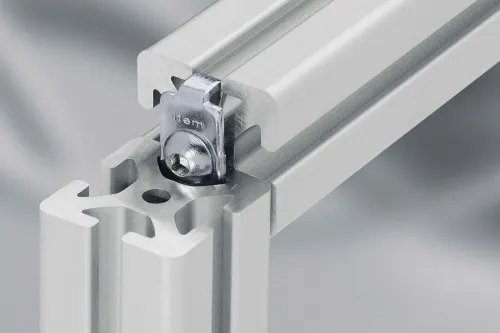
\includegraphics[width=0.3\textwidth]{Item-Standartverbindungssatz.png}
    \centering
    \caption{Item Profil mit Standartverbindungssatz, Quelle: \cite{Item_svs}}
    \label{sfs_item}
\end{wrapfigure}
\paragraph{Item}\mbox{}\\
Das Item-Profilsystem ist ein System, welches Aluminium-Extrusionen in verschiedenen Ausführungen sowie viele Verbindungsmöglichkeiten zu sich selbst sowie anderen mechanischen Elementen bietet. Hierbei gibt es eine breite Auswahl an Profilen, von 20x20 mm bis 40x40 mm Querschnitt. Für alle Komponenten mit hoher mechanischer Beanspruchung werden 40x40-Extrusionen verbaut, da diese eine besonders hohe Biegefestigkeit aufweisen. Für Anwendungen mit geringerer Beanspruchung sowie aus Platz- und Gewichtsparmaßnahmen werden 20x20-Extrusionen verwendet.
Zur Verbindung zu anderen Bauelementen gibt es die Möglichkeit, sogenannte Nutensteine mit verschiedenen Gewinden in die Nut einzulegen und dort Platten o. Ä. anzuschrauben. Um Item-Profile untereinander zu verbinden, können Standardverbindungssätze wie in Abb. \ref{sfs_item} verwendet werden.\\

Die Anwendung im AFSS erfordert ausserdem recht lange Verfahrwege. Um dies kostengünstig umsetzen zu können, werden V-Slot-Profile verwendet.


\begin{wrapfigure}{R}{0.3\textwidth}
    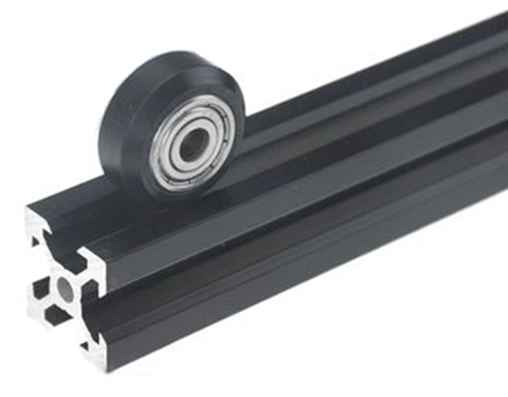
\includegraphics[width=0.3\textwidth]{V-Wheel.jpg}
    \centering
    \caption{V-Slot-Profil mit V-Wheel, Quelle: \cite{v_slot_wheel}}
    \label{v-wheel}
\end{wrapfigure}
\paragraph{V-Slot}\mbox{}\\
Auch V-Slot-Profile sind Aluminium-Extrusionen. Diese können grundsätzlich auch ähnlich wie Item-Profile mit Nutensteinen etc. verwendet werden, sind aber zusätzlich darauf ausgelegt, dass ein V-Wheel in einer Narbe des Profils rollen kann (siehe Abb. \ref{v-wheel}). Diese Profile sind in einer C-Profil-Form erhältlich. Diese sind für die langen Verfahrwege optimal, da einerseits auch breitere und mehr V-Wheels verwendet werden können, sowie einen sehr großen Widerstandsmoment aufweisen.


\subsubsection{Vorgehensweise}
Aufgrund der besonderen und sehr komplexen Anforderungen dieser Mechanik erfolgt die Entwicklung in mehreren Iterationen. Nach Auslegung der Grundparameter wird eine Grundkonstruktion erstellt, um mögliche Lösungsansätze für die jeweiligen Komponenten zu skizzieren. Durch diese grobe Planung können viele Konzepte mit geringerem Zeitaufwand iteriert werden und auch mögliche Missverständnisse o. Ä. frühzeitig aufgeklärt und überarbeitet werden. Weiters werden bei diesem Prozess wichtige Fähigkeiten in der Bedienung der CAD-Software gewonnen und so die Geschwindigkeit der zukünftigen Designiterationen beschleunigt.\\
Um bestimmte Elemente der Mechanik einzeln zu testen, werden auch mehrere Prototypen gebaut und die gewonnenen Erkenntnisse in die finale Konstruktion miteingebunden.\\

\begin{figure}[H]
    \centering
    \begin{subfigure}{.3\textwidth}
        \centering
        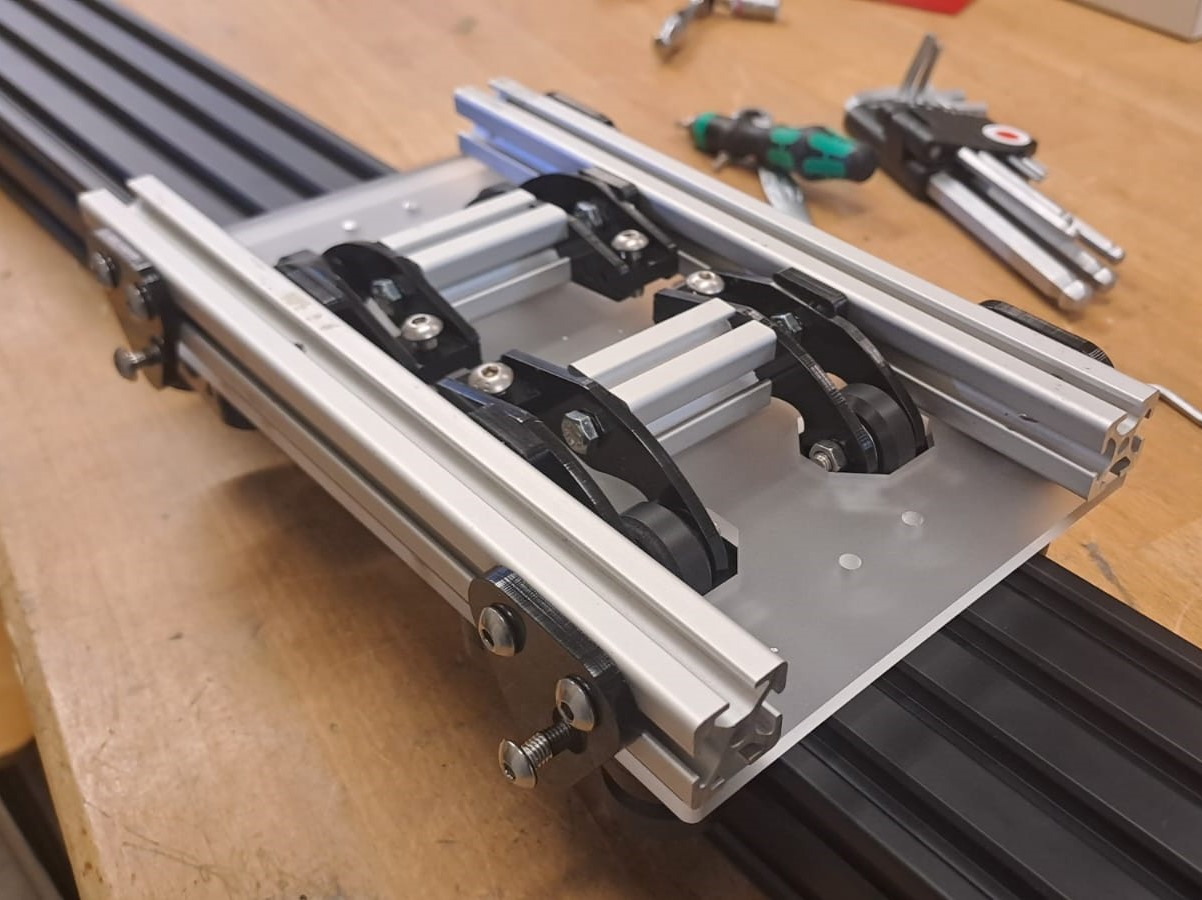
\includegraphics[width=0.9\textwidth]{pt_x.jpg}
        \caption{X-Achse}
        \label{pts:plt_x}
    \end{subfigure}%
    \begin{subfigure}{.3\textwidth}
        \centering
        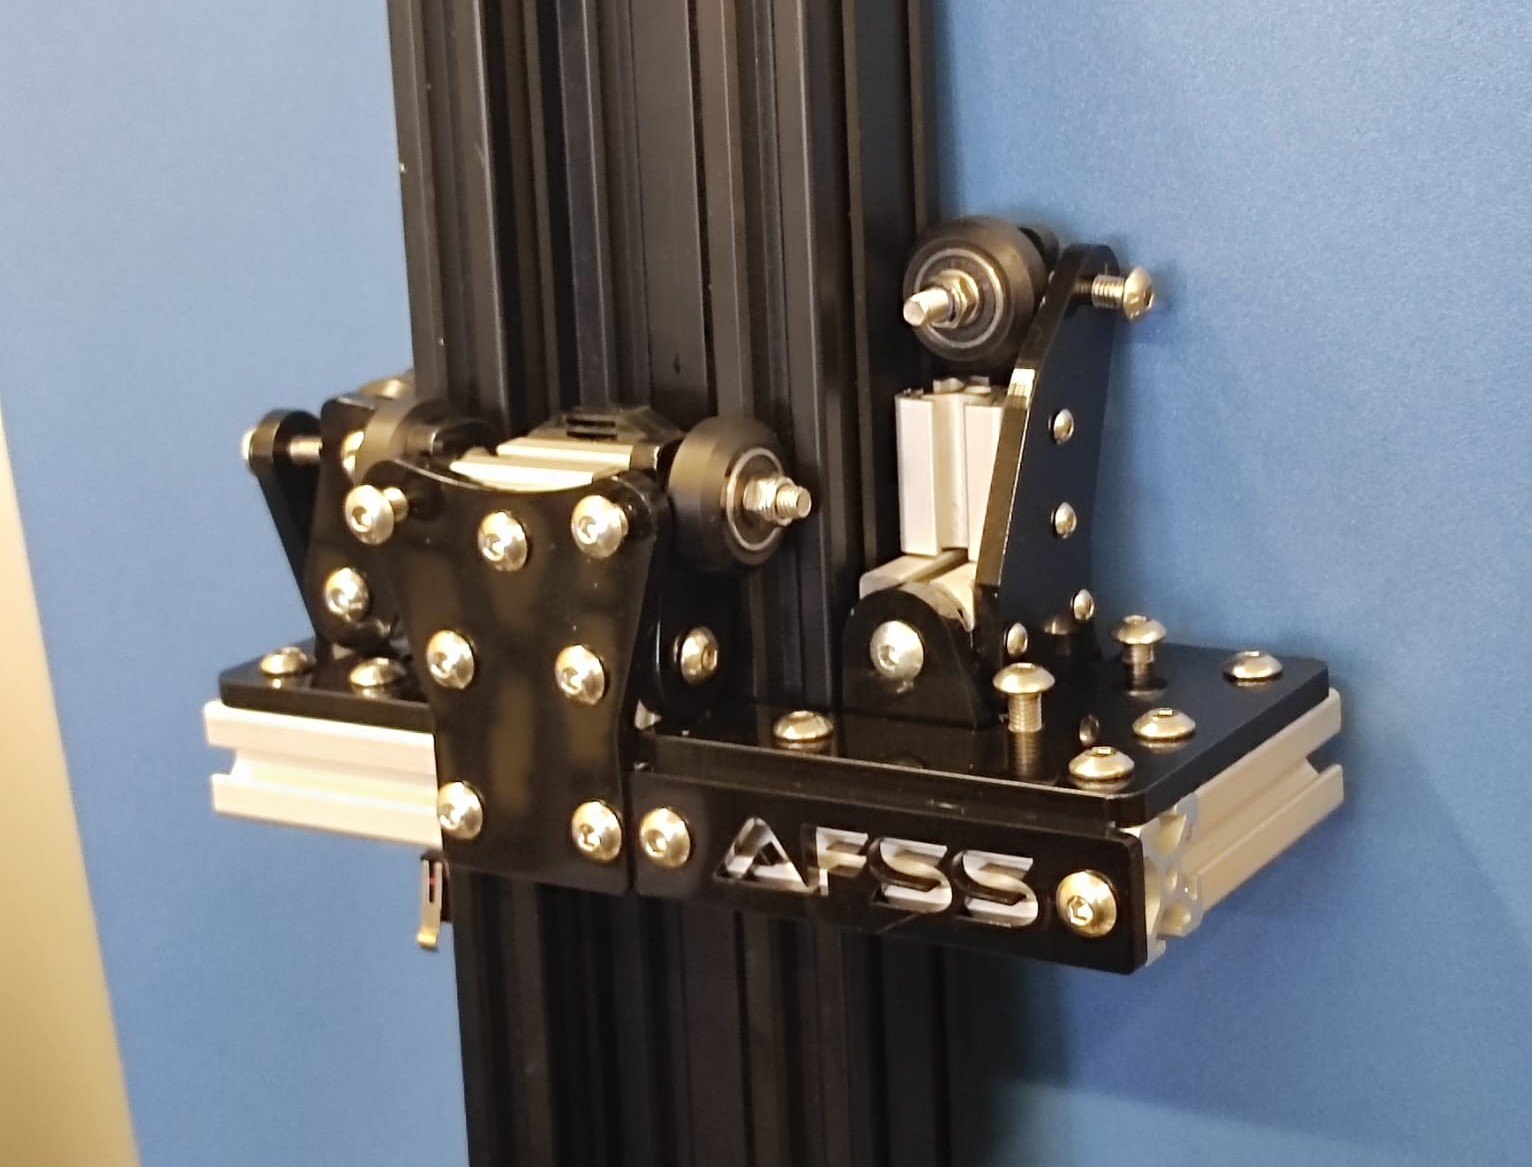
\includegraphics[width=0.9\textwidth]{pt_y.jpg}
        \caption{Y-Achse}
        \label{pts:plt_y}
    \end{subfigure}%
    \begin{subfigure}{.3\textwidth}
        \centering
        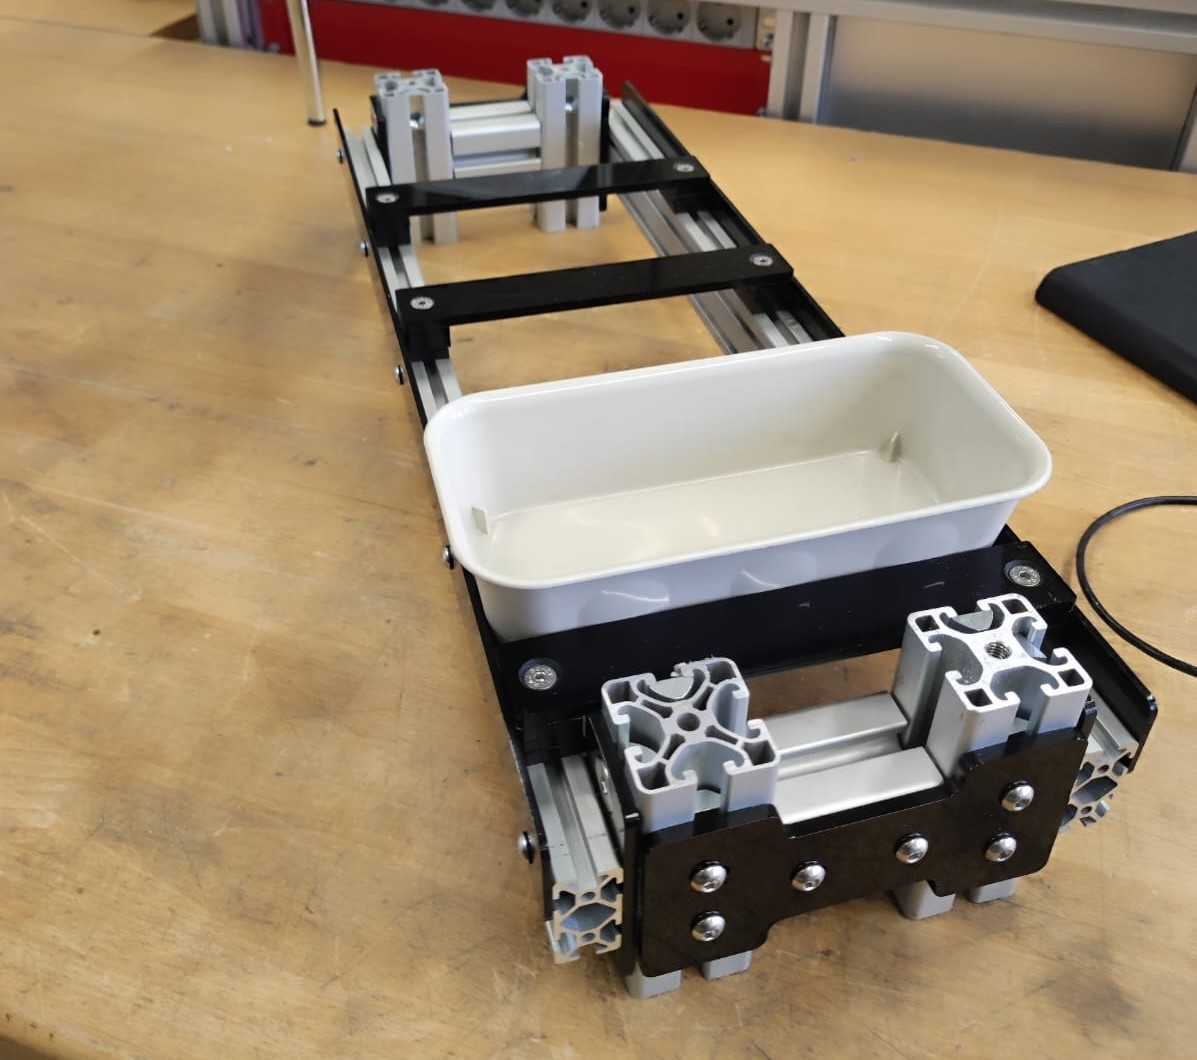
\includegraphics[width=0.9\textwidth]{pt_lg.jpg}
        \caption{Lagerregal}
        \label{pts:plt_ls}
    \end{subfigure}
    \caption{Prototypen}
    \label{pts}
\end{figure}
\vspace{-3mm}

\paragraph{Rahmenbedingungen für die Fertigung}\mbox{}\\
Damit die Fertigung der Mechanik an der HTL-Mössingerstraße in einem realistischen Zeitrahmen möglich ist, müssen gewisse Rahmenbedingungen bei der Planung beachtet werden.
\begin{itemize}
    \item Für Verbindungen mit geringer bis mittlerer mechanischer Beanspruchung werden Bauteile so geplant, dass diese im Lasercutter gefertigt werden können, sowie in den Stärken, die der Werkstätte zur Verfügung stehen (3, 4 und 5 mm). Dabei muss beachtet werden, dass die Acrylplatten gegossen sind und dadurch recht hohe Toleranzen (bis zu +0.3 mm) aufweisen.
    \item Verbindungen zwischen Platten und Item- oder V-Slot-Profilen werden möglichst einheitlich gestaltet. Grundsätzlich gilt: Verbindungen mit Item-Baureihe (BR) 5 (20x20) werden grundsätzlich in M5 ausgeführt, außer bei Platzmangel in M3. Verbindungen mit BR 8 (40x40) werden in M8 ausgeführt.
    \item Bei Bauteilen mit hoher mechanischer Beanspruchung wird Aluminiumblech mit 5 mm Stärke verwendet. Dieses wird zwar CNC-gefräst, doch um bei der Fertigung Zeit zu sparen, wird davon abgesehen, Taschen o. Ä. einzuplanen. Stattdessen wird immer ein flaches Profil verwendet, welches sich mit 2.5D-Fräsverfahren mit Durchgangsfräsen, ähnlich einem Lasercutter, fertigen lässt. Bei Aluminiumteilen wird darauf geachtet, dass diese immer aus 5 mm dickem Aluminiumeloxal gefertigt werden.
\end{itemize}

%---corrigiert----


\paragraph{Konstruktionsvorgang}\mbox{}\\
Um ein so umfangreiches Projekt umsetzen zu können, muss auch bei der 3D-Planung größtmögliche Ordnung herrschen. Um effizient zu arbeiten, werden wiederverwendbare Bauteile in einer eigens angelegten Bauteilbibliothek abgelegt. So können beispielsweise Aluminiumprofile in Normlängen oder Sensoren einfach in die aktuelle Konstruktion eingefügt werden, ohne diese jedes Mal neu konstruieren zu müssen.
\\
Auch innerhalb einer Konstruktion ist auf Übersichtlichkeit zu achten. Zu diesem Zweck ist es sinnvoll, zusammenhängende Objekte in Komponenten zusammenzufassen. Diese sind vergleichbar mit Ordnern. Wie auch Ordner können Komponenten ineinander verschachtelt werden. Dadurch lässt sich eine saubere Struktur umsetzen, die es beispielsweise erleichtert, einzelne Konstruktionsteile zu betrachten oder gezielt Änderungen daran vorzunehmen.


\subsubsection{Rahmen}

Der Rahmen des AFSS bezeichnet jene Struktur, die sowohl als äußeres Gehäuse als auch zur grundlegenden mechanischen Stabilität dient. Er soll die maximal zulässige Höhe und Länge optimal ausnutzen, während die Breite so gering wie möglich gehalten wird.
\\
Umgesetzt wird dies mit einem Gerüst aus 40x40-Aluminium-Extrusionen. Dieses besitzt zusätzlich oben und unten zwei Längsstreben, die eine möglichst platzsparende Aufhängung der X-Achsen-V-Slot-Profile ermöglichen. Auf einer Seite wird zudem eine Aussparung eingeplant, um ausreichend Freiraum zu schaffen, damit der Querförderer die Boxen reibungslos auf das Förderband transportieren kann.
\\
Weiterhin muss berücksichtigt werden, dass Rollen für den Transport angebracht werden. Da diese die maximale Höhe beeinflussen, muss dies in die Planung der Y-Achse einfließen, um sicherzustellen, dass das System problemlos durch Türen bewegt werden kann.

\subsubsection{X-Achse}
Die X-Achse des AFSS ist das mechanische Herzstück. Sie ist die Achse, die sich horizontal bewegt und einen langen Verfahrweg sowie hohe mechanische Anforderungen besitzt. Sie muss sowohl ihr Eigengewicht als auch das Gewicht der YZ-Achse tragen.
\\
Das Grundelement der X-Achse besteht aus V-Slot-C-Profilen, die oben und unten aufgehängt werden. Diese Profile sind in Längen von 1,5 m erhältlich, daher wird die gesamte Achse so ausgelegt, dass zwei Stück (also insgesamt 3 m Schiene) verwendet werden. Zusätzlich sind die Profile mit jeweils sechs Nivellierungsschrauben pro V-Profil ausgestattet, um sie möglichst parallel zueinander sowie exakt in Waage auszurichten.

\paragraph{Grundanforderungen}\mbox{}\\
Auf der X-Achse bewegt sich der X-Schlitten, dessen Aufgabe es ist, die Y-Achse präzise zu positionieren. Dafür muss er alle erforderlichen Motoren und Sensoren enthalten. Zudem muss er einen Angriffspunkt bieten, um seine Bewegung zu ermöglichen.
\\
Der Schlitten sollte sowohl horizontal als auch vertikal möglichst kompakt konstruiert sein, um einen maximalen Verfahrweg in X- und Y-Richtung zu gewährleisten.

\paragraph{Antrieb}\mbox{}\\
Angetrieben wird die X-Achse mit zwei Schrittmotoren, welche jeweils an einer Schiene (oben und unten) angebracht werden. Diese treiben mithilfe eines Zahnriemens die zwei X-Schlitten an. Als Zahnriemen wurde aufgrund der hohen Kraftübertragung sowie der großen Länge ein AT5-Zahnprofil mit 16 mm Riemenbreite der Firma Mähdler gewählt. Dieser wird vom Motor über eine entsprechende Zahnscheibe angetrieben und am Shuttle befestigt. Als Schrittmotor wird aus Einfachheitsgründen dasselbe Modell wie bei der Y-Achse verwendet. Diese erzeugen auch genügend Moment, um die X-Achse anzutreiben.

\paragraph{Riemenspannung X-Achse} \mbox{}\\
Da der Riemen für eine zuverlässige Kraftübertragung bei so langen Verfahrwegen eine relativ große Vorspannkraft benötigt, ist das Zahnriemenklemmelement auf der X-Achse auch dementsprechend auszuführen. Um den Zahnriemen zu greifen, muss ein Negativ in Aluminium gefräst werden, in dieses der Zahnriemen dann auf beiden Seiten des Schlittens geklemmt wird. Die Aufhängung der einen Seite ist einfach mit den Item-Profilen verschraubt, lässt aber noch etwas Platz, um den Riemen mit der Hand vorzuspannen. Auf der anderen Seite ist das Klembrett über zwei Gewindestangen mit dem restlichen Shuttle verbunden. Diese können festgezogen werden, um die nötigen Vorspannkräfte zu erzeugen. Außerdem ist diese Spannvorrichtung in einem Formfaktor ausgeführt, welcher es erlaubt, direkt darüber die Motoren der Y-Achse anzubringen.

\paragraph{Achsenführung} \mbox{}\\
Die Führung der Achse im V-Slot-Profil wird mit V-Wheels durchgeführt. Sechs V-Wheels werden von oben auf das C-Profil gedrückt. Jedes Rad wird einzeln aufgehängt. Weiters ist überall eine Schraube, mit welcher das Rad weiter in die Führung hineingedrückt werden kann, sowie ein bis zwei Klemmpunkte, um bei Betrieb die Last von der Spannschraube nehmen zu können. Durch den geringen Platz im Schlitten ist es durchaus eine Herausforderung, dass all diese Mechanik neben den Spannelementen und Motoren in einem so kleinen Shuttle Platz finden. Auf der Seite des Schlittens werden noch weitere V-Wheels angebracht, welche die Spurführung übernehmen.
Im oberen Schlitten werden nur diese Führungsräder verbaut, da es nicht möglich und nötig ist, vertikale Kräfte zu unterstützen.

\paragraph{Kabelführung} \mbox{}\\
Um Sensoren und Aktoren der Y- und Z-Achse zu unterstützen, müssen dementsprechende Leitungen auf das X-Shuttle verlegt werden. Dies wird mithilfe einer Kabelschleppkette der Firma Igus umgesetzt. Diese wird parallel zum unteren C-Profil verlegt und unter Berücksichtigung der Biegeradien am X-Shuttle befestigt. Bei dieser ist darauf zu achten, dass sie alle benötigten Leitungen sowie genügend Freiraum für die Biegung einhält \cite{igus_freitragend}. Weiters müssen Signal- und Aktorstromkreise durch Trennstege voneinander getrennt werden.
\\
Um die weiteren Geräte am AFSS zu versorgen, müssen zusätzlich noch Verdrahtungskanäle am Rahmen angebracht werden.

\paragraph{Sensoren}\mbox{}\\
Die Sensorik ist bei jeder Achse ähnlich aufgebaut. Immer zwei Endschalter und ein Referenzierschalter. Bei der X-Achse werden als Endschalter mechanische Rolltaster verwendet. Diese werden neben den V-Slot-Profilen befestigt und von einem, vom Schlitten abstreifenden Arm ausgelöst.

\subsubsection{Y-Achse}
Als Y-Achse wird jene Achse bezeichnet, die ihre Bewegung vertikal durchführt. Sie hat die Aufgabe, die Z-Achse bzw. das YZ-Shuttle auf Position zu bringen. Wichtig hierbei ist jedoch, dass die Y-Achse die Aufgabe des Aufhebens der Box übernimmt.

\paragraph{Antriebsauslegung}\mbox{}\\
Dadurch, dass die Y-Achse sowohl das YZ-Shuttle als auch die Boxen aufheben muss, muss der Antrieb dementsprechend dimensioniert werden. Als Formfaktor soll ein Nema23-Schrittmotor verwendet werden. Diese sind weit verbreitet und im Vergleich zu Servomotoren relativ kostengünstig. Als Grundformfaktor wird ein 2 Nm Motor gewählt. Nun soll überprüft werden, ob dieser die Last der YZ-Achse auch antreiben kann.

\vspace{5mm}
\noindent\begin{minipage}{\textwidth}
\begin{minipage}[t]{0.5\textwidth}
    \begin{equation*}
        F = \frac{M}{\frac{d}{2} \cdot 1000} \cdot n
    \end{equation*}
    \begin{equation*}
        F = \frac{2 \unit{Nm}}{\frac{30 \unit{mm}}{2} \cdot 1000} \cdot 2 = 266 \unit{N}
    \end{equation*}
\end{minipage}%
\begin{minipage}[t]{0.4\textwidth}
    \vspace*{-5mm}
    \begin{align*}
        &F: \text{Antriebskraft der Y-Achse} & &\left[N\right]\\
        &M: \text{Drehmoment eines Motors} & &\left[Nm\right]\\
        &d: \text{Durchmesser der Antriebszahnscheibe} & &\left[mm\right]\\
        &n: \text{Anzahl der Antriebe} & &
    \end{align*}
\end{minipage}
\end{minipage}

\vspace{5mm}

Bei der Konstruktion einer früheren Version des YZ-Shuttles wurde erfasst, dass das Shuttle bis zu 13 kg wiegen kann. Dies wird zwar in einer späteren Iteration des Designprozesses noch verbessert, dient jedoch als Richtwert für die Antriebsauslegung. 13 kg erzeugen ohne Berücksichtigung von Reibung knapp 130 N. Die Antriebskraft der Schrittmotoren reicht auf jeden Fall aus. Doch diese Überdimensionierung ist unter dem Aspekt, dass die Antriebe über keine Bremse verfügen und somit das gesamte Gewicht der Z-Achse sowie der Kabelschleppkette immer unterstützt werden müssen, durchaus sinnvoll.

\paragraph{Zahnriemen und Umlenkung}\mbox{}\\
Als Zahnriemen wird auch bei der Y-Achse auf ein AT5x16-Profil gesetzt. Doch hier gestaltet sich die Positionierung ebendieses nicht so simpel wie bei der X-Achse. Da der Zahnriemen beim YZ-Shuttle an einem bestimmten Punkt befestigt werden muss, muss er auch dort wieder rückgeführt werden. Die Umlenkung des Zahnriemens gestaltet sich jedoch wesentlich anspruchsvoller als bei der X-Achse, da einerseits ein möglichst kompakter Formfaktor angestrebt werden muss und andererseits eine aufhängungstechnisch sehr unvorteilhafte Positionierung vor dem V-Slot-C-Profil erforderlich ist. Aus diesem Grund wird eine Konstruktion aus Aluminium, welche sich selbst verhakt, konstruiert. Sie muss seitlich an den Profilen verschraubt werden. Im vorderen Überhang werden Aluminiumelemente eingehängt, die die Aufhängung der Achse für die Umlenkung erlauben.

\paragraph{Zahnriemenaufgängung}\mbox{}\\
Um die optimale Position der Zahnriemenaufhängung für die Y-Achse bestimmen zu können, wird überschlagsmäßig ein Massenschwerpunkt in Z-Richtung berechnet. Um mit der Konstruktion beginnen zu können, werden hierfür ungefähre Werte angenommen.

\noindent\begin{minipage}{\textwidth}
\begin{minipage}[t]{0.5\textwidth}
    \vspace{7mm}
    \begin{equation*}
        X_s = \frac{1}{M} \cdot \displaystyle\sum_{i = 0}^{n} z_i \cdot m_i
    \end{equation*}
\end{minipage}%
\begin{minipage}[t]{0.5\textwidth}
    \begin{align*}
        &Z_s: \text{Z-Koordinate des Massenschwerpunkts} & &\left[m\right]\\
        &M: \text{Gesamtmasse} & &\left[kg\right]\\
        &z_1: \text{Z-Koordinate der Teilmasse} & &\left[m\right] \\
        &m_1: \text{Masse der Teilmasse} & &\left[kg\right]
    \end{align*}
\end{minipage}
\end{minipage}

\begin{table}[H]
    \centering
    \centering
        \begin{tabular}{c c c}
            Gegenstand & Masse in kg & Position in mm\\
            \hline
            Motor & 0.3 & 21 \\
            Z-Schiene & 1 & 150 \\
            Z-Gable & 0.3 & 180 
        \end{tabular}
    \caption{X-Achse unbeladen und eingefahren}
        \vspace{5mm}
        \centering
        \begin{tabular}{c c c}
            Gegenstand & Masse in kg & Position in mm\\ 
            \hline
            Motor & 0.3 & 21 \\
            Z-Schiene & 1 & 150 \\
            Z-Gabel & 1.3 & 380
        \end{tabular}
        \caption{X-Achse beim Ladevorgang}
\end{table}
So werden zwei Schwerpunkte errechnet: ca. 130 mm im unbeladenen Zustand und 250 mm während dem Ladevorgang. Da die Stabilität des Y-Shuttles während dem Ladevorgang wichtiger ist als während einer Leerfahrt, wird das Y-Shuttle so positioniert, dass die Aufhängung des Zahnriemens bei rund 200 mm liegt.\\
Weiters muss auch dieser Zahnriemen wieder gespannt werden. Durch die geringere Zahnriemenlänge wird auch der Spannmechanismus verkleinert.
Leider muss dieser aus Platzgründen außerhalb der Flucht zum Zahnriemen angebracht werden. Die Folgen dieser Auslenkung auf die Riemenspannung können durch folgenden Ausdruck, der die Länge, die der Zahnriemen bei einer bestimmten Position braucht, um spannungslos zu sein, approximiert, ermittelt werden. (Hierbei wird von einem linearen Zusammenhang zwischen der Kraft auf die Aufhängung und der Längenkontraktion ausgegangen. In der Realität würde jedoch die Elastizität des Zahnriemens sowie jene der Aufhängung Auswirkungen haben, aber diese verringern die Auswirkungen nur zu unseren Gunsten).
    \vspace{4mm}
    \noindent\begin{minipage}{\textwidth}
    \begin{minipage}[t]{0.5\textwidth}
        \begin{equation*}
            K(h) = \sqrt{h^2+d^2}+(l-h)
        \end{equation*}
        \begin{equation*}
            K(h) = \sqrt{h^2+28^2}+(1500-h)
        \end{equation*}
    \end{minipage}%
    \begin{minipage}[t]{0.5\textwidth}
        \vspace{-7mm}
        \begin{align*}
            &K(h): \text{theoretische Länge des Riemen} & &\left[mm\right]\\
            &h: \text{Position des Schlittens} & &\left[mm\right]\\
            &l: \text{Umlenkungsrollenabstand} & &\left[mm\right]\\
            &d: \text{Abstand der Klemme zur Flucht} & &\left[mm\right]
        \end{align*}
    \end{minipage}
    \end{minipage}

    \begin{figure}[H]
        \centering
        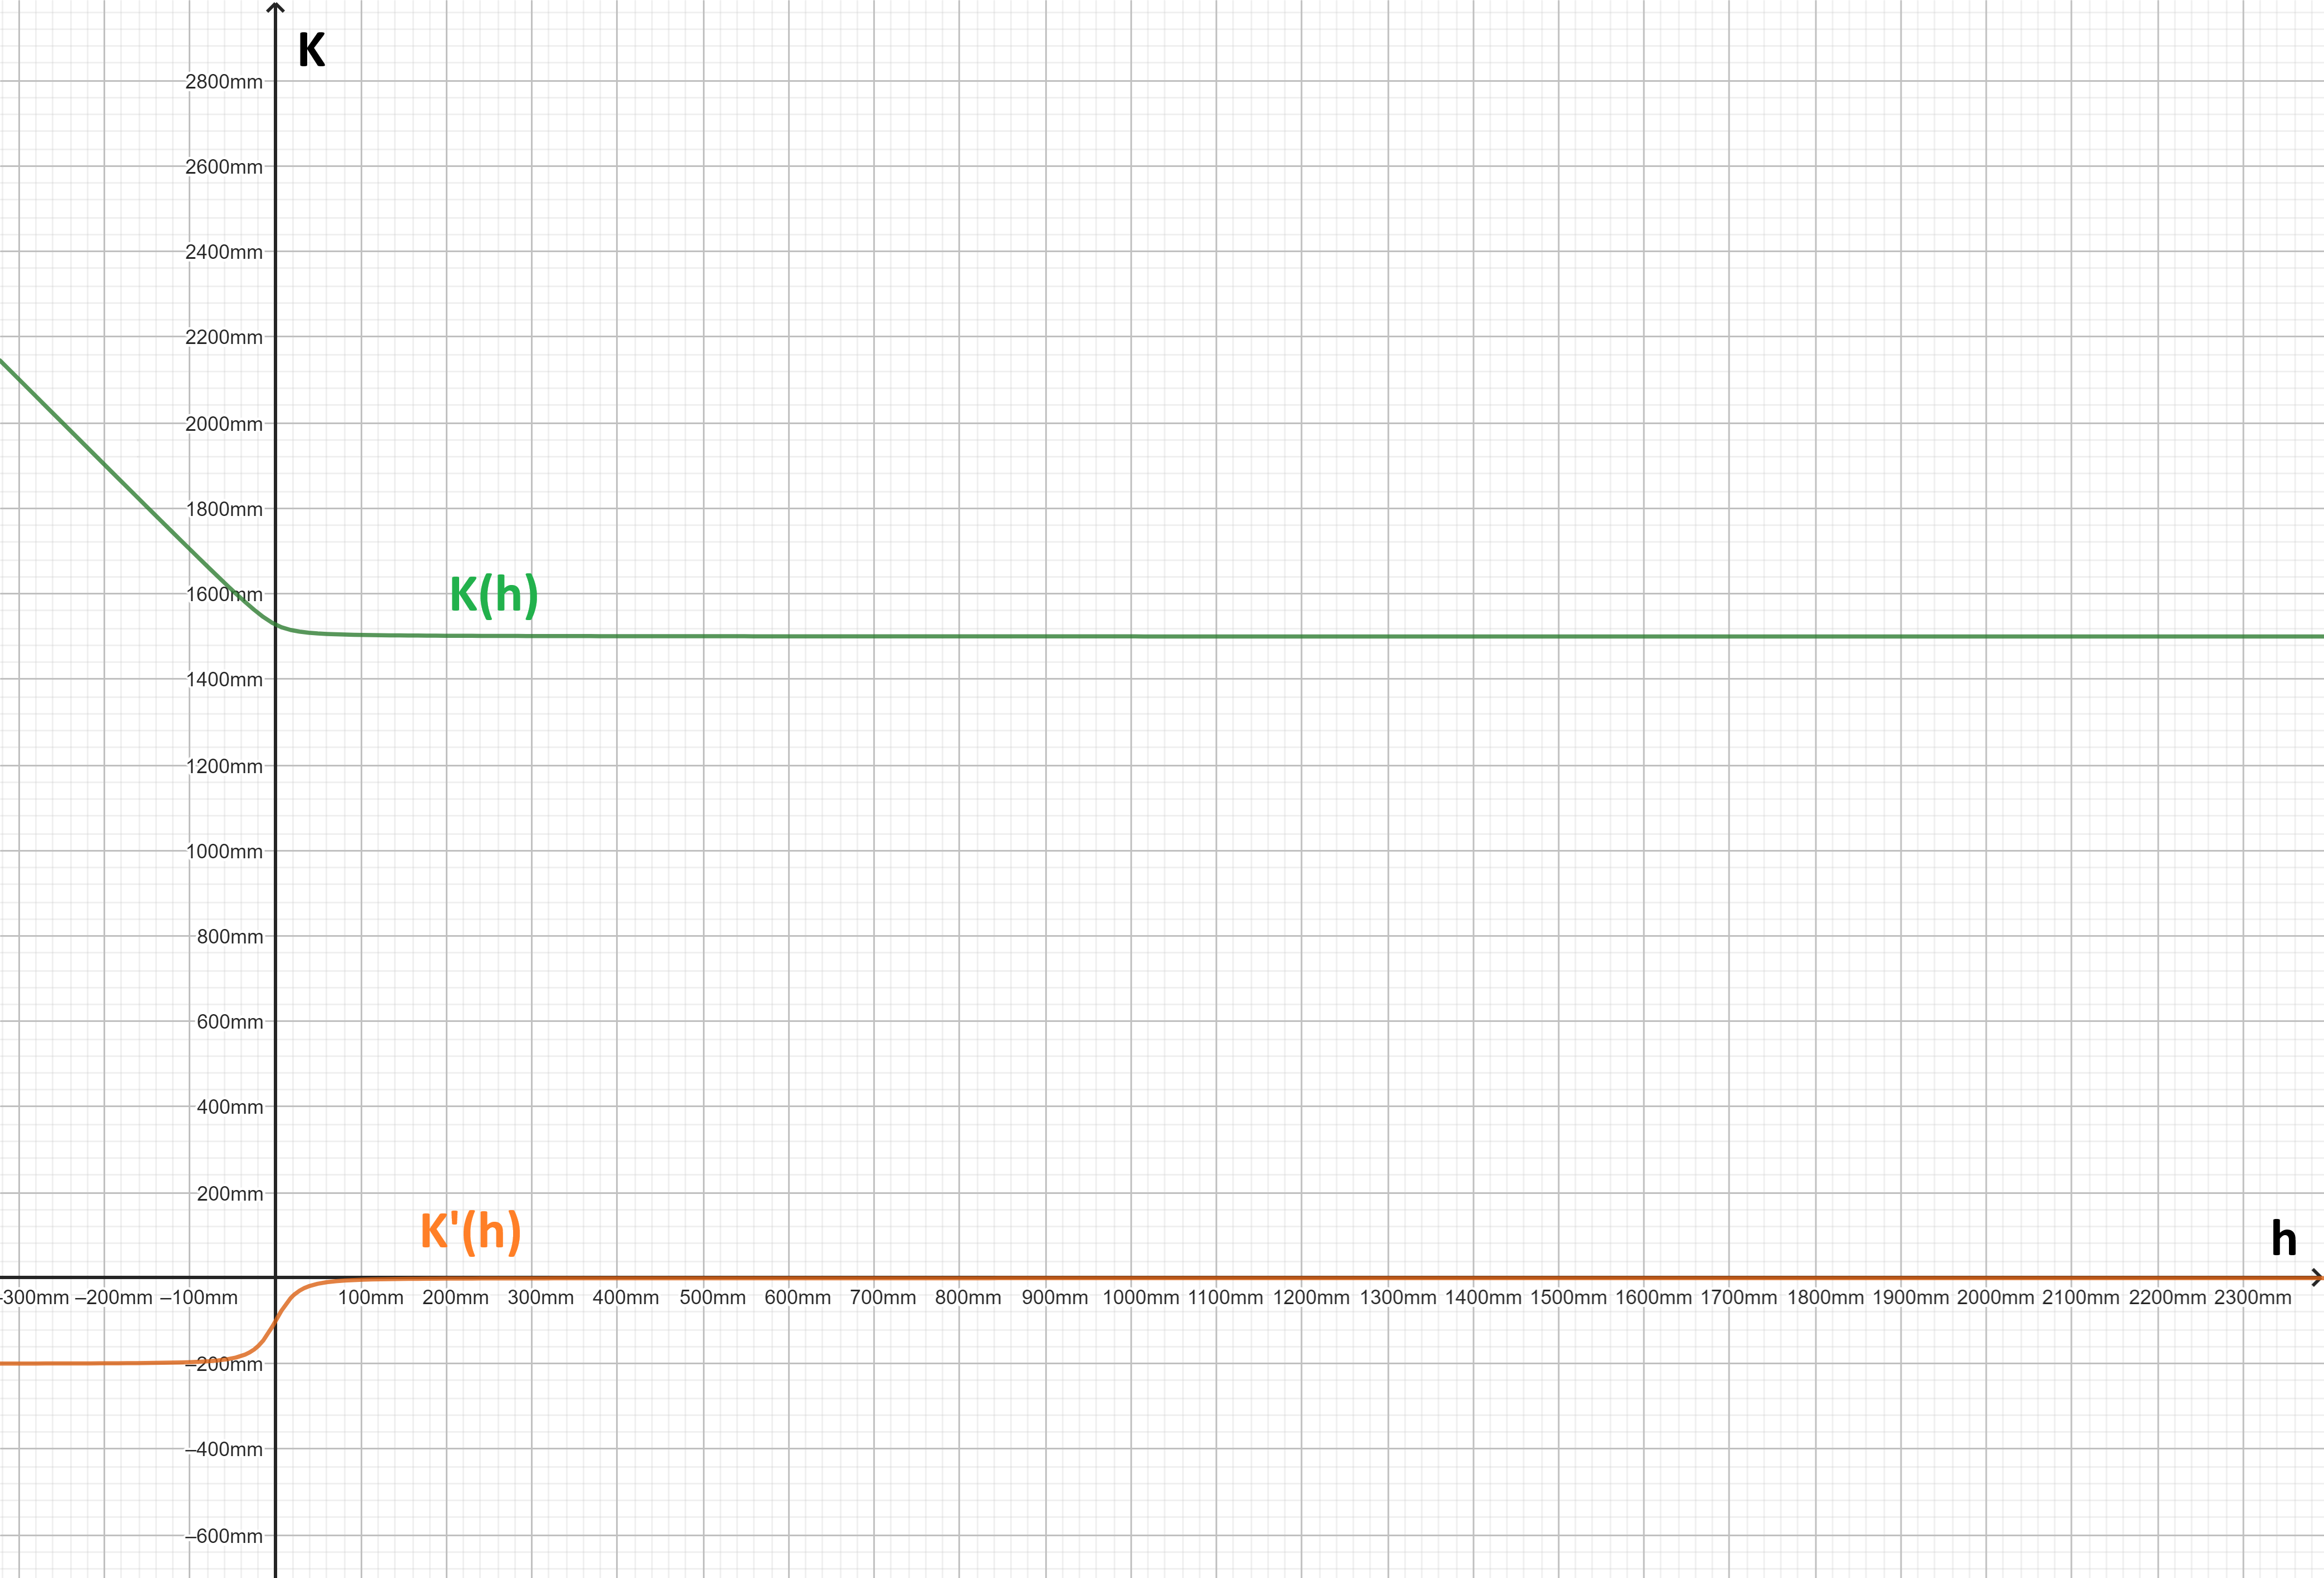
\includegraphics[width=0.7\textwidth]{Zahnrimenenversatz.png}
        \caption{Zahnriemenkontraktion grafisch dargestellt}
        \label{zahnriemenversatz}
    \end{figure}

    Aus der Abbildung \ref{zahnriemenversatz} geht, wie schon intuitiv vermutet, hervor, dass diese Asymmetrie nur dann ein Problem darstellt, wenn der Schlitten weit unten ist. Ein konkretes Maß kann folgendermaßen ermittelt werden: \(K(80) - (750) = 4.24 \unit{mm}\). Der Unterschied in der benötigten Riemenlänge zwischen der Mittelstellung (750 mm) und der Ruheposition (80 mm über der Zahnscheibe) beträgt also rund 4 mm. Im Hinblick darauf, dass diese Länge auf zwei Seiten (Hin- und Rücklaufseite) des Zahnriemens aufgeteilt wird (welcher etwas elastisch ist), sowie dass eine leichte Biegung in der Umlenkungsaufhängung auftritt, wird diese Extraspannung toleriert.

\paragraph{Shuttleführung}\mbox{}\\
Das YZ-Shuttle wird aus Stabilitätsgründen ebenfalls mit einem V-Slot C-Profil geführt. Diese sind auf beiden Seiten jeweils oben und unten befestigt. Die Länge wird so gewählt, dass die Verwendung eines 1.5 m langen Profils perfekt ausreicht. Da das YZ-Shuttle wesentlich weniger Kraft auf die Führung auswirkt, können weniger Führungsräder verwendet werden. Die Hauptführungsräder werden so positioniert, dass sich ein Dreieck ergibt. Dieses dient dazu, dass sowohl beim Aufhebevorgang als auch beim Leerlauf immer eine Klemmung um die Führungsschiene entsteht. Hierbei sind jene V-Wheels, welche beim Aufhebevorgang belastet werden, doppelt ausgeführt. Wie schon bei der X-Achse sind auch hier wieder alle V-Wheel-Abstände mit Schrauben einstellbar. Zusätzlich zur Hauptführung sind auch außen jeweils noch zwei Führungsräder angebracht, um das Shuttle zusätzlich zu stabilisieren.

\paragraph{Sensoren}\mbox{}\\
Da die Endschalter der Y-Achse kapazitiv ausgeführt sind, muss auf dem Shuttle ein metallisches Gegenstück angebracht sein. Diese stehen oben und unten über und lösen so vor Kollision aus. Um die Sensoren anzubinden, muss auch ein ASi-Client auf dem X-Shuttle angebracht werden.

\paragraph{Kabelschleppkette}\mbox{}\\
Um Versorgung der Z-Achse herstellen zu können, muss eine Kabelschleppkette vom X- zum Y-Shuttle angebracht werden. Ach diese muss leider Sonderanforderungen erfüllen. Da die Versorgung von unten ausgeht, muss die Kabelschleppkette stehend eingebaut werden. Dies ist grundsätzlich eine äußerst ungünstige Situation, da diese Schleppkette der Beschleunigung des X-Shuttles ausgesetzt ist. Um ein Schwingen möglichst zu verhindern, werden seitlich noch Führungselemente angebracht. Außerdem sind die Anschlusselemente fest um die ersten Kettenglieder extra zu unterstützen. \cite{igus_vertikal}

\subsubsection{Z-Achse}
Als Z-Achse oder Gabel, wird jener Teil des AFSS bezeichnet, der die Boxen in das Lager ein- und ausfährt. Dieser ist in das YZ-Shuttel integriert. Es wird davon ausgegangen, dass um Boxen ein- und auszuheben ca. 210 mm überstand der Gabel benötigt wird. Dies ist also der Mindestverfahrweg der Z-Achse

\paragraph{Linearführung}\mbox{}\\
Geführt wird die Gabel mit zwei Führungsschienen von Igus. Diese bieten optimale Stabilität sowie, in Verbindung mit einem Führungswagen, eine reibungsarme Bewegung. Wichtig ist jedoch, dass der Schwerpunkt der am Führungswagen befestigten Last nicht mehr als die doppelte Wagenlänge über den Wagen hinausgeht. Danach kommt es zu sehr starker Verklemmung, und ein Betrieb ist nur mehr schwer möglich. Da bei einer Auslegeroperation der Schwerpunkt sehr weit übersteht, wird eine TS-01 Führungsschienen- und -wagenkombination verwendet. Diese wirkt zwar recht überdimensioniert, doch da der Führungswagen so lang ist, kann ein reibungsarmer Betrieb gewährleistet werden.

\paragraph{Motor}\mbox{}\\
Als Antrieb für die Z-Achse sollen zwei Nema-17 Schrittmotoren verwendet werden. Hier ist es nicht nötig, eine Closed-Loop-Steuerung zu verwenden, da bei jedem Hub auch referenziert werden kann. Weiterhin kann dadurch Kabelschleppkettenplatz gespart werden.

\paragraph{Spindelauslegung}\mbox{}\\
Die Z-Achse wird mit einer Spindel angetrieben. Dies bietet Vorteile in der Positionsgenauigkeit und der Kraftübertragung. Jedoch ist es wichtig, die richtige Spindelsteigung auszuwählen, um die Balance zwischen Geschwindigkeit und Kraft zu halten. Ziel ist es, für eine Richtung des Hubs maximal 5 Sekunden zu benötigen. Sie wird über eine Zahnscheibe und Zahnriemen mit dem Motor verbunden.\\
Berechnet werden kann diese Zeit mit folgendem Ausdruck:

\vspace{5mm}
\noindent\begin{minipage}{\textwidth}
\begin{minipage}[t]{0.5\textwidth}
    \vspace{10mm}
    \begin{equation*}
        v = \frac{k}{n_{welle}} = \frac{k}{\frac{n_{motor}}{i}}
    \end{equation*}
    \begin{equation*}
        F = \frac{M_{mot} \cdot i \cdot k}{n_{welle}} \cdot 2 \pi f \cdot \eta 
    \end{equation*}
\end{minipage}%
\begin{minipage}[t]{0.5\textwidth}
    \vspace{-7mm}
    \begin{align*}
        &M_{mot}: \text{Drehmoment} & &\left[\frac{N}{m}\right]\\
        &n_{mot}: \text{Drehzahl} & &\left[\frac{1}{s}\right]\\
        &k: \text{Wellensteigung} & &\left[\frac{mm}{U}\right]\\
        &i: \text{Übersetzungsverhältniss} & \\
        &\eta: \text{Wirkungsgrad der Gewindeshraube} & \\
    \end{align*}
\end{minipage}
\end{minipage}

\vspace{5mm}

So wird berechnet, dass eine DS10x12-Spindel mit ihrer 12 mm Steigung, bei einer Motordrehzahl von 600 U/min (0.42 Nm) und einem Übersetzungsverhältnis von 2:1, ca. 4 Sekunden pro Richtung benötigt und mit einer Kraft von ca. 90 N bewegt wird.\\
Dies entspricht unseren Anforderungen, und somit wird diese Spindel gewählt. Um sie zu lagern, wird vorne und hinten der Durchmesser der Spindel verringert, sodass diese in Kugellagern geführt werden kann.

\paragraph{Sensorik}\mbox{}\\
Um auch die Endschalter der Z-Achse, sowie weitere Sensoren einzulesen, wird auch hier ein ASi-Slave montiert.

\subsubsection{Lager}
Das Lager soll die Boxen beinhalten und die Möglichkeit zulassen, dass diese von der Gabel ein- und ausgehoben werden. Weiterhin muss die Box in X- und Z-Richtung geführt werden, um die Positionsgenauigkeit sicherzustellen, da sonst die Gabel möglicherweise in die Box fährt. Das Lager soll darauf ausgelegt werden, dass Boxen mit den Maßen 50x100x200 mm verwendet werden können. Diese Boxen sind nach unten hin verjüngt und haben oben eine Lippe, an der die Gabel greift.
Umgesetzt wird dies mit einem Gerüst aus 40x40-Item-Profilen, welches im Nachhinein in den restlichen Rahmen eingesetzt wird. Auf diese werden 20x40-Profile horizontal aufgeschraubt, auf denen die Boxen stehen. Vorne und hinten wird eine Kunststoffplatte aufgeschraubt, welche leicht übersteht und somit die Box in Z-Richtung positioniert. Zwischen den Boxen wird ein Trennsteg eingebaut, welcher die Boxen in X-Richtung positioniert sowie den richtigen Abstand zwischen den Boxen einhält.

\subsubsection{Querförderer}
Da es dem Portalroboter nicht möglich ist, die Boxen direkt auf das Förderband zu legen, muss hier noch ein System eingebaut werden, welches dies erledigt. Da die Boxen beim Ein- und Auslagern den gleichen Weg zurücklegen, muss dieser Querförderer die Box sowohl auf das Förderband als auch vom Förderband herunterbewegen können.\\
Zu diesem Zweck wird eine weitere, der Gabel ähnliche Konstruktion montiert, welche auf einem 20x40-V-Slot-Profil verläuft. Die Box wird dann hin- und hergeschoben, um vom Lager auf das Förderband umzuladen. Dadurch ist es noch möglich, dass die Gabel der Z-Achse die Box in der Nullstellung ein- und aushebt.


\subsubsection{Fertigung der Einzelteile}

\paragraph{Umlenkrollen}\mbox{}\\
Die Umlenkrollen sind jeweils am Ende der X- und Y-Achsen angebracht. Da diese der gesamten Spannkraft ausgesetzt sind, erfordert dies spezielle Anforderungen an die Aufhängung sowie an die Umlenkrolle selbst. Diese soll primär eine 180°-Wende des Zahnriemens ermöglichen und sekundär eine Führung für den Riemen bieten.\\
Um diese Anforderungen umzusetzen, werden vier Aluminium-Drehteile gefertigt, in welche Kugellager eingepresst werden.

\begin{figure}[H]
    \centering
    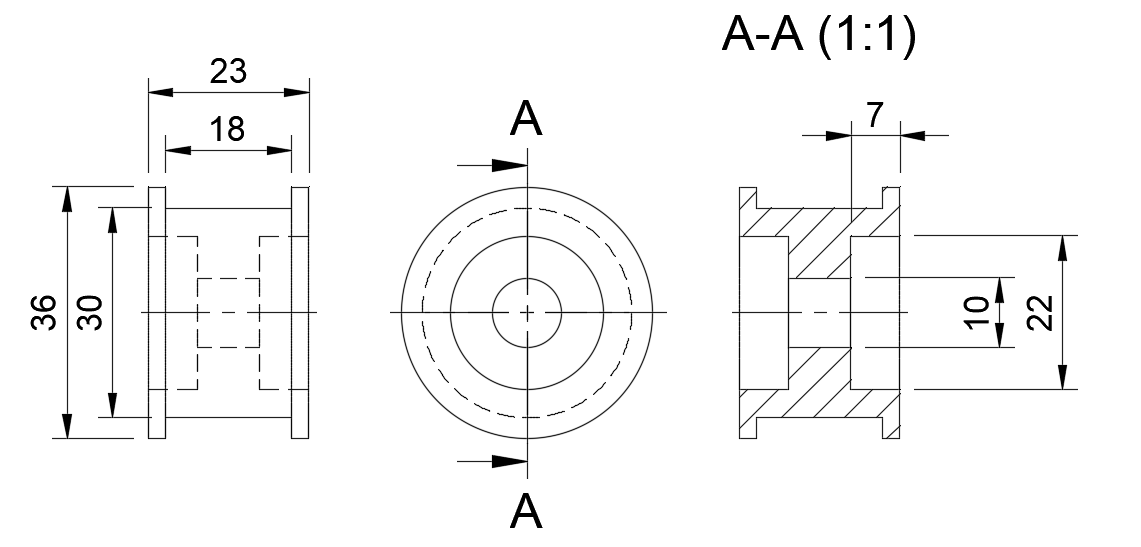
\includegraphics[width=0.8\textwidth]{AT5x16-Umlenkung.png}
    \caption{Bauteilzeichnung Umlenkrolle}
    \label{UmlenkrolleBTZ}
\end{figure}

Die Fertigung dieses Teils nach Abb. \ref{UmlenkrolleBTZ} lässt sich in folgende Teilschritte unterteilen:
\begin{itemize}
    \setlength\itemsep{-1mm} 
    \item Zuerst die Frontfläche plandrehen (Drehzahl: 900 U/min)
    \item Ungefähr 30mm Länge auf das Aussenmaß von 36 mm längsdrehen
    \item Mit 9.8mm Bohrer das mittlere Loch vorbohren (540 U/min)
    \item Mit 10mm Reibeisen und viel Öl das Loch auf eine genaue Passung bringen (260 U/min)
    \item Die Position relativ zum Backenfutter markieren, um beim Neu-Einspannen Rundlaufgenauigkeit zu gewährleisten
    \item Zylinder bei ca. 26 mm abstechen (540 U/min)
    \item Umspannen und auf Maß plandrehen (900 U/min)
    \item Die Aussparung für die Lager mit Eckdrehmeißel beginnen, jedoch nach innen hin nur 6.8 mm
    \item Bei ca. 17 mm Lochdurchmesser den tatsächlichen Durchmesser mit der Digitalanzeige vergleichen und gegebenenfalls korrigieren
    \item Bei 21.5 mm den Oberschlitten die restlichen 0.2 mm zustellen und die gesamte Tiefe plandrehen
    \item Den Lochdurchmesser auf 21.95 erweitern und dann in kleinen Inkrementen zustellen, bis das Lager gerade so nicht passt, um einen Presssitz zu gewährleisten. Dies tritt bei Lagern mit 22 mm Außendurchmesser bei rund 22.04 mm ein.
    \item Da für die Einsparung der Riemenführungsfläche kein Angriffspunkt verfügbar ist, wurde als Halterung ein Dorn nach Abb. \ref{ulr:dorn} gedreht, auf welchen das Drehteil aufgeschraubt wird.
    \item Mit dem Abstechmeißel wird in 2 mm Inkrementen die Zahnriemenauflagefläche herausgedreht, bis auf 30.2 mm, sowie links und rechts den Rand 1 mm extra dick lassen (siehe Abb. \ref{ulr:f1} ). (540 U/min)
    \item Am Schluss wird die Rand Tiefe auf Maß gedreht.
    \item Als letzten Schritt werden links und rechts die zwei Lager eingepresst.
\end{itemize}

    Durch die verhältnismäßig großen Toleranzen bei den Lageraussendurchmessern wird bei 2 der 8 Lagerpassungen zusätzlich Lagerkleber verwendet, um einen zuverlässigen Halt zu gewährleisten, da bei diesen die Toleranzen nicht eingehalten wurden.\\
    Nach diesem Vorgang sind die vier Umlenkrollen fertig (siehe \ref{ulr:f2}) und können auf einem 8-mm-Schaft montiert werden.

    \begin{figure}[H]
        \centering
        \begin{subfigure}{.3\textwidth}
            \centering
            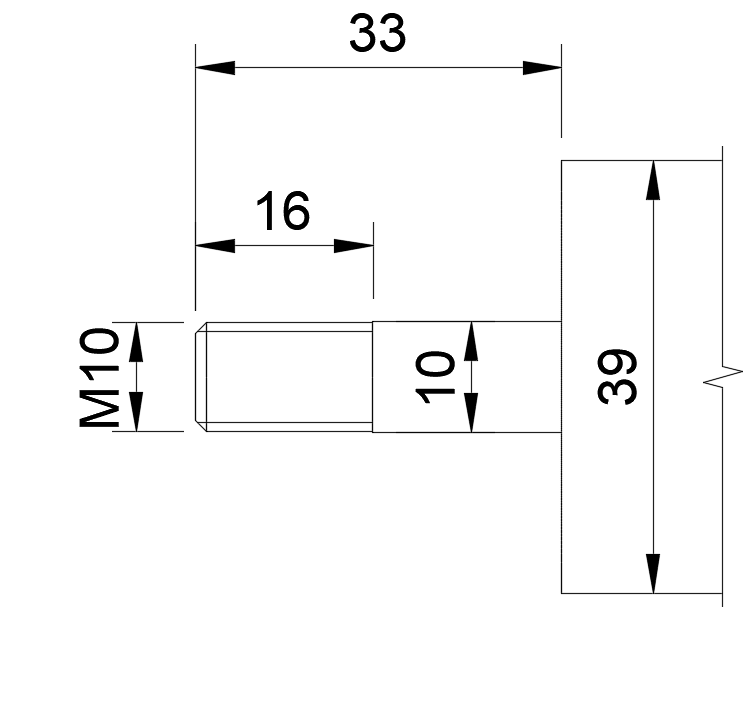
\includegraphics[width=0.9\textwidth]{AT5x16-Umlenkung-Dorn.png}
            \caption{Dorn}
            \label{ulr:dorn}
        \end{subfigure}%
        \begin{subfigure}{.3\textwidth}
            \centering
            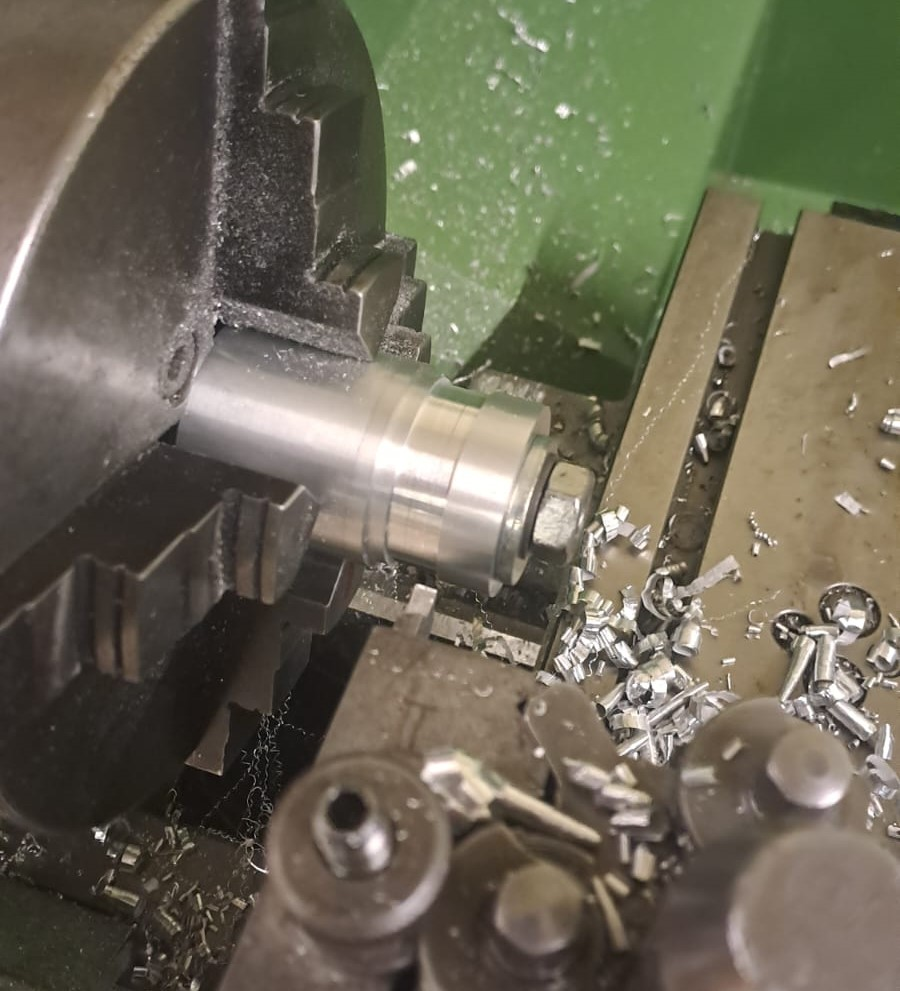
\includegraphics[width=0.9\textwidth]{ulr-fertigung.jpg}
            \caption{Fertigung der Lauffläche}
            \label{ulr:f1}
        \end{subfigure}%
        \begin{subfigure}{.3\textwidth}
            \centering
            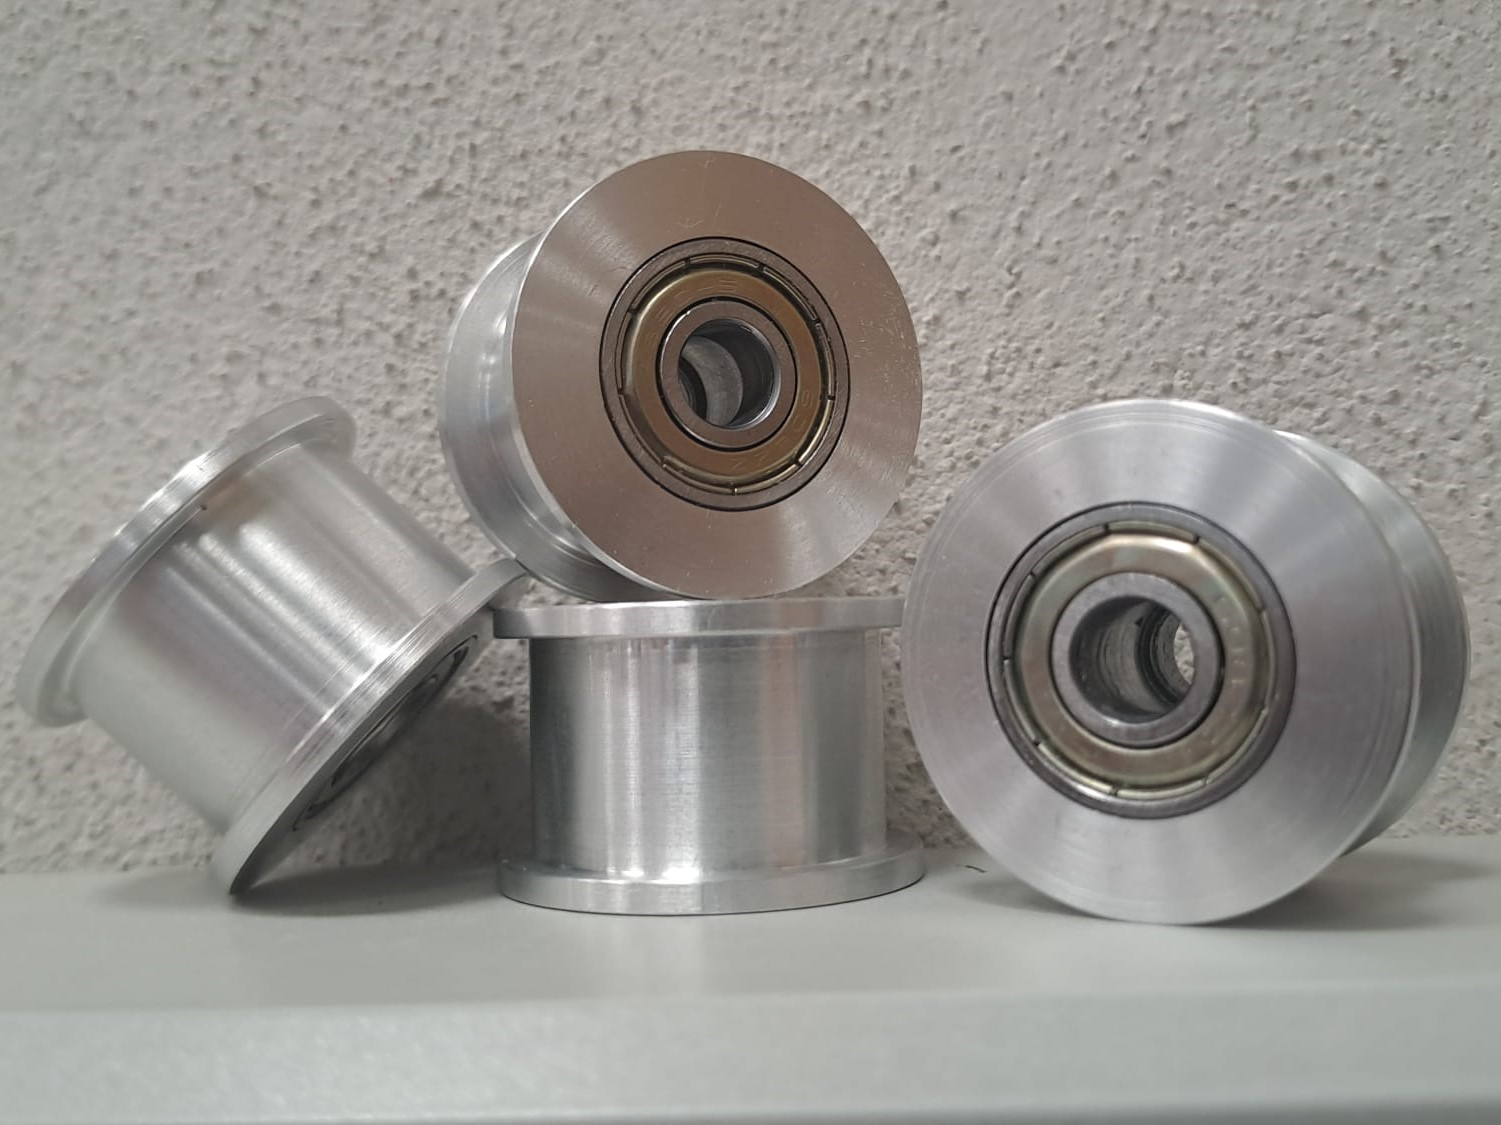
\includegraphics[width=0.9\textwidth]{Umlenkrollen_fertig.jpg}
            \centering
            \caption{Fertiggestellte \\Umlenkrollen}
            \label{ulr:f2}
        \end{subfigure}
        \caption{Umsetzung der Umlenkrollen}
        \label{ulr}
    \end{figure}

\paragraph{Distanzhülsen}\mbox{}\\
Bei den meisten V-Wheels werden Distanzhülsen zur Klemmung benötigt. Diese müssen ein sehr spezielles Maß (13.4 mm Länge) haben. Deshalb müssen Hülsen mit einer Länge von 20 mm auf diese Länge heruntergedreht werden. Dies wird mit dem rechten Eckdrehmeißel bei einer Drehzahl von 740 U/min ausgeführt. Da relativ viele solcher Teile benötigt werden, wird beim Einspannen der Drehmeißel selbst als Endstopp verwendet, um ein relativ wiederholgenaues Maß zu erhalten sowie eine simple Durchführung zu erlauben. Es wird also der Meißel auf Position gefahren und das Werkstück eingespannt, sodass es am Drehmeißel ansteht. Nun wird der Drehmeißel zurückgefahren und die Hülse kann einfach durch mehrere Plandrehoperationen, bis der Schlitten ansteht, gekürzt werden. Es muss also weder gemessen noch die Digitalanzeige verändert werden, um schnell mehrere Teile hintereinander zu fertigen.

\paragraph{Zahnscheiben}\mbox{}\\
Da die Welle des Motors recht kurz ist und die Motoraufhängung Platz wegnimmt, ist es erforderlich, die Zahnscheibe unkonventionell mit dem Motor zu verbinden. Es werden also in der Zahnriemen-Kontaktfläche zwei Löcher gebohrt, angesenkt und mit M4-Gewinde versehen, um dort 2 M4-Wurmschrauben einzuschrauben. Bei der Länge der Wurmschrauben muss darauf geachtet werden, dass sie im montierten Zustand vollständig unter der Oberfläche liegen, um den Zahnriemen nicht zu beschädigen.

\subsubsection{Aufbau}

\paragraph{Rahmen} \mbox{}\\
Gestartet wird mit der Monate des Rahmen. Hierfür werden zuerst alle Aluminiumprofile auf Länge geschnitten. Da nicht genug Profile in der Gesamtlänge des AFSS verfügbar sind, müssen teils noch Verbinder eingesetzt werden. An den Ecken werden die Profile dann mit Standardverbindungssätzen verbunden. Unten werden dann noch die Rollen montiert.

\paragraph{X-Achse} \mbox{}\\
Nachdem die Aufhängungen für die V-Slot Profile gefräßt sind, werden diese an den Rahmen angeschraubt. Auf die V-Slot Profile werden das Nivellierungssystem aufgeschraubt, dann werden die Profile an der Aufhängung befestigt. \\
Danach werden die Umlenkrollen- und die Motoraufhängungen montiert. In diese werden dann Umlenkrollen und Motoren montiert. \\




\newpage
\subsection{Software und Benutzeroberfläche}

\subsubsection{Grundlegendes}
Um dem Endnutzer die Möglichkeit zu geben, das AFSS möglichst einfach zu bedienen und die komplexe Logik der Lagersteuerung auszuführen, bedarf es eines Servers (Backend) und einer grafischen Benutzeroberfläche (GUI oder Frontend). Diese müssen eine Vielzahl an verschiedenen Funktionen beinhalten.

\subsubsection{Aufbau}
\begin{figure}[h]
    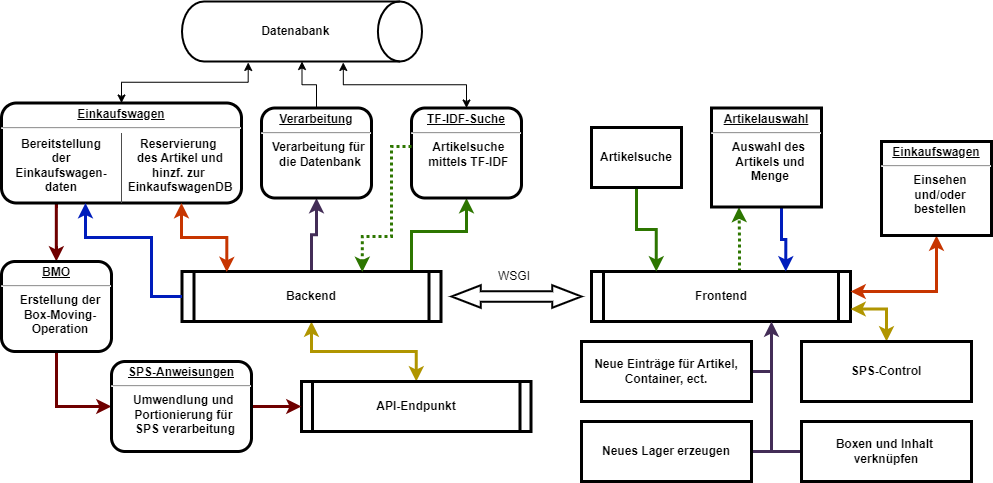
\includegraphics[width=\textwidth]{Software Howl.drawio.png}
    \caption{Gesamtüberblick des Servers}
\end{figure}

Um diesen Anforderungen gerecht zu werden, muss eine Lösung mit sehr hohem Grad an Freiheit in der Logik sowie der UI-Gestaltung gewählt werden. Weiters muss es möglich sein, dass zukünftige Schülerinnen und Schüler diese instand halten und erweitern. Aus diesen Gründen, sowie den bereits vorhandenen Kenntnissen, wird die Programmiersprache 'Python' als Grundlage des Servers verwendet.

\paragraph{Python}\mbox{}\\
Python ist eine vielseitige und hochentwickelte Programmiersprache, die für ihre Einfachheit und Lesbarkeit bekannt ist und sich sowohl für Anfänger als auch für Fortgeschrittene eignet. Sie unterstützt mehrere Programmierphilosophien, darunter objektorientierte und funktionale Programmierung, und wird in Bereichen wie Webentwicklung, Datenanalyse, künstliche Intelligenz und wissenschaftlichem Rechnen häufig eingesetzt. \cite{chatgpt}

\paragraph{Flask}\mbox{}\\
Flask ist ein leichtgewichtiges Web-Framework für Python, das durch seine Einfachheit und Flexibilität hervorsticht und sich ideal für kleinere Anwendungen oder Prototypen eignet. Es folgt einem minimalistischen Ansatz, bietet aber Erweiterungsmöglichkeiten, um komplexere Projekte zu realisieren. \cite{chatgpt}

\paragraph{Python - Virtuelle Umgebung}\mbox{}\\
Dieses Projekt enthält sehr viele externe Bibliotheken. In Python sind diese Bibliotheken mit dem Interpreter verknüpft, da bei der Installation diese externen Bibliotheken direkt beim Interpreter gespeichert werden. So kommt es jedoch dazu, dass, wenn das Programm auf einer anderen Maschine ausgeführt wird, diese Bibliotheken nicht vorhanden sind. Um Abhängigkeitskonflikte und Portabilitätsprobleme zu verringern, werden virtuelle Umgebungen verwendet. Diese enthalten den Interpreter sowie die Bibliotheken und könnten einfach auf eine andere Maschine kopiert werden.\\ Dies ist jedoch bei diesem Projekt nur bei der Entwicklung vonnöten, da es bei Fertigstellung im Docker-Container ausgeführt wird.

\subsubsection{Benutzeroberfläche}

Um die Benutzeroberfläche zu realisieren, muss eine Weboberfläche erstellt werden. Auf dieser werden alle Inhalte angezeigt, die für die Benutzung nötig sind. Sie wird vom Server zur Verfügung gestellt, sobald dieser eine HTTP-Anfrage erhält. Um diese mit eigenen Inhalten und Funktionen zu befüllen, muss dies mit HTML geschehen.

\paragraph{HTML}\mbox{}\\
HTML (HyperText Markup Language) ist die Standard-Auszeichnungssprache zur Strukturierung und Darstellung von Inhalten im Web. Sie definiert die grundlegende Struktur einer Webseite mit Elementen wie Überschriften, Absätzen, Links, Bildern und Formularen. \cite{chatgpt}\\

Dadurch, dass sich viele Elemente des UI wiederholen, wie z. B. die Navigationsleiste, bietet Flask die Möglichkeit, sogenannte 'Templates' zu verwenden. Diese können einmal definiert und dann an mehreren Teilen der Webseite verwendet werden.
Um Elemente wie Formularfelder oder Datenanzeige einfach mit den benötigten Daten anzuzeigen, gibt es die Möglichkeit, Makros zu erstellen, die von Flask mit den bestimmten Daten vorgerendert und in das restliche HTML eingefügt werden.
Um HTML, welches grundsätzlich ohne Formatierung auskommt, zu stylen, muss CSS verwendet werden.

\paragraph{CSS}\mbox{}\\
CSS (Cascading Style Sheets) ist eine Stylesheet-Sprache, die verwendet wird, um das Design und Layout von Webseiten zu gestalten. Sie ermöglicht die Trennung von Inhalt und Darstellung, indem sie Farben, Schriftarten, Abstände und andere visuelle Aspekte definiert.\cite{chatgpt}\\

Da auch Logik in der Webseite verbaut werden muss, muss zusätzlich auch Javascript verwendet werden, da HTML und CSS alleine, noch nicht gut genug mit dem Server Kommunizieren können.

\paragraph{JavaScript}\mbox{}\\
JavaScript (JS) ist eine vielseitige Programmiersprache, die hauptsächlich verwendet wird, um interaktive und dynamische Elemente auf Webseiten zu erstellen. Sie läuft direkt im Browser und ermöglicht Funktionen wie Animationen, Formularvalidierungen und die Kommunikation mit Servern in Echtzeit.\cite{chatgpt}\\

Praktisch geschieht diese Server-Kommunkation immer mithilfe diese Programmblocks:

\begin{lstlisting}[language=JavaScript]
    function sendData(data, callback) {
        var xhr = new XMLHttpRequest();
        var url = "{{url_for('main.add_stock')}}"; //Flask markup, um die richtige url zu erreichen, dies wird vor ausgabe auf der Webseite noch eingesetzt

        xhr.open("POST", url, true);
        xhr.setRequestHeader("Content-Type", "application/json");

        xhr.onreadystatechange = function () {
            if (xhr.readyState === 4 && xhr.status === 200) {
                callback(xhr.responseText)  //die funktion wir aufgerufen
            }
        };
        var jsonData = JSON.stringify(data);
        xhr.send(jsonData);
    }
\end{lstlisting}

Dieser ermöglicht die Übergabe von Daten im JSON format, und einer Funktion, die die zurückgeschickten Daten verarbeitet. In der Praxis wird dieser so aufgerufen:

\begin{lstlisting}[language=JavaScript]
function add_to_db(){
    sendData({"add_stock": {"barcode": barcode, "quantity": quant, "article": article}}, 
    set_gen_stock)
}

function set_gen_stock(req){
    document.getElementById("generated").innerHTML = req
}\end{lstlisting}

Wie im Quellcode ersichtlich, werden Daten aus der Webseite ausgelesen und in JSON konvertiert. Danach werden diese Daten zusammen mit einer Funktion an 'send\_Data' übergeben. Wie bereits erwähnt, gibt der Server dann Daten zurück. In diesem Fall werden dann Daten aus der DB vorformatiert. Diese werden dann in der zuvor übergebenen Funktion in die Webseite eingefügt.

\subsubsection{Backend}
Das Backend des Servers ist für die Datenverarbeitung verantwortlich. Es ist, wie bereits erwähnt, in Python geschrieben und stellt mit dem Flask-Framework die Benutzeroberfläche zur Verfügung. \\
Aufgebaut ist es in mehrere Bereiche: Einerseits die Webanwendung sowie die API (Application Programming Interface, Schnittstelle zwischen Anwendungen), die Anbindung an die Datenbank, die Verarbeitung der SPS-Befehle und auch der Zugriff auf die SPS.
 
%corrigiertz


\paragraph{Serverseite der Benutzeroberfläche}\mbox{}\\
In Flask könne 'bleuprints' definiert werden. Dies sind Webseitelemente die einen Bestimmten URL-Vorsatz haben. So werden anfanges 'blueprints' für Hauptfunktionen ('/', also ohne Vorsatz), Datenbankinteraktionen ('/db\_interactions') usw. definiert. Die Funktionen dafür werden dann in jeweils eigenen Dateien geschrieben. Dies ermöglicht eine weit aus bessere Übersicht bei großen Projekten. \\
Eine Funktion, die für die Verarbeitung der Anfragen einer bestimmten URL verantwortlich ist, sieht immer ähnlich aus.

\begin{lstlisting}[language=Python]
    @main.route("/add_stock", methods=["GET", "POST"])
    def add_stock():
        if request.method == "POST":
            if request.data:
                req = request.get_json()

                if "add_stock" in req.keys():
                    dt = req["add_stock"]
                    new = Stock(
                        container=db.session.query(Container)
                        .filter_by(barcode=dt["barcode"])
                        .first()
                        .id,
                        article=dt["article"],
                        quantity=dt["quantity"],
                    )
                    db.session.add(new)
                    db.session.commit()
                    return "Sucsess"

        return render_template("add_stock.html")
\end{lstlisting}  

Anfangs wird mit einem Decorator (@main.route(...)) die gewünschte URL, sowie unterstützte http-Requests definiert. Decoratoren verändern oder erweitern die Eigenschaften von Funktionen. In diesem Fall wird in der Funktion (def ...()) definiert was geschieht, wenn ein erlaubter Request an der URL 'add\_stock' eintrifft. Dieser Funktionsname kann auch in den Flask-Vorlagen verwendet werden um URLs dynamisch zu vergeben.\\
Weiters wird sortiert um welche art von Art von Anfrage es sich handelt. Bei GET-Anfragen wird typischerweise einfach nur das HTML der Webseite zurückgegeben. Bei POST-Anfragen werden zuerst die Daten dieser Anfrage eytrahiert und dann entschieden was damit gemacht werden soll. In diesem Fall wird, wenn des richtige Schlüsselwort in der Anfrage enthalten ist, ein Datenbankeintrag, mit den Daten aus dem Request, hinzugefügt. Schlussendlich wird ein Wert zurückgegeben, entweder ein HTML-Statuscode, vorgerendertes HTML oder, wie in diesem Fall, ein Text.

\subsubsection{APIs}

\paragraph{SPS - Verbindung}\mbox{}\\
Die Daten für die SPS werden in einem Ähnlichen vefahren zu verfügung gestellt. Nun schickt nicht die Benutzeroberfläche oder der Browser eine Anfrage an das Backend, sondern die SPS. Der Programmblock zur Verarbeitung dieser Anfrage sieht folgenderaßen aus:

\begin{lstlisting}[language=Python]
@api.route("/afss", methods=["GET", "POST"])
def afss():   
    request_data = {...} #aus platzgruenden verkuerzt
    if request.method == "POST":
        ... # Abfrage ob der Sender eine Siemens SPS ist
        if "next_bmos" in req.keys():
            if req["next_bmos"] == "":
                return "400"

            if is_SPS:
                return convert_instruction_for_PLC(afss_stack.get_current_bmos(int(req["next_bmos"])))

            return jsonify(afss_stack.get_current_bmos(
                int(req["next_bmos"])))

        if "inst_acknowledge" in req.keys():
            if is_SPS:
                ack = afss_stack.inst_acknowledge(
                    int(req["inst_acknowledge"]))
                if ack == "204":
                    return ack
                return convert_instruction_for_PLC(ack)
\end{lstlisting}  

Die Funktion dieses Codeblocks besteht darin, herrauszufiltern, ob eine Anfrage einer Siemens-SPS eintrifft und dann dementsprechend Daten zurückzugeben.
Wenn eine Anfrage mit dem Schlüssel 'next\_bmos' (next-box-moveing-operation) empfangen wird, wird diese dem sog. 'stack' weitergegeben, welcher diese dann verarbeitet (dies wird im Anschluss näher behandelt). Sollte diese von einer SPS kommen, werden die Zurückgeschicten Daten vorher noch so bearbeitet, dass diese von der SPS möglichst gut übersetzt werden können.
Sollte die SPS ein 'inst\_acknowledge' sowie die dementsprechenden Daten, wird im 'Stack' vermerkt dass die dementsprechende Operation bei der SPS angekommen ist.

Weiters bietet Simens auch die Möglichkeit über den Webserver der CPU auf diese zuzugreifen. Dies geschieht über das JSON-RPC Protokoll \cite{ws_s7}. Aus Testzwecken ist des durchaus nützlcih auh dierekten Zugriff auf die CPU zu haben, wenngleich es für den Normalbetrieb nicht zwingend benötigt wird. Um eine möglichst einfache bedienung zu Ermöglichen wird ein Objekt angelegt, um JSON-RPC Befehle auszuführen.

\begin{itemize}
    \item Login: Um die SPS zugreifen zu können muss erst ein Login geschehen. Hierbei werden Benutzername und Passwort benötigt, die zuerst in der SPS festgelegt wurden. Dieser führt bei Erfolg zu einem 'Session-Token', welches bei jeder folgenden Kommunikation zur Authentifizierung mitgeschickt werden muss.
    \item Daten Lesen: Die Methode 'PlcProgram.Read' gibt den Wert einer gegebenen Variable zurück.
    \item Daten Schreiben: Mit 'PlcProgram.Write' kan der Wert einer oder mehrere Variablen geändert werden.
\end{itemize}

Diese Objekt kann dann einfach in einen Anderen Programmteil importiert werden, und dort dann die Verbindung zu einer SPS herstellen. Theoretsich könnt man auch mehrere dieser Objekte anlegen, um Zugriff mehreren Steuerungen umzusetzen.

\subsubsection{Lageralgorithmus für SPS}\mbox{}\\

\begin{wrapfigure}{R}{0.6\textwidth}
    \centering
    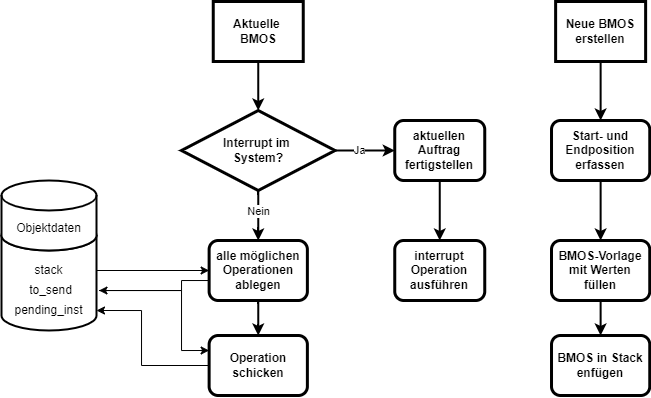
\includegraphics[width=0.52\textwidth]{stack.png}
    \caption{Diagramm der BMOS bereitstellung}
\end{wrapfigure}

Die Auftrage sind im Einkaufswagen o.ä. im Format 'Location -\> Location' hinterlegt. Um dies in eine Opeation zu zerlegen die die SPS versteht, wird eine Box-Moveing-Operation erstellt. Diese enthält alle Teilschritte, wie Schlittenposition oder Fördebandstracke, um eine Box von Position A zu Position B zu bringen. 
Die BMO wird dann in die einzelnen verwendeten Module, Förderband oder Lager, aufgeteilt und dann dem 'stack' zugeführt. Diese Instruktion enthält Daten wie:
\begin{itemize}
    \item 'instruction\_id': Eine fortlaufende Nummer um jede Anweisung zu identifizieren
    \item 'order\_id': Zusammenhängende Anweisungen, bzw. Anweisungen für die gleiche Box, haben eine gleiche Nummer
    \item 'relation': eine Liste mit 'instruction\_id's', welch vor dieser Anweisung erfüllt sein müssen
\end{itemize} 

Bei Auswahl der zu schickenden Anweisung, wird zuerst die aktuell von der SPS gemachte Anweisung vermerkt, danach weird in allen Modulen des 'stacks' nachgeschaut, welche Anweisungen jetzt ausgeführt werden können. Zu diesem Zweck wird die 'relation' einer Anweisung mit den bereits gemachten Anweisungen verglichen, wenn bereits alle relevanten Anweisungen gemacht wurden, wird der Auftrag in 'to\_send' vermerkt. Schlussendlich wird einer der in 'to\_send' vermerkten Aufträge für die SPS übersetzt und an diese geschickt. 
Wenn die SPS den Auftrag erhalten hat, schickt sie ein 'acknowledge' mit der erhaltenen ID zurück. Der Auftrag wird dann aus den 'instructions\_to\_send' gelöscht und entweder wird einfach der nächste Auftrag in 'to\_send' geschickt oder der 'BMOS' Algorithmus wird erneut durchlaufen.


\subsubsection{Datenbanken}

Als Datenbanksystem wird aufgrund des guten Supports MySQL gewählt. Dies ist ein relationales Datenbankmanagementsystem welches in einem Docker-Container aufgesetzt wird. In diesem werden alle Daten gespeichert, die zur Auswahl sowie zur Ausliferung von Teilen nötig sind.

\begin{figure}[h]
    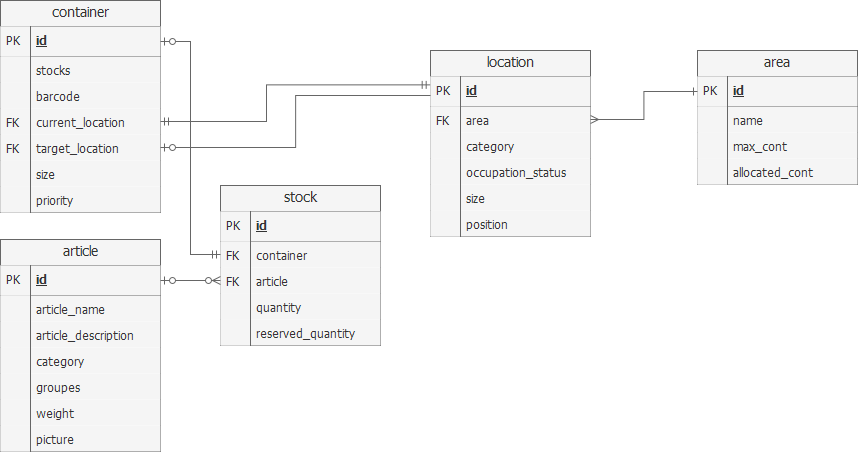
\includegraphics[width=0.6\textwidth]{DB-Schema.png}
    \centering
    \caption{Datenbankschema des AFSS}
    \label{DB-Scema}
\end{figure}

Wie in \ref{DB-Scema} ersichtlich, beinhalt diese Datenbank fünf Tabellen. Diese hohe Komplexität resultiert daraus, dass diese Struktur eine 100\%ige Flexibilität in der Ablage von Bauteilen in einem überliegendem System bietet.

Die Erste Tabelle beschreibt ein einziges theoretisches Bauteil. Dieses hat einen Namen, Gewicht, Beschreibung und Kategorien zur Filterung. Unter der Spalte 'picture' wird ein Dateiname gespeichert, der zu einem Bild zeigt, dass das Produkt abbildet.
Die zweite beschreibt einen Container. Im Lagersystem entspricht dieser einer Box. Diese kann mehrere `stocks' beinhalten, sowie durch einen Barcode identifiziert werden. Weiters muss jeder Container immer eine aktuelle Position (`current\_location') besitzen, an der die Box gerade ist. Im ausgelagerten (und noch nicht eingelagerten) Zustand ist diese `location' Position 0. Das Ziel der Box wird in `target\_location' gespeichert. Stimmt die aktuelle mit der Zielposition überein, so ist die Box an ihrem Ziel angelangt. Die Kategorie `size' beschreibt die Größe eines Containers und lässt somit theoretisch zu, dass in Zukunft auch unterschiedlich große Boxen zuverlässig in die richtigen Lagerplätze eingelagert werden. `priority' wird nicht verwendet.

Container und Artikel werden im sog. 'stock' verheiratet. Dieser kann als bauteilhaufen in einer Box verstanden werden. Es können also auch mehrere 'stocks' mit dem selben Container geben, dies würde mehreren verschiedenen Bauteilen in einem einzigen Copntainer entsprechen. Auch ist es möglich mehrere Container mit den selben 'stocks' abzubilden, welches ener aufteilung von Abuteilen auf mehrere Container entspräche.

Die Positionen der Container werden in Standorte ('locations') abgebildet. Diese entsprechen den Lagerplätzen. Sie sind einer darüberliegenden 'area' zugeordnet, welche einerseits einen Lagerschrank, aber weiters auch Module wie Vereinzelungsanalgen, abbilden kann. Standorte verfüghen weiters über eine Position welche in X, Y und Z-Richtung beschreibt, wo sich ein Standort im Referenzsystem des Lagers befindet. Auch die größe des Lagerplatzes wird abgebildet, um sicherzustellen, dass auf jeden fall nur die richtige Größe an Box eingelagert wird.


\subsubsection{Docker}

    \begin{wrapfigure}{r}{0.3\textwidth} % 'r' for right, 'l' for left
        \vspace{-20px}
        
\includegraphics[width=0.3\textwidth]{docker-logo-011.png} % Replace with your image file
        \caption{Docker-Logo: \cite{docker_logo}}
    \end{wrapfigure}

    Docker ist eine Umgebung, in der Softwareprojekte isoliert werden können. Da besonders auch bei Projekten mit großem Python anteil, viele Pakete mit verschiedenen Versoinen benötigt werden, ist es sehr hilfreich diese zu bündeln. \\
    Umgesetzt wird dies mithilfe von Containern welche einen gesamten Programmteil als alleinstehende Einheit enthält. Diese werden über ein 'Dockerfile' configuriert, welches sich im selben Ordner wie die Python-Anwendung befindet. In diesem werden Parameter wie die Python-Version und die benötigten pip-Pakete sowie den Programmeinstiegspunkt angegeben. \\ 
    Ein zweier Docker Conteianer wird mit einem MySQL-Image erstellt, dort wird die Datenbank aufgesetzt. \\
    Um diese Zwei Container miteinander Kommunizieren zu lasen, ist es ntig ein sog. docker-compose.yml File zu erstellen. Dies enthält alle Informationen über verwendete container, deren Ports, sowie Speicher für Dateien (Volumes). Bei Testbetrieb wird der Datenbankcontainer aleinstehend bestrieben und mit einem anderen Port, keine Zugriffsprobleme zu generieren. In Produktion wird dann derselbe Container in den Containerverband übertragen und dort mit einem anderen Port weiterverwendet. \\
    Erstellt wird dieser Containerverband mit den Consolenbefehlt der auf das docker-compose File zugreift. 
    \begin{lstlisting}[language=bash]
        docker build docker-compose.yml\end{lstlisting}
    Dann werden auch alle Logs in der Kommandozeile ausgegeben sowie 


\subsubsection{Artikelsuche}
\paragraph{TF-IDF und Rust Implementierung} \hspace{0pt} \\
Der TF-IDF (Term Frequency-Inverse Document Frequency) Algorithmus, ist ein Weg um wichtige wörter aus Dokumenten zu extrahieren. Er wird verwendet um beispielsweise in Suchmaschienen, eine Suchanfrage mit Webpagecontent abzugleichen, und die am besten mit der Suchanfrage übereinsteimmenden Dokumente zu sortieren. \\
Im Fall dieser Anwendung werden die Daten aus der Artikeldatenbank als 'Dokumente'  angesehen und die Suchanfrage aus dem Suchfeld wird dafür verwendet um die am besten passenden Artikel zu finden.
\\
Durch den Relativ hohen Rechenaufwand bei dieser Suchoperation wird dieser in der Programmiersprache Rust implementert. Die Implementierung in Rust ist im vergleich zu Python schon bei relativ kleinen Datenmenge bis zu 5-mal schneller.

\subparagraph{Rust}\mbox{}\\
Rust ist eine sehr effiziente und schnelle Programmiersprache die in den späten 2000er und frühen 2010ern bei Mozilla und der Open-Source-Community entwickelt. Sie unterstützt unter anderem mehr Typensicherheit und verhindert viele Programmierfehler.\cite{chatgpt}

Die Funktion dieses Algorithmus ist in drei unterteile Unterteilt.

\begin{enumerate}
    \item Term Frequenz \\
    Die Termfrequenz gibt an, wie oft ein angegebenes Wort in einem Dokument vorhanen ist. Dies wird durch die Folgende Funktion kalkuliert.
    
    \begin{lstlisting}[language=Rust]
fn term_frequency(document: &str, term: &str) -> f64 {
    // Store the lowercase document as a String to ensure it lives long enough
    let lower_document = document.to_lowercase(); 

    // Split the document into words
    let normalize_document: Vec<&str> = lower_document.split_whitespace().collect();
    // Make sure the searchterm is lowercase
    let normalize_term = term.to_lowercase();

    // Count occurrences of the term in the document
    let count = normalize_document
        .iter()
        .filter(|&&word| word == normalize_term) // Compare each word with the term
        .count();

    // Calculate the term frequency as occurrences / total number of words
    let total_words = normalize_document.len();
    if total_words == 0 {
        0.0 // Avoid division by zero if the document is empty
    } else {
        count as f64 / total_words as f64
    }
}\end{lstlisting}

    Mithilfe dieser wird eine Liste aller Wörter und der Vorkommenshäufigkeit dieser erstellt.

    \item Die zweite Komponente ist dann die Inverse Dokument Frequenz. Diese gewichtet, die Anzahl der Dokumente in dem das gesuchte Wort enthalten ist relativ zur Gesamtdokumentanzahl vorkommt. Häufig vorkommende Worte wie z.B. 'und' werden hierbei weniger gewichtet als einzigartige Wörter.

\begin{lstlisting}[language=Rust]
fn inverse_document_frequency(term: &str, all_documents: &Vec<String>) -> f64 {
    let mut num_documents_with_this_term = 0;

    // Iterate over all documents to check if they contain the term
    for doc in all_documents {
        // Normalize both term and document by converting them to lowercase
        let lower_doc = doc.to_lowercase();
        let normalized_doc: Vec<&str> = lower_doc.split_whitespace().collect();

        // Check if the term exists in the document
        if normalized_doc.contains(&term.to_lowercase().as_str()) {
            num_documents_with_this_term += 1;
        }
    }

    // Calculate IDF
    if num_documents_with_this_term > 0 {
        // Apply the IDF formula: 1 + log(total_documents / documents_with_term)
        1.0 + ((all_documents.len() as f64) / (num_documents_with_this_term as f64)).ln()
    } else {
        // If the term is not found in any document, return 1.0
        1.0
    }
}
\end{lstlisting}

    \item Nun liegt Liste davon vor, wie oft ein Wort in den Suchdaten vorkommt, als auch, wie oft ein Suchbegriff in einem bestimmten Dokument ist. \\ Als nächsten Schritt werden diese beiden Werte für jeden Suchbegriff miteinander multipliziert und ergeben somit einen Vektor der die Suchwörter in Relation zu jedem einzelnen Dokument stellt.
    \item Als letzten Schritt wird der zuvor errechnete Dokumentenvektor (der IDF jedes Suchterms in jedem Dokument) mit dem Suchvektor verglichen. Die geschieht mit der sog. Kosinus-Ähnlichkeit.
    \begin{lstlisting}[language=Rust]
fn cos_similarity(query_p: Vec<f64>, document_p: Vec<f64>) -> f64 {
    // Ensure that both vectors have the same length
    if query_p.len() != document_p.len() {
        return -1.0;
    }

    let mut dot_product = 0.0;
    let mut abs_doc_squared = 0.0;
    let mut abs_query_squared = 0.0;

    // Calculate the dot product and the magnitudes (squared)
    for i in 0..query_p.len() {
        dot_product += query_p[i] * document_p[i];
        abs_doc_squared += document_p[i].powi(2); // document_p[x] ** 2
        abs_query_squared += query_p[i].powi(2); // query_p[x] ** 2
    }

    // Calculate the magnitudes
    let abs_doc = abs_doc_squared.sqrt();
    let abs_query = abs_query_squared.sqrt();

    // Handle division by zero in case of zero vectors
    if abs_doc == 0.0 || abs_query == 0.0 {
        return 0.0;
    }

    // Return the cosine similarity
    return dot_product / (abs_doc * abs_query);
}\end{lstlisting}
    Nach der Berechnung dieser für jedes Dokument werden alle Dokumente sortiert und ja nach anforderung die benötigte Anzahl ausgegeben.
\end{enumerate}


\subparagraph{Artikelsuche nach Kategorien}\mbox{}\\
Um auche einen simpleren weg der Artikelfindung zur verfügung zu stellen, wird ausserdem die Möglichkeit implementiert, Artikel anhand von Attributen zu suchen. Zu diesem Zweck werden schon bei der Artikelerstellung Attribute für die Einträge 'Gruppen' und 'Kategorien' vergeben. In 'Gruppen' wird eine art Pfad angelegt, der die Suche eingrenzt. Beispielsweise würde so ein Eintrag folgende Daten Einthalten: ["Item", "Verbindungssatz"] enthalten. So kann bei der Artikelsuche zuerst die Überkategorie "Item" und dann die Unterkategorie "Verbindungssatz" aus mehreren verschiedenen ausgewählt werden. Um Bauteile weiter zu unterschieden, da es z.B. viele verschiedene Widerstände gibt, weren unter 'Kategorien' einzelheiten zum Produkt, wie Wert, Farbe o. ä. gespeichert.\\ 
Diese Informationen werden auch vom TF-IDF verwendet, dienen aber spezieller dazu, möglichst sicher das gewünschte Bauteil in einem Durchcklickmenue zu finden.





\newpage
\fancyhf[OHC]{
    \centering
    Vincent Sonvilla}
\fancyhf[EHC]{
    \centering
    Vincent Sonvilla}
\section{Integration und Programmierung der Steuerungstechnik \textcolor{gray}{ (Vincent Sonvilla)}}


\subsection{Aufgabenstellung}

\subsection{Tia-Portal}

Allgemeines blabla
wieso wirds verwendet oder warum --> vllt weil mix anderes verfügbar ist

    \subsubsection{Grundlagen}
    was muss man wissen um des Programm bzw. die Software bedienen zu können

    \subsubsection{Programmiersprachen}

    \subsubsection{Libraryeinbindung}
    \label{Libraryeinbindung}

\subsection{Motorenansteuerung}

\subsection{SPS-Server Kommunikation}

    \subsubsection{Zur Auswahl stehende Kommunikationsprotokolle} 
    \label{Kommunikationsprotokolle}

    Kommunikationsprotokolle ermöglichen den Datenaustausch zwischen unterschiedlichen Systemen, indem sie Standards und Regeln für die Kommunikation definieren. In diesem Projekt wurden zwei Protokolle getestet und miteinander verglichen: OPC-UA sowie das HTTP-Protokoll.


         \paragraph{Allgemeines}

        \begin{itemize}
            \item \textbf{HTTP (Hypertext Transfer Protocol):}  \mbox{} \\
            HTTP ist eines der bekanntesten Protokolle, welches für die Datenübertragung zwischen Clients und Servern verwendet wird. Es basiert auf einem Anforderungs-Antwort-Prinzip, bei dem ein Client (Bsp.: Webbrowser) Anfragen an einen Server sendet, welcher anschließend die entsprechenden Daten zurückschickt. Die Anfrage wird als HTTP Request und die Antwort als HTTP Response bezeichnet.\cite{HTTP-Allgemein}
            
            \item \textbf{OPC-UA (Open Platform Communications - Unified Architecture):} \mbox{} \\
            OPC-UA (Open Platform Communications Unified Architecture) ist ein plattformunabhängiges Kommunikationsprotokoll, das speziell für industrielle Anwendungen entwickelt wurde. Es ermöglicht eine herstellerunabhängige Kommunikation zwischen verschiedenen Geräten bzw. Systemen. \cite{OPC-UA}
        \end{itemize}

        \paragraph{Funktionsweise}

            \begin{itemize}
                \item \textbf{{HTTP (Hypertext Transfer Protocol):}} \mbox{} \\
                
            
                \item \textbf{{OPC-UA (Open Platform Communications - Unified Architecture):}} \mbox{} \\
                
            \end{itemize}
        
            

    
    \subsubsection{Verbindungsherstellung}
    Aus den in Punkt \ref{Kommunikationsprotokolle} genannten Gründen wurde das HTTP Protokoll ausgewählt. Um in TIA-Portal die Verbindung via HTTP aufzubauen, benötigt man bestimmte Libraries die von Siemens zu Verfügung gestellt werden. Diese müssen dann wie im Punkt \ref{Libraryeinbindung} gezeigt eingebunden werden, um die Funktionsbausteine der Library nutzen zu können. 

        \paragraph{Funktionsbausteine} \mbox{} \\
        In der Library stehen dann folgende Bausteine zur Verfügung:

        \begin{itemize}
            \item GET
            \item POST-PUT \\
            Mit dem POST-PUT Befehl werden Daten zum Server geschickt aber auch Daten erhalten. 
        \end{itemize}


    \subsubsection{Datenfilterung}
    Die vom Server geschickten Daten werden in einem Befehl geschickt. Aus diesem Befehl muss herausgelesen werden um welche Aufgabe es sich handelt, und die Daten die erforderlich sind um diesen Befehl auszuführen.

        \paragraph{Datenformatierung}\mbox{}\\
        Die Daten werden in einem String geschickt, welcher in zwei Teile aufgeteilt wird. Der zweite Teil ist jedoch abhängig vom ersten. \\
        
        \begin{itemize}
            \item 1.Teil: \\
            IDXXXXAXX \\
            Aus diesem Teil werden die ID-Nummer sowie der Auftrag herausgefiltert. Die ID-Nummer ist eine 4 stellige Nummer welche nach ID steht. Der Auftrag welcher ausgeführt werden muss steht in den zwei Stellen nach A.\\
            Diese werden nach folgender Codierung ausgelesen:
                \subitem 00: Kommissionierstation
                \subitem 01: Förderband
                \subitem 10: Lager 1 (Aus-/Einlagerung)
                \subitem 11: Lager 1 (Querförderer)
            \item 2.Teil: \\
            Der zweite Teil steht in Abhängigkeit zu ersten. Je nachdem welche Zahl nach A steht,also der Code welche Area angesprochen wird, ist der zweite Teil anders aufgebaut.
                \begin{itemize}
                \item 00: 
                \item 01:
                \item{10: X-Position, Y-Position, Z-Position,Ein/-Auslagerung \\
                Wobei nach jedem Symbol eine 4 stellige Zahl steht.Also X0000Y0000Z0000R0 bedeutet, dass die 
                X-Position 0, Y-Position 0, Z-Position 0 und es sich um eine Auslagerung handelt.}
                \item 11:
                
                \end{itemize}
            
        \end{itemize}

\subsection{Herausforderungen}


\newpage
\fancyhf[OHC]{
    \centering
    Nikolaj Voglauer}
\fancyhf[EHC]{
    \centering
    Nikolaj Voglauer}
\section{Elektroplanung und Realisierung \textcolor{gray}{(Nikolaj Voglauer)}}

\subsection{Elektroplanung}
\label{sec:Elektroplanung}

\subsubsection{Einleitung - Grundanforderungen}
    Die grundsätzliche Zielsetzung bei der elektrischen Planung, war die Anforderungen so zu erfüllen, dass die Lösung einerseits die Anforderungen von Erweiterbarkeit und Mobilität erfüllen und andererseits in der Schule beziehungsweise in der Werkstätte produzierbar waren. Weiterführend sollte die Umgebung im Serverschrank beachtet werden. Darunter fällt, dass die Module in die Breite von den, nur in die Tiefe verstellbaren, Profilschienen begrenzt werden.\\
    In der Anlage sollten während dem Normalbetrieb alle Komponenten vor elektrischen Störungen geschützt sein. Der Fokus liegt hierbei auf dem Schutz von Messleitungen und Steuerleitungen, an diese gibt es besonders hohe Anforderung bezüglich Präzision.\\ 
    Weiterführend sollte in der Planung stehts bedacht werden, dass die elektrischen Komponenten so verbaut werden, dass im Falle eines Fehlers sowohl Personen gut geschützt sind und dass die Geräte leicht auszuwechseln sind.\\

\subsubsection{Elektrik spezififsche Anforderungen}
\label{sec:Elektrik spezififsche Anforderungen}

    \paragraph{Versogung}\mbox{}\\
    Zur Verfügung steht dem AFSS eine 3-phasige Wechselspannung mit 400V Außenleiterspannung. Damit direkt angesteuert werden kann nur der Asynchronmotor für das Fließband. Alle anderen Elemente brauchen eine andere Spannungsebene. Die in Summe sieben Schrittmotoren brauchen 24 V mit einem möglichen Dauerstrom von über 20A. Die Logik bestehend aus Siemens-SPS mit verschiedensten Karten und einer ET200 mit Asi-Master. Diese benötigen ebenfalls 24 V und sollen getrennt versorgt werden, um bei Fehlern geschützte Logikkreise zu haben. Der Asi-Kreis benötigt eine eigene Asi-24V-Versorgung.

    \paragraph{Ansteuerungen}\mbox{}\\
    Angesteuert werden müssen 8 Motoren: 1 Asynchronmotor (250 W), 4 stärkere Schrittmotoren (2 Nm) und 3 schwächeren Schrittmotoren (40 Ncm). \\
    Der Asynchromotor soll keine Drehzahlregelung haben und über eine Wendeschützschaltung angesteuert werden. Die Schrittmotoren sollen über Schrittmotortreiber angesteuert werden. Diese Treiber werden von den PTO-Karten der SPS angesteuert.

    \paragraph{Sicherheit}\mbox{}\\
    Für die Anlage soll ein Fehlerstromschutzschalter, ein Leitungsschutzschalter, ein Motorschutzschalter und für jeden Motor eine Gleichstromsicherung ausgelegt werden.\\ 
    Um Fehler zu behandeln die potentiell von den elektrischen Schutzeinheiten nicht unterbrochen werden soll die Anlage über mehrere Not-Aus-Schalter verfügen. Zwei auf der Anlage, einer im Serverschrank/Schaltschrank und einer am Kommisionierplatz. Diese Positionierung soll es NutzerInnen ermöglichen aus jeder Position an der Anlage einen Not-Aus-Schalter zu erreichen.

    \paragraph{Bedienelemente}\mbox{}\\
    An physischen Bedienlementen sollen ein Schlüsselschalter zur Freigabe und ein dreiphasiger Drehstromschalter für eine manuelle Freischaltungsoption eingeplant werden.

    \paragraph{Schaltschrank}\mbox{}\\
    Grundsätzlich haben Schaltschränke genormte Anforderungen.\\
    Dazu gehört eine Auslegung von Kabelkanäle, die die Kabel schützen soll und Umbauten nicht zusätzlich erschweren sollen. Freifliegende Kabel sollen unter allen Umständen verhindert werden. Das Gehäuse muss geerdet sein und die inneren Komponenten vor Staub und Schmutz schützen. Bei einem potenziellen Lichtbogen soll der Schaltschrank Personen in der Nähe schützen. Zudem muss der Schrank gegen thermische Einflüsse geschützt sein, gegebenenfalls soll der Schaltschrank über eine Belüftung verfügen.\\
    Der Serverschrank schütz gegen Staub und Schutz und kommt mit einer Lüfteranlage, die die Abwärme von mehereren Gleichrichtern gut abführen kann. Zudem sind die Materialen des Schrankes vor korrosionsgeschützt.\\
    Bei der Planung muss beachtet werden, dass die Erdung aller leitungsfähigen Elemente eingehalten wird. Außerdem dürfen Umbauten wie die Montage von Rädern keine der angeführten Anforderungen widersprechen.

    \paragraph{Kabelauslegung}\mbox{}\\
    Bei den Kabeln gibt es mehrere Punkte, die beachtet werden müssen beim Auslegen. Während Spannungsabfall bei den Längen des AFSS vernachlässigt, werden können muss besonders auf Schleppkettentauglichkeit geachtet werden. Steuer- und Messkabel müssen entsprechend geschirmt werden und entsprechend dem Strom muss der Querschnitt gewählt werden. Dabei sind die Querschnitte aber auch stark abhängig von den Schutzeinheiten im Schaltkreis.

    \paragraph{Module}\mbox{}\\
    Die Paneele/Module, auf welchen die elektrischen Komponenten montiert werden sollen, müssen ebenfalls alle Erdungserwartungen erfüllen und mechanisch den Belastungen standhalten. Dabei ist das Gewicht die beachtlichste Belastung. Eine gerechte Drahtverlegung muss gewährleistet sein und die Modularität der Paneele soll vorteilhaft ausgenutzt werden und sollen nicht das Projekt unnötig verkomplizieren. Kostentechnisch soll dabei ein möglichst billiges, aber standhaftes Material gewählt werden.

\subsubsection{Mechanische Planung}

    \paragraph{Modulprinzip}\mbox{}\\
    Es wurden bereits die Anforderungen an die Module beschrieben. Doch es gäbe noch weitere Alternativen für den Innenraum des Serverschrankes, so könnte man eine große Platte verwenden und diese an die Profilschienen festschrauben. Eine weitere Option wäre eine plattenlose, dabei würde man die Hutschienen direkt auf die Profilschienen des Serverschrankes montieren.\\
    Die große Platte entfällt als Möglichkeit insofern, da diese nicht in der Schule produzierbar gewesen wäre. Die plattenlose Option wäre eine kosteneffiziente Möglichkeit, allerdings gibt es viele Elemente, die im Schaltschrank nicht auf Hutschienen montiert werden können, diese bräuchten immer eine Montageplatte.\\
    Damit ein einheitliches Design eingehalten werden kann, haben wir uns für das Modulprinzip entschlossen. Dieses ermöglicht es Elementen, die für Hutschienen ungeeignet sind, wie dem 24V-ASI-Gleichrichter, montiert zu werden und ist weiterhin in der Schule produzierbar.

    \paragraph{Platten-Material}\mbox{}\\
    Für die Materialwahl gab es zwei realistische Möglichkeiten. Die Modulplatten hätten vollständig aus Aluminium gefräst werden können oder aus Dibond. Die Aluplatten bieten den Vorteil der Leitfähigkeit und somit müsste man nur die Platte erden und die Elemente auf der Platte wären alle dementsprechend geerdet. Doch Aluminium ist teuer und ein wertvoller Werkstoff, da ein umsichtiger Umgang mit Ressourcen wichtig ist wurden dann doch die Dibond-Platten als Projektstandard definiert. Diese sind zwei dünne Platten aus Aluminium die auf einen Kunststoff aufgepresst werden. Dibond bietet keine elektrische Leitfähigkeit, folglich müssen alle Elemente zusätzlich geerdet werden. 

    \begin{figure}[H]
        \centering
        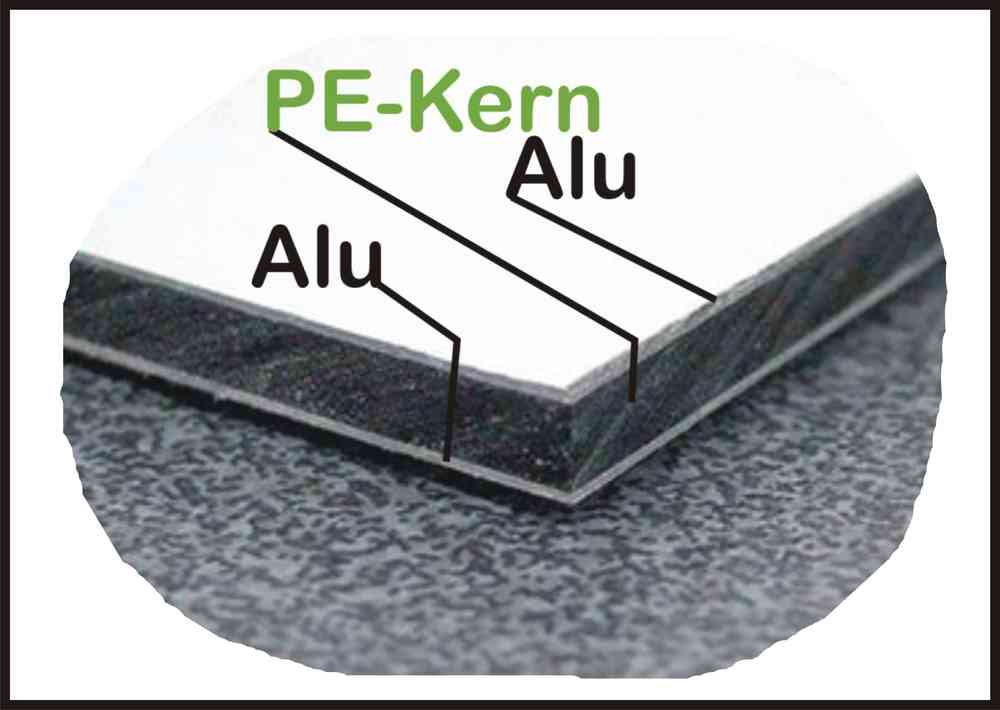
\includegraphics[width=0.5\textwidth]{Dibond_Platten_ml.jpg}
        \caption{Dibond-Platte, Quelle: \cite{Dibond-Platte}}
        \label{fig:Dibond}
    \end{figure}
        
    \paragraph{Digitaler Zwilling}\mbox{}\\
    Moderner Schaltschrankherstellung begenen im Herstellungsprozess oft große logistische Probleme. Jeder Prozessschritt ist eine Fehlerquelle und wenn Fehler nicht früh erkannt werden plfanzen sich diese fort. Damit zwischen den Prozessschritten keine Kommunikationsprobleme entstehen setzen viele Hersteller auf das Prinzip des digitalen Zwillings.\\
    Dieser im Grunde ein digitaler Schaltschrank, welcher im ersten Prozessschritt, der Planung, ausgeplant wird und im Herrstellungsprozess, sei es der Schrankbau oder die Bestückung, wird einerseits immer derselbe digitale Zwilling aktualisiert und aber auch referenziert. Das heißt alle Prozessschritte beziehen sich auf den selben Plan bzw. digitalen Zwilling (siehe \ref{fig:digilaerZwilling}).\\

    \begin{figure}[H]
        \centering
        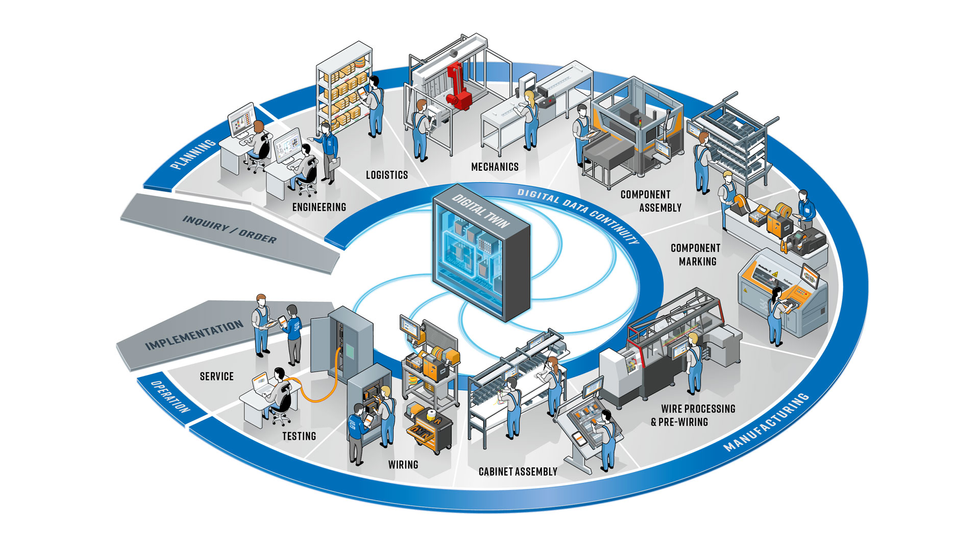
\includegraphics[width=1\textwidth]{Cabinet-Building-Komax-SCB-Component-Printer.png}
        \caption{Digitaler Zwilling, Quelle: \cite{digitaler_zwilling_bild}}
        \label{fig:digilaerZwilling}
    \end{figure}
    
    Es setzt ein breites Feld an Firmen auf dieses Prinzip. Firmen wie Weidmüller, Komax, Steinhauer und noch viele mehr haben eine Firmenzusammenarbeit die ohne einen digitalen Zwilling nicht möglich wäre\cite{smart_cabinet_building}.In diesem Fall werden die jeweiligen Prozessschritte meistens von einer neuen Firma übernommen, in diesem Bündnis ist der digitale Zwilling der Schlüssel zum Erfolg. Mann kann dieses Prinzip der Dokumentation bzw. Planung als Industriestandard verstehen.\\
    Um den Prozesss der Herstellung des Schaltschrankes möglichst nahe an die Praktiken aus der Industrie anzugleichen wird auch der Schaltschrank des AFSS mithilfe eines digitalen Zwillings geplant. Dieser wird in Fusion360 gezeichnet und soll den Sollzustand des Schaltschrankes abbilden.\\
    Um den die Konstruktion anzufangen braucht es eine möglichst ausführliche Ausmessung des bereits bestehenden Serverschrankes. Besonders wichtig sind die Elemte die direkt am Umbau beteiligt sind, wie die Profilschienen, die Türen und die Lüfter.\\

    ----
    Tabelle in Anhang einfügen mit abmessungen und Bildern    
    Wie fängt man einen digitalen Zwilling an?
    -Abmessungen: Alle Abmessungen die gemacht wurden anführen

    -Serverschrank in CAD Nachzeichnen: Dabei beschreiben was besonders wichtig ist, sowie das Bewegliche Teile in echt auch beweglich sein müssen in Fusion360. WIe waren die Schritte die beim Zeichnen gemacht wurden, mit was ich anfange.

    -Module: Ist der Schaltchrank fertig übernommen aus der realität kann man anfangen mit einem Modul. Dabei fällt einem zum Beispiel schon eine sache auf, sowie die Tatsache, dass wenn man die Profilschinen an der selben Position lässt würden sich die Türen nicht schließen lassen. Folge daraus ist, die Profilschinen müssen verschoben werden. Der Aufbau des Serverschranks lässt dies zu.

    -Weitere Module: diese werden dann auch in Fusion360 gezeichnet und dann in den digitalen Zwilling eingefügt. Dabei kann man schön erkennen wie die Module Anneinander gereiht gehören, welche Reihenfolge sinnvoll ist und ob sich die Menge an Elektrischen Einheiten auch ausgeht mit den Modulen. 

    -Dieser soll auch immer die akktuelle version abbilden


\subsection{Realisierung}
\label{sec:Schaltplan}





\newpage
\fancyhf[OHC]{
    \centering
    Elena Widmann}
\fancyhf[EHC]{
    \centering
    Elena Widmann}
\section{Sensorik und Sicherheitstechnik \textcolor{gray}{(Elena Widmann)}}

\subsection{Aufgabenstellung}

\subsection{Sensorik}

\subsubsection{Endschalter}
Beim Verplanen der Endschalter ist zwischen Software- und Hardware-Endschalter zu unterscheiden. Die Software-Endschalter begrenzen den Arbeitsbereich der Achse und sollten innerhalb des Bereichs der Hardware-Endschalter parametriert werden. Ihre Positionen werden direkt im Siemens TIA-Portal eingestellt und können falls notwendig einfach auf die aktuelle Geschwindigkeit angepasst werden. Werden die Software-Endschalter angefahren, wird der Technologiealarm 533 ausgelöst, und die Dynamikwerte werden gestoppt, das Technologieobjekt bleibt hierbei freigegeben. Werden sie jedoch überfahren wird das Technologieobjekt gesperrt. \\
Die Hardware-Endschalter begrenzen den maximal zulässigen Verfahrensbereich der Achse. Bei ihnen wird nicht unterschieden, ob die Endschalter angefahren oder überfahren werden. Beim Anfahren der Schalter wird der Technologiealarm 531 ausgelöst. Er sperrt das Technologieobjekt und muss, bevor der Auslösebereich der Hardware-Endschalter wieder verlassen werden kann, quittiert werden. \cite{axis_manual}\\
Auf jeder der drei Achsen des AFSS, und auf dem Querförderer, müssen Hardware-Endschalter montiert werden. Die Auswahl begrenzte sich hierbei auf die uns zur Verfügung gestellten Sensoren, welche unter Berücksichtigung ihrer Funktion auf den verschiedenen Positionen eingebaut wurden.

\paragraph{Positionsschalter mit Rollhebel} \mbox{}\\
An der x-Achse werden als Hardware-Endschalter Positionsschalter mit Rollhebel verwendet (siehe Abb. \ref{roll_sens}). Von den insgesamt vier Stück werden zwei an der unteren und zwei an der oberen x-Achse befestigt. Davon besitzen drei jeweils einen Öffner- und einen Schließerkontakt \cite{schmersal_3}, wohingegen einer der Endschalter aus zwei Öffnerkontakten besteht \cite{schmersal_1}. Um Einheitlich zu bleiben, und da es sicherheitstechnisch auch von Vorteil ist (Drahtbruchsicherheit), verwenden wir jeweils einen der Öffnerkontakte der Endschalter. Zum Schalten des Rollhebels der Positionsschalter müssen auf dem x-Schlitten der oberen sowie unteren x-Achse Auslöser angebracht werden. Diese befinden sich mittig auf der Seite der Sensoren und gleichen einem vom Schlitten abstehenden Arm, welcher sich aus gestapelten, mit dem Lasercutter gefertigten, Teilen zusammensetzt.

\paragraph{Induktive Endschalter} \mbox{}\\
Als Hardware-Endschalter an der y-Achse werden induktive Sensoren verwendet (siehe Abb. \ref{ind_sens}). Davon werden zwei an der unteren und zwei an der oberen Seite der y-Achse befestigt, also auch hier wieder insgesamt vier Sensoren. Sie funktionieren so, dass durch eine Spule ein Magnetfeld erzeugt wird, welches dann in einem sich dem Sensor frontseitig nähernden elektrisch leitendem Material Wirbelströme erzeugt. Dadurch verändert sich das Magnetfeld und die Kontakte des induktive Sensors werden über einen Schmitt-Trigger geschaltet. Die Sensoren besitzen jeweils einen Öffner- und einen Schließerkontakt, wir verwenden jedoch ersteres um Drahtbruchsicherheit zu gewährleisten. Damit die induktiven Sensoren korrekt auslösen können, müssen auf dem Shuttle der y-Achse elektrisch leitende Gegenstücke angebracht werden.

\paragraph{Endtaster} \mbox{}\\
An der yz-Achse werden vier und am Querförderer zwei Stück mechanische Endtaster als Endschalter verwendet. Auf einem Endtaster befindet sich ein Schließerkontakt in Form eines Tasters, welcher durch anfahren geschalten wird (siehe Abb. \ref{tast_sens}). Zum Betätigen der Taster müssen sich Auslöser auf dem Shuttle und den Seiten der Querfördererstation befinden.\\

\begin{figure}[H]
    \centering
    \begin{subfigure}{.3\textwidth}
        \centering
        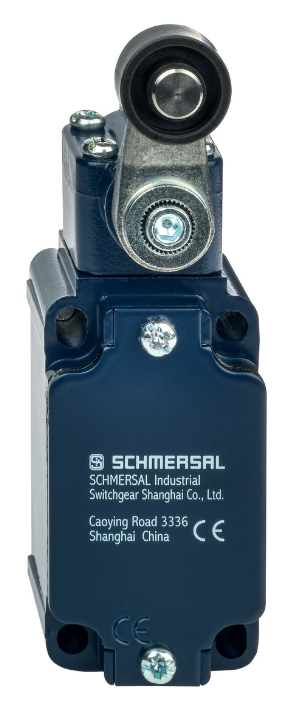
\includegraphics[width=0.5\textwidth]{Sensors/Rollendschalter.png}
        \caption{Rollendschalter \cite{schmersal_pic}}
        \label{roll_sens}
    \end{subfigure}%
    \begin{subfigure}{.3\textwidth}
        \centering
        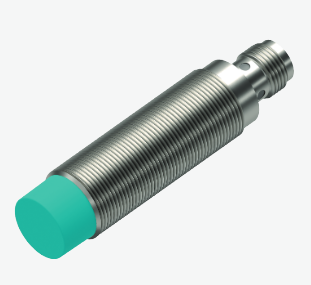
\includegraphics[width=1\textwidth]{Sensors/Induktiver_Sensor.png}
        \caption{Induktiver Sensor \cite{induktiv_sensor}}
        \label{ind_sens}
    \end{subfigure}%
    \begin{subfigure}{.3\textwidth}
        \centering
        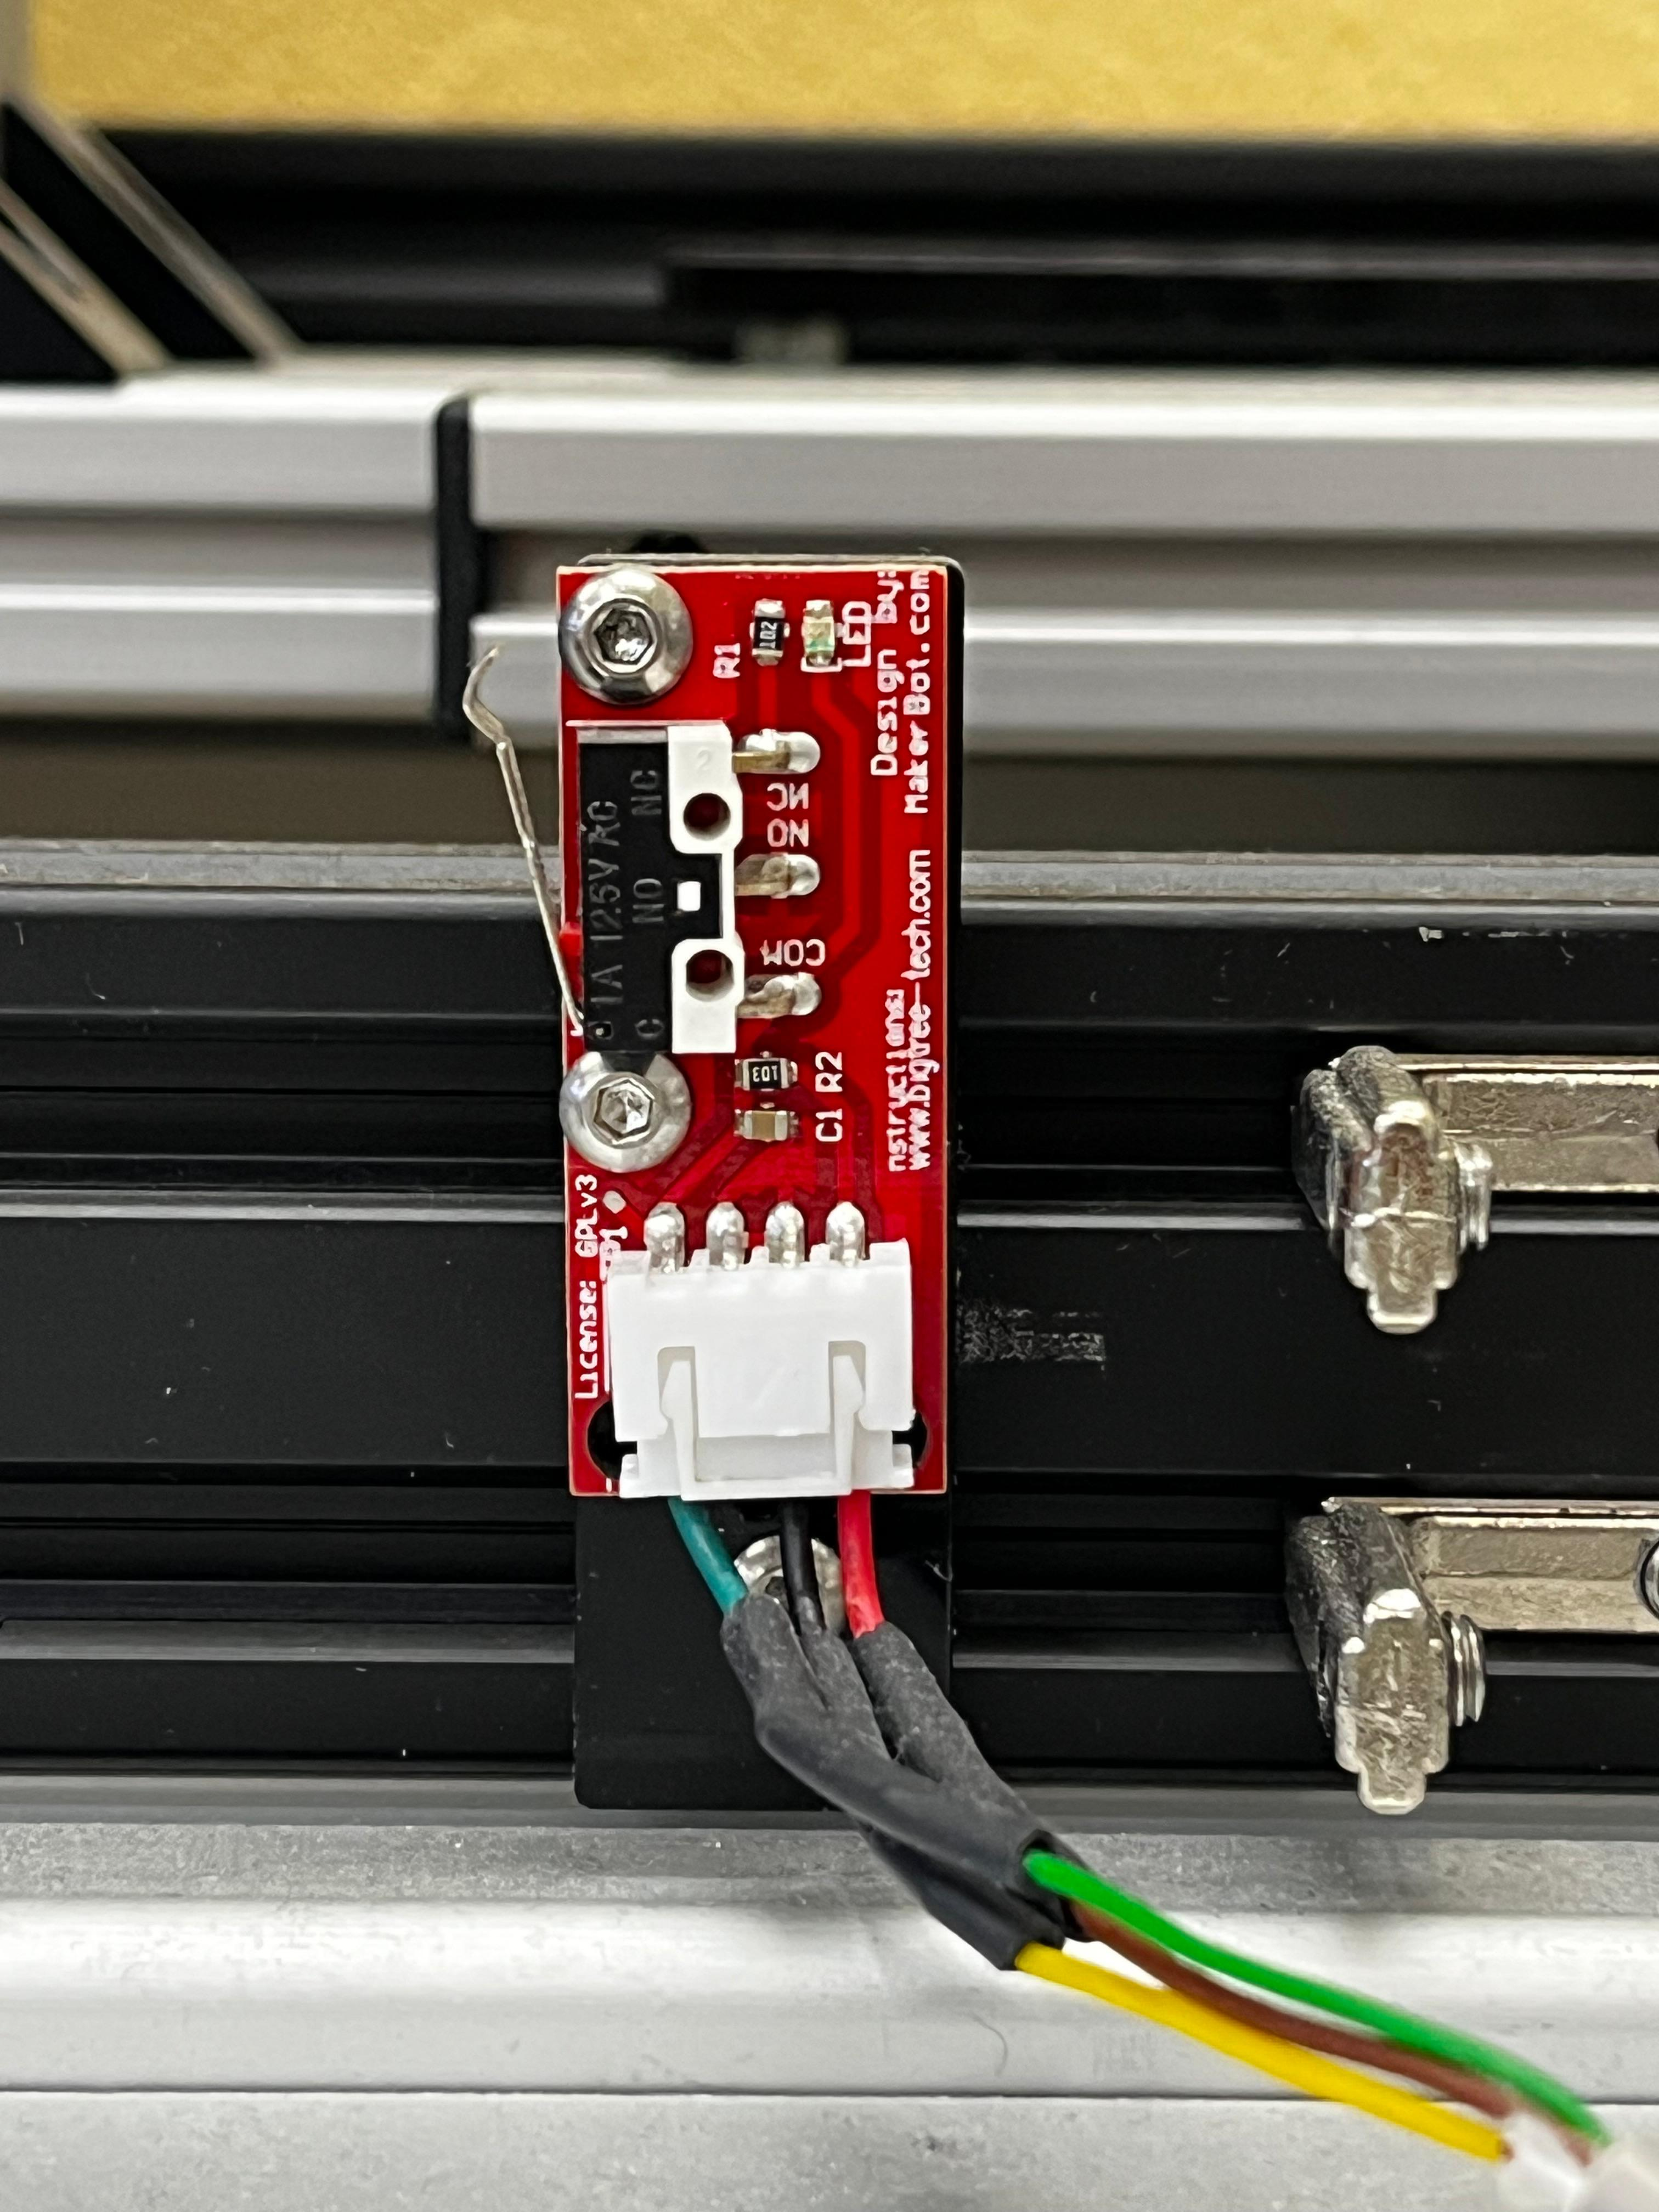
\includegraphics[width=0.9\textwidth]{Sensors/Endtaster.jpg}
        \caption{Endtaster}
        \label{tast_sens}
    \end{subfigure}
    \caption{Endschalter}
    \label{ulr}
\end{figure}

\subsubsection{Referenztaster}
Um die Motoren auf die richtige Position fahren zu können, müssen diese an allen drei Achsen und am Querförderer referenziert werden. Somit wird verhindert, dass bei einem Neustart des Systems sich die Koordinaten der Positionen, auf denen sich die Bauteilboxen befinden, nicht verändern und es zu keiner Kollision zwischen Shuttle und einer Box bzw. dem Gerüst kommt.\\
Zum Referenzieren müssen Sensoren an den Achsen und am Querförderer angebracht werden, welchen den jeweiligen Nullpunkt angeben. Hierfür werden Opto Interrupter verwendet, da diese einfach durch anfahren ausgelöst werden können. In einem Opto Interrupter befindet sich eine LED, dessen Lichtstrahl auf einen Photo Transistor trifft. Dieser schaltet daraufhin durch und es liegt eine Spannung am Emitter an. Wird jetzt jedoch der Lichtstrahl der LED unterbrochen, sperrt der Transistor und es fließt kein Strom. Bei der SPS-Programmierung ist daher zu beachten, dass sich der Ausgang des Sensors im nicht geschalteten Zustand auf HIGH befindet. Wird der Lichtstrahl jedoch unterbrochen, liegt am Sensorausgang keine Spannung an und der Eingang der SPS erhält ein LOW Signal.\\
Damit während eines Referenziervorgangs der Lichtstrahl der LED unterbrochen wird und der Referenztaster auslöst, müssen auch hier wieder Auslösevorrichtungen an den beiden x-Schlitten, am Shuttle und an der Querfördererstation angebracht werden.\\
In unserem Fall werden TP808 zum Referenzieren verwendet. Hierbei ist zu beachten, dass die sich darin befindende Diode nur mit einer maximalen Flussspannung von \qty{1.35}{\volt} betrieben werden darf.\cite{TP808} Da die Opto Interrupter jedoch über ASi-Bus mit der SPS verbunden werden, welche eine Spannung von \qty{24}{\volt} liefert, musste eine eigene Platine entworfen und gelötet werden, um das Bauteil nicht mit einer zu hohen Betriebsspannung zu zerstören. Hierfür wurde die Software Fusion360 verwendet, welche das Designen von Leiterplatten ermöglicht. Hergestellt wurden diese dann durch unsere eigene schulinterne Leiterplattenfertigung. Insgesamt musste die Referenzplatine sieben mal hergestellt werden.

\paragraph{Schaltungsentwurf} \mbox{}\\
Die Schaltung sollte so konzipiert werden, dass keines der involvierten Bauteile über längeren Normalbetrieb oder durch kurzzeitige hohe Ströme bzw. Spannungen, beschädigt wird. Das Ziel ist, die korrekte Funktion des Opto Interrupters auch zukünftig noch sicher stellen zu können. Dafür ist besonders wichtig auf dessen elektrische Eigenschaften zu achten, welche im Datenblatt zu finden sind. Für den fertigen Entwurf der Schaltung siehe Abb.\ref{Ref_Schaltplan}\\
Im Opto Interrupter befindet sich eine LED mit einer maximalen Durchlassspannung von \qty{1.35}{\volt}. und einer typischen Durchlassspannung V$_{F}$ von \qty{1.2}{\volt}. Um diese nicht mit den vollen \qty{24}{\volt} der Betriebsspannung V$_{B}$ zu überlasten muss ein Vorwiderstand R$_{1}$ eingebaut werden. Um die LED zum leuchten zu bringen, soll ein minimaler I$_{F}$ von \qty{10}{\milli\ampere} fließen. Dann lässt sich daraus der Vorwiderstand aus dem ohmschen Gesetz und mit Hilfe der Maschenregel berechnen:

\begin{equation*}
    R_{1} = \frac{V_{B} - V_{F}}{I_{F}} = \frac{\qty{24}{\volt} - \qty{1.2}{\volt}}{\qty{10}{\milli\ampere}} = \qty{2.28}{\kilo\ohm}
\end{equation*}

In der HTL wir den Schülerinnen und Schülern die Widerstandsreihe E12 zur Verfügung gestellt. Daher wird in der Schaltung der nächstgrößere Widerstand mit dem Wert $\qty{2,7}{\kilo\ohm}$ verwendet.\\
Der Phototransistor, welcher als Gegenstück zur LED dient, darf mit einer maximalen Collector-Emitter-Spannung von \qty{30}{\volt} betrieben werden, wodurch er gut geeignet ist für das Ziel der Schaltung. Um jedoch im besten Fall die gesamten \qty{24}{\volt} für den Eingang der SPS an der Klemme X1 abgreifen zu können, wird ein Spannungsteiler verwendet, bei dem nach dem Transistor ein Widerstand R$_{3}$ parallel zur Klemme X1 eingebaut wird. Da nur ein niedriger Strom benötigt wird, kann I$_{R3}$ relativ klein sein, hier \qty{1}{\milli\ampere}. Daraus lässt sich dann der Widerstandswert wie folgt berechnen:

\begin{equation*}
    R_{3} = \frac{V_{B}}{I_{R3}} = \frac{\qty{24}{\volt}}{\qty{1}{\milli\ampere}} = \qty{24}{\kilo\ohm}
\end{equation*}

Auch hier wird wieder der nächstgrößere Widerstandswert, der zur Verfügung gestellt wird, verwendet. R$_{3}$ entspricht somit dem Wert $\qty{27}{\kilo\ohm}$.\\
Für Funktionstests und die Inbetriebnahme ist es wichtig, dass eine Möglichkeit gegeben ist, den Zustand des Ausgangs der Schaltung anzuzeigen. Hierfür wird eine grüne 5mm LED verwendet, welche parallel zur Klemme X1 eingebaut wird. Da der Transistor einen maximalen Collector Strom von \qty{20}{\milli\ampere} besitzt, wurde die Entscheidung getroffen, die grüne LED nur mit \qty{10}{\milli\ampere} zu versorgen, da diese auch bei geringerem Strom genug Leuchtkraft für den benötigten Zweck besitzt. Bei einem Strom I$_{R2}$ von \qty{10}{\milli\ampere} besitzt die LED einen Spannungsabfall V$_{LED}$ von \qty{2.1}{\volt}.\cite{led_grün} Daraus lässt sich dann er Widerstand R$_{2}$ berechnen:

\begin{equation*}
    R_{2} = \frac{V_{B} - V_{LED}}{I_{R2}} = \frac{\qty{24}{\volt} - \qty{2.1}{\volt}}{\qty{10}{\milli\ampere}} = \qty{2.19}{\kilo\ohm}
\end{equation*}

Der nächsthöhere Widerstand der E12 Reihe entspricht $\qty{2,2}{\kilo\ohm}$, um auf Nummer sicher zu gehen wird jedoch der um eine Stufe größere Widerstand mit einem Wert von $\qty{2,7}{\kilo\ohm}$ verwendet. Wenn der Lichtstrahl im Opto Interrupter nicht unterbrochen wird und der Transistor somit durchschaltet, leuchtet die grüne LED. Wird jetzt der Lichtstrahl unterbrochen erlischt die LED. Damit diese nicht während des Normalbetriebs dauerhaft leuchtet wird ein Jumper eingebaut, mit welchen die LED ganz einfach aus der Schaltung ausgeschlossen werden kann.

\begin{figure}[H]
    \centering
    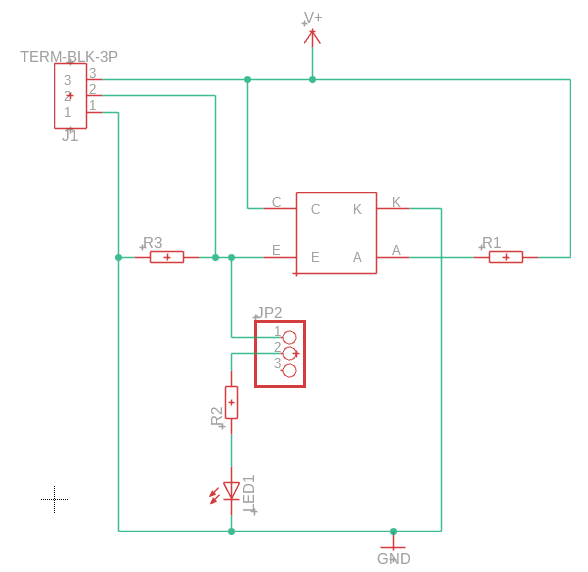
\includegraphics[width=0.6\textwidth]{Sensors/Ref_Schaltplan.png}
    \caption{Schaltplan Referenzplatine}
    \label{Ref_Schaltplan}
\end{figure}

\paragraph{Platinenentwurf und -herstellung} \mbox{}\\
Um die benötigten Referenzplatinen herstellen zu können, muss zuerst ein Leiterplattenplan in Fusion360, ehemals Eagle, erstellt werden. Über den Sharepoint der HTL lässt sich eine Elektronikbibliothek, die alle in der Schule verfügbaren Bauteile beinhaltet, herunterladen. Da der in der Schaltung verwendete Opto Interrupter nicht in der Schule verfügbar ist, sondern extern organisiert werden musst, befindet er sich nicht in dieser Elektronikbibliothek. Daher muss für ihn ein eigenes Symbol sowie ein dazugehöriger Footprint gezeichnet werden.\\
Zum Entwerfen des Printed Circuit Boards (PCB) muss ein neuer Elektronikentwurf in Fusion erstellt werden. Hier muss zuerst der zugehörige Schaltplan gezeichnet werden. Wichtig ist, dass bei der dreipoligen Schraubklemme das Bauteil 3282837-3 (J1) verwendet wird, da sonst die Abstände zwischen den Lötpads zu klein und diese zu nah bei einander sind. Damit der Jumper (JP2) nicht verloren geht, wenn die Verbindung zwischen Ground und LED aufgehoben werden soll, wird ein dreipoliger Pinheader verwendet, um den Jumper für den gegebenen Zeitraum einfach umstecken zu können.\\
Nach Fertigstellung des Schaltplans kann in Fusion ein passendes Leiterplattendokument erstellt werden, welches die Bauteile und die zugehörigen Verbindungen direkt übernimmt. Für den fertigen Leiterplattenplan des Referenztasters siehe Abb.\ref{Ref_LPPlan}. Da beim verwendeten Opto Interrupter Löcher zur Montierung vorhanden sind, müssen auf der Platine selbst keine zusätzlichen Bohrungen eingeplant werden. Bein der Anordnung der Bauteile auf der Platine ist zu beachten, dass sich die Löcher am Opto Interrupter, am schmäleren rand der Platine befinden. Um eine leichtere Verkabelung zu ermöglichen, sollte auch die Schraubklemme am Rand der Platine platziert werden.

\begin{figure}[H]
    \centering
    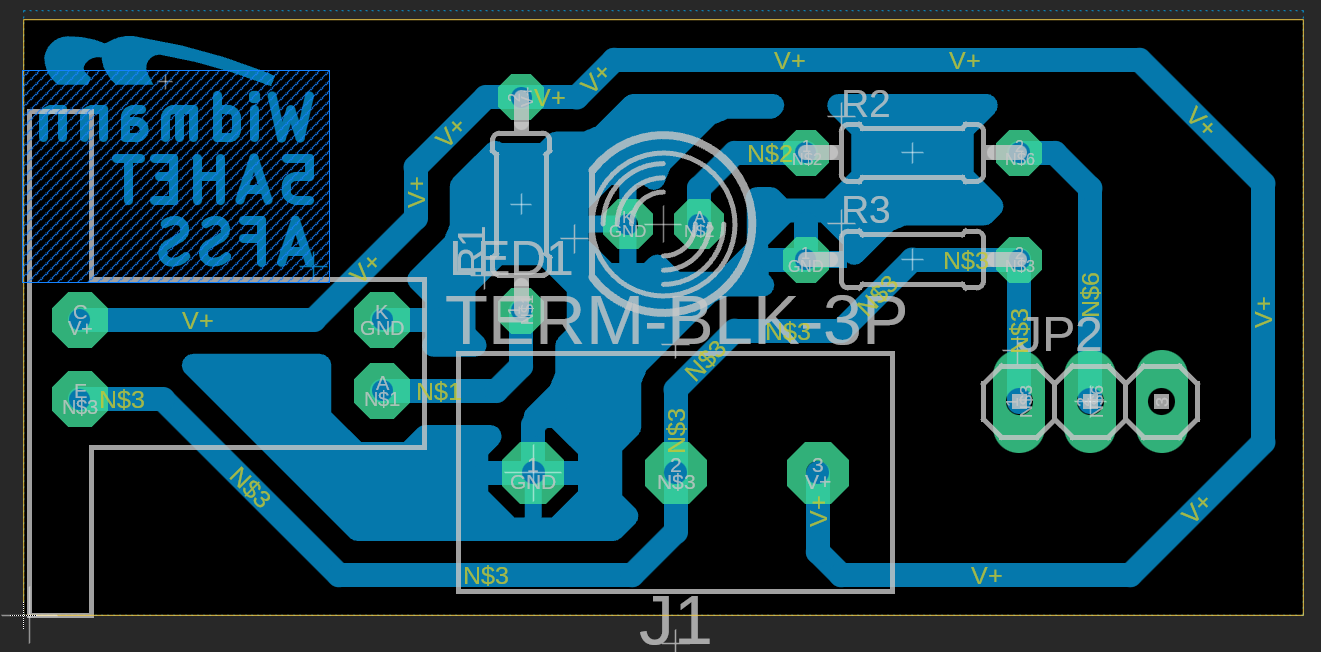
\includegraphics[width=0.7\textwidth]{Sensors/Ref_Leiterplattenplan.png}
    \caption{Leiterplattenplan Referenzplatine}
    \label{Ref_LPPlan}
\end{figure}

Wenn die Bauteile alle platziert und verbunden worden sind, sowie ein Polygon über die gesamte Platine gezogen worden ist, muss diese noch auf Fehler geprüft werden. Auch hier ist eine bereits fertige Datei, welche die benötigten Design Rules für Fusion360 beinhaltet, auf der Schulwebsite zu finden. Wichtig ist, damit die Platine zur Produktion in der Leiterplattenfertigung der HTL eingereicht werden kann, muss diese den vorgegebenen Anforderungen entsprechen. Dazu gehört, dass sich das HTL-Logo auf der Platine befindet und die Texteinstellungen Font: Vector, Ratio: \qty{16}{\percent} und Size: min \qty{70}{mil} entsprechen. Auch die Breite der Kupferbahnen darf nicht zu klein sein (hier: \qty{32}{mil}).\\
Nach Einreichung des Fertigungsauftrags wird die Platine von Schülerinnen und Schülern der HTL gefertigt. Der Prozess startet mit dem Reinigen des Basismaterials, um es daraufhin mit dem Negativtrockenresist (Trockenfilm) zu laminieren. In den nächsten Schritten werden die Layout-Informationen mit einem Belichter auf das Laminat übertragen und das unbelichtete Laminat mit einer Natrium-Carbonat Lösung von der Platine entfernt. Daraufhin werden durch Ätzen mit einer Eisen-III-Chlorid-Lösung strukturierte Kupferflächen freigestellt. Als Nächstes werden die Löcher in die Kupferpads gebohrt und die Platine auf ihre korrekte Größe zugeschnitten. Durch das Legen der Leiterplatte in eine Entschichtlösung aus \qty{5}{\percent}{igem} Kaliumcarbonat mit Wasser werden Ätzresiste von der Platine entfernt. Zu guter Letzt wird die Platine mit einem Versiegelungslack versiegelt, um sie vor Umwelteinflüssen und Korrosion zu schützen.

\paragraph{Platinentestung und Messung} \mbox{}\\
Um die korrekte Funktionsweise der Referenzplatine sicher zu stellen, muss diese nach dem Löten getestet werden. An der Klemme X1 wurden Spannungswerte zwischen \qtyrange{19.7}{21.3}{\volt} gemessen. Obwohl die Spannungen unter den gewünschten \qty{24}{\volt} liegen können die Platinen problemlos verwendet werden, da die verwendeten AS-i-Slaves einen minimalen HIGH-Eingangsschaltpegel von \qty{10}{\volt} besitzen.\cite{AS-i-Slave}

\subsubsection{Lichttaster}

\subsubsection{Barcode-Scanner}
\begin{wrapfigure}{R}{0.34\textwidth}
    \vspace{-20px}
    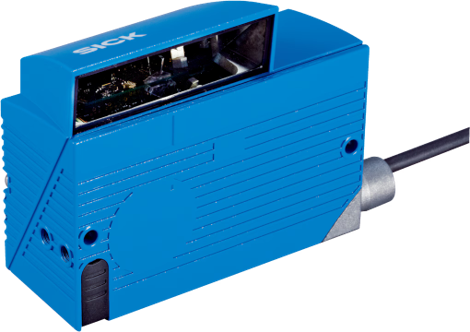
\includegraphics[width=0.34\textwidth]{Sensors/Barcodescanner.png}
    \caption{Barcodescanner CLV61x-2Port}
    \label{BarScan}
\end{wrapfigure}

Durch anbringen eines sich nicht wiederholenden Barcodes auf jeder Box wird eine gute Möglichkeit geschaffen, in der Software den Behälter und die sich darin befindenden Bauteile einander zuzuordnen. Unter der Voraussetzung, dass die Benutzerinnen und Benutzer vor jeder Wiedereinlagerung ihrer Box zuerst dessen Barcode einscannen, wird die Wahrscheinlichkeit, dass der Lagerplatz einer Box falsch abgespeichert wird, verkleinert. Somit sinkt die Chance, dass bei Bestellen eines Bauteils die falsche Komponente geliefert wird. Das erfassen des Barcodes findet mittels eines Barcodescanners der Firma SICK statt (siehe Abb.\ref{BarScan}), welcher bei der Kommissionierstation untergebracht ist, um eine einfache Bedienung gewährleisten zu können.\\
Der uns zur Verfügung gestellte Barcodescanner (CLV61x-2Port) ist in der Lage alle gängigen Codearten einzulesen.\cite{Barcodescanner} Barcodes wurden so entwickelt, dass bereits beim Einlesen erkannt wird, wo dieser anfängt und aufhört, damit beim einscannen nicht auf die richtige Ausrichtung geachtet werden muss.

\paragraph{Einbindung ins TIA-Portal \cite{BarScan_Handbuch}}\mbox{}\\
Damit der eingelesene Barcode an den Webserver weitergegeben werden kann, muss dieser im Siemens TIA-Portal abgespeichert werden. Mit der CPU verbunden wird der Scanner über PROFINET. Hierbei handelt es sich um einen auf Industrial Ethernet basierenden Kommunikationsstandard und eine Weiterentwicklung des PROFIBUS Vorgängers. Über ihn lässt sich die gescannte Nummer ganz einfach an die SPS übermitteln.\\
Im TIA-Portal Projekt muss, um eine Verbindung zum Barcodescanner herstellen zu können, die zugehörige Gerätebeschreibungsdatei (GSD-Datei) installiert werden. Dies funktioniert über das Gerätebeschreibungsdateien verwalten Fenster im TIA-Portal. Nach der Installation ist das Gerät im Hardwarekatalog unter \enquote{Weitere Feldgeräte} zu finden. Die benötigte Datei wird auf der Internetseite des Herstellers als Download zur Verfügung gestellt.

\paragraph{Auslesen des Barcodes}\mbox{}\\
Wenn eine Verbindung zum Gerät hergestellt wurde, müssen die Parametermodule eingefügt und richtig eingestellt werden. Diese werden über den Hardware-Katalog ausgewählt und eingefügt, für eine Übersicht der eingefügten Module siehe Abb.\ref{BarScan_TIA}. Wichtig ist, bei den Baugruppenparametereinstellungen von \enquote{\mbox{47\_Communication Mode\_1}} \enquote{No Handshake} auszuwählen und bei \enquote{\mbox{99\_End Remote Config}}
\enquote{Don't save parameters perm.} einzustellen. Um die verwendeten Art von Barcodes einscannen zu können muss darauf geachtet werden, dass er unter \enquote{\mbox{22\_UPC EAN GTIN\_1}} ausgewählt und somit eingeschaltet ist.\\

\begin{figure}[h]
    \centering
    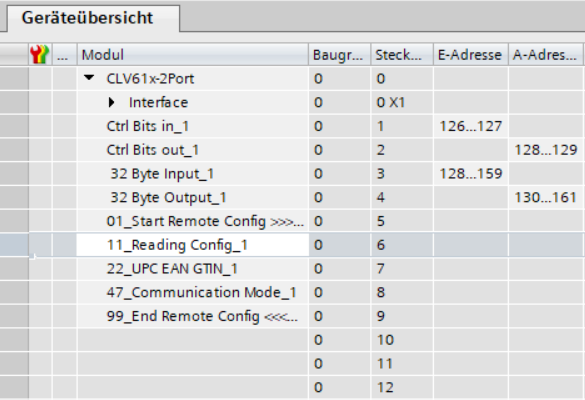
\includegraphics[width=0.6\textwidth]{Sensors/BarScan_Geräteübersicht.png}
    \caption{Barcodescanner Geräteübersicht im TIA-Portal\cite{BarScan_pic}}
    \label{BarScan_TIA}
\end{figure}

Die vom Barcodescanner belegten Ein- und Ausgangsadressen sind in der Geräteübersicht ersichtlich (siehe Abb.\ref{BarScan_TIA}). Ein TriggerBit wird verwendet um das Einlesen eines Barcodes zu starten, dabei handelt es sich um das zweite Bit des \enquote{\mbox{Ctrl Bits out\_1}} Moduls (hier: Q129.0). Bei steigender Flanke des ToggleBits wird der Laser eingeschaltet, erst bei der fallenden Flanke wird daraufhin der Code eingelesen.\\
Die eingelesenen Daten liegen ab dem ersten Input Byte (hier: ab IB128.0). Auf dem ersten Input Byte wird am vierten Bit ein ToggleBit mitgeführt. Am zweiten Byte(IB129.0) befindet sich ein Zähler, der mitzählt, wie viele Codes bereits eingelesen wurden. Das vierte Input Byte (IB131.0) gibt die Länge des eingelesenen Strings an. Ab dem sechsten Byte (IB133.0) stehen die eigentlichen Daten des Barcodes.\\
Um die Daten des Barcodes überprüfen zu können eignet sich eine wie in Abb.\ref{} abgebildete Beobachtungstabelle. Wichtig ist, dass beim Einfügen der Ein- und Ausgangsadressen das richtige Zeichenformat ausgewählt wird. Um eine Überprüfung durchzuführen lässt sich das ToggleBit zum Starten es Einlesevorgangs über Eingabe von TRUE und FALSE setzen, und daraufhin ein Code scannen. Die einzelnen Input Bytes werden daraufhin in der Tabelle angezeigt. \textbf{Foto einfügen!!}

\subsection{AS-Interface}

\subsubsection{Allgemeines}

\subsubsection{Programmierung im TIA-Portal}

\subsubsection{Verkabelung}


\subsection{Sicherheitstechnik}
\subsubsection{Grundanforderungen und Planung}
\subsubsection{Realisierung}


\newpage


\section{Resümee}


\section{Anhang}

\subsection{Abmessungen (BSVN)}


\begin{figure}[H]
    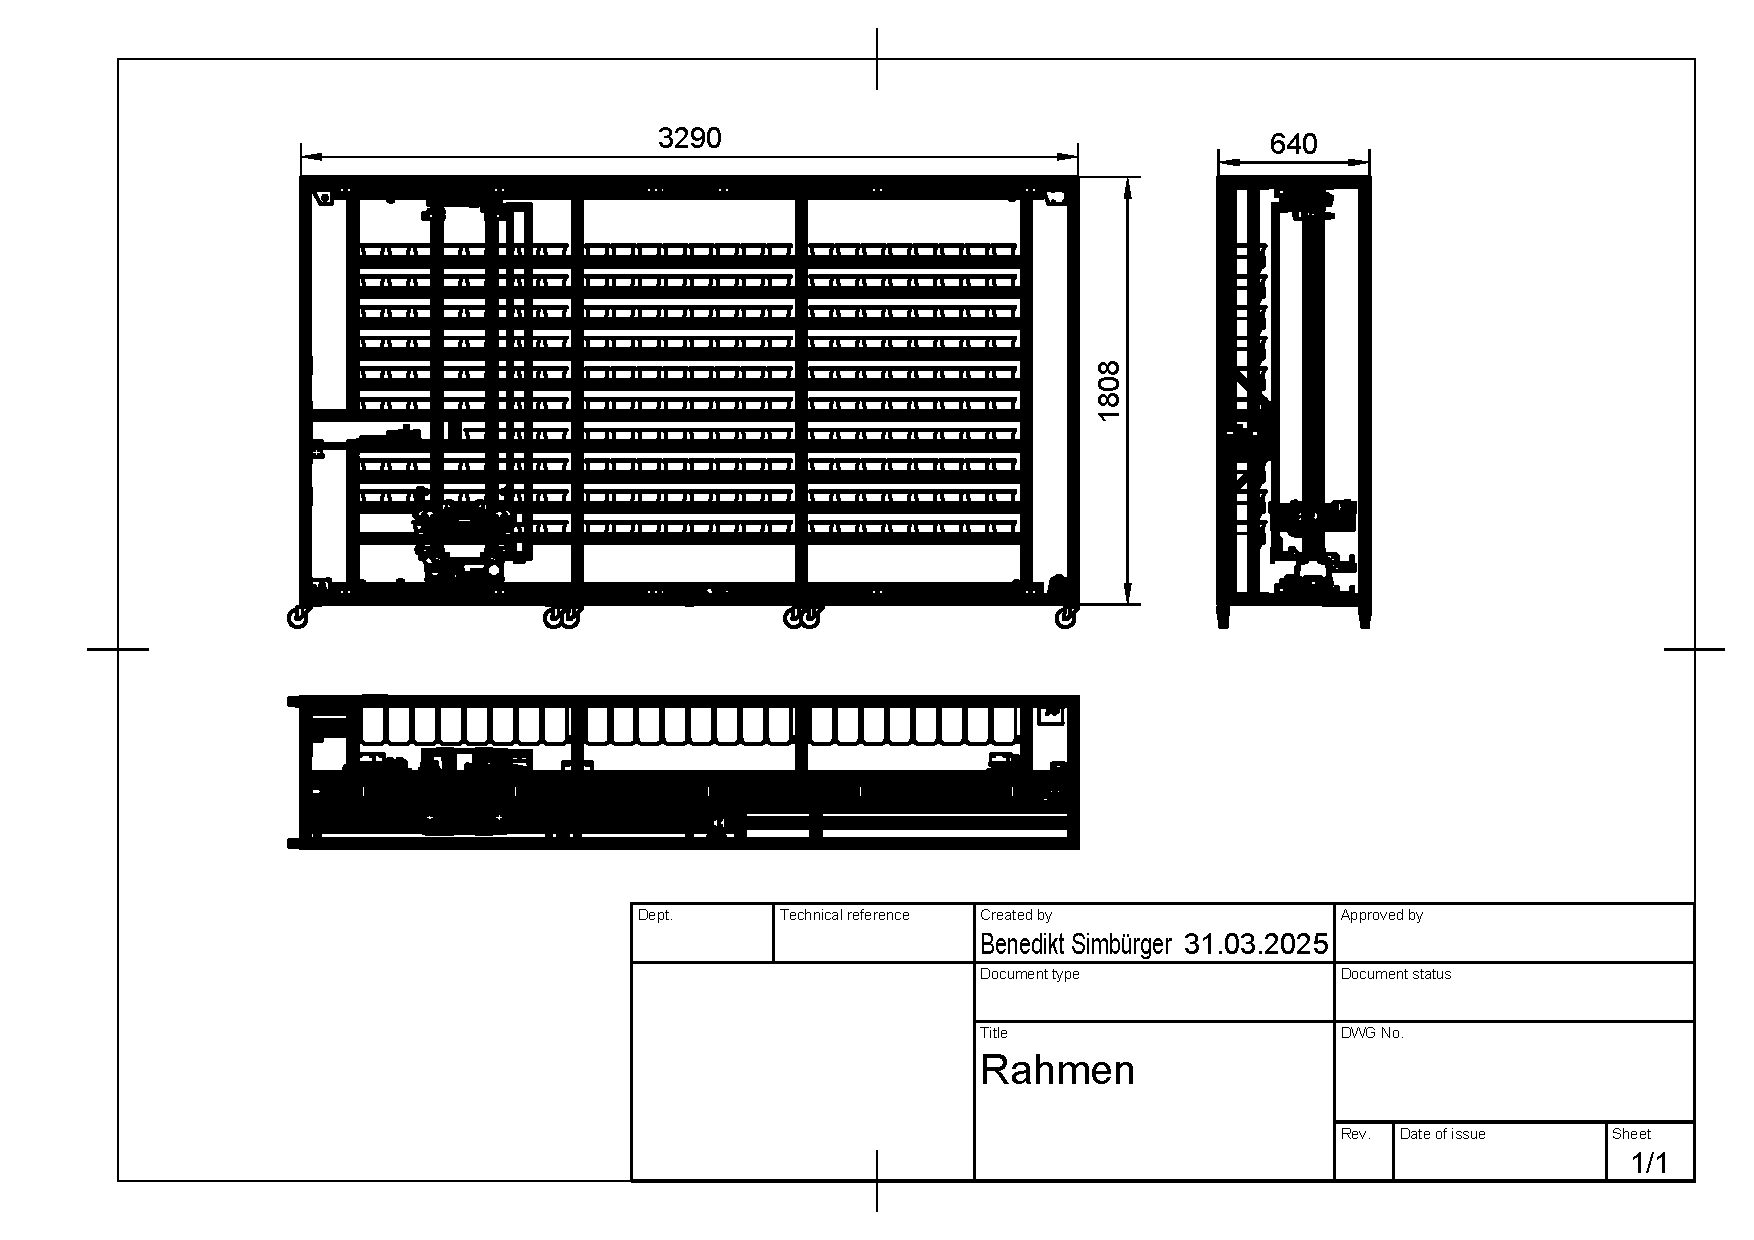
\includegraphics[width=\textwidth]{abmessungen_rahmen.pdf}
    \centering
    \caption{Abmessungen Rahmen}
\end{figure}
\begin{figure}[H]
    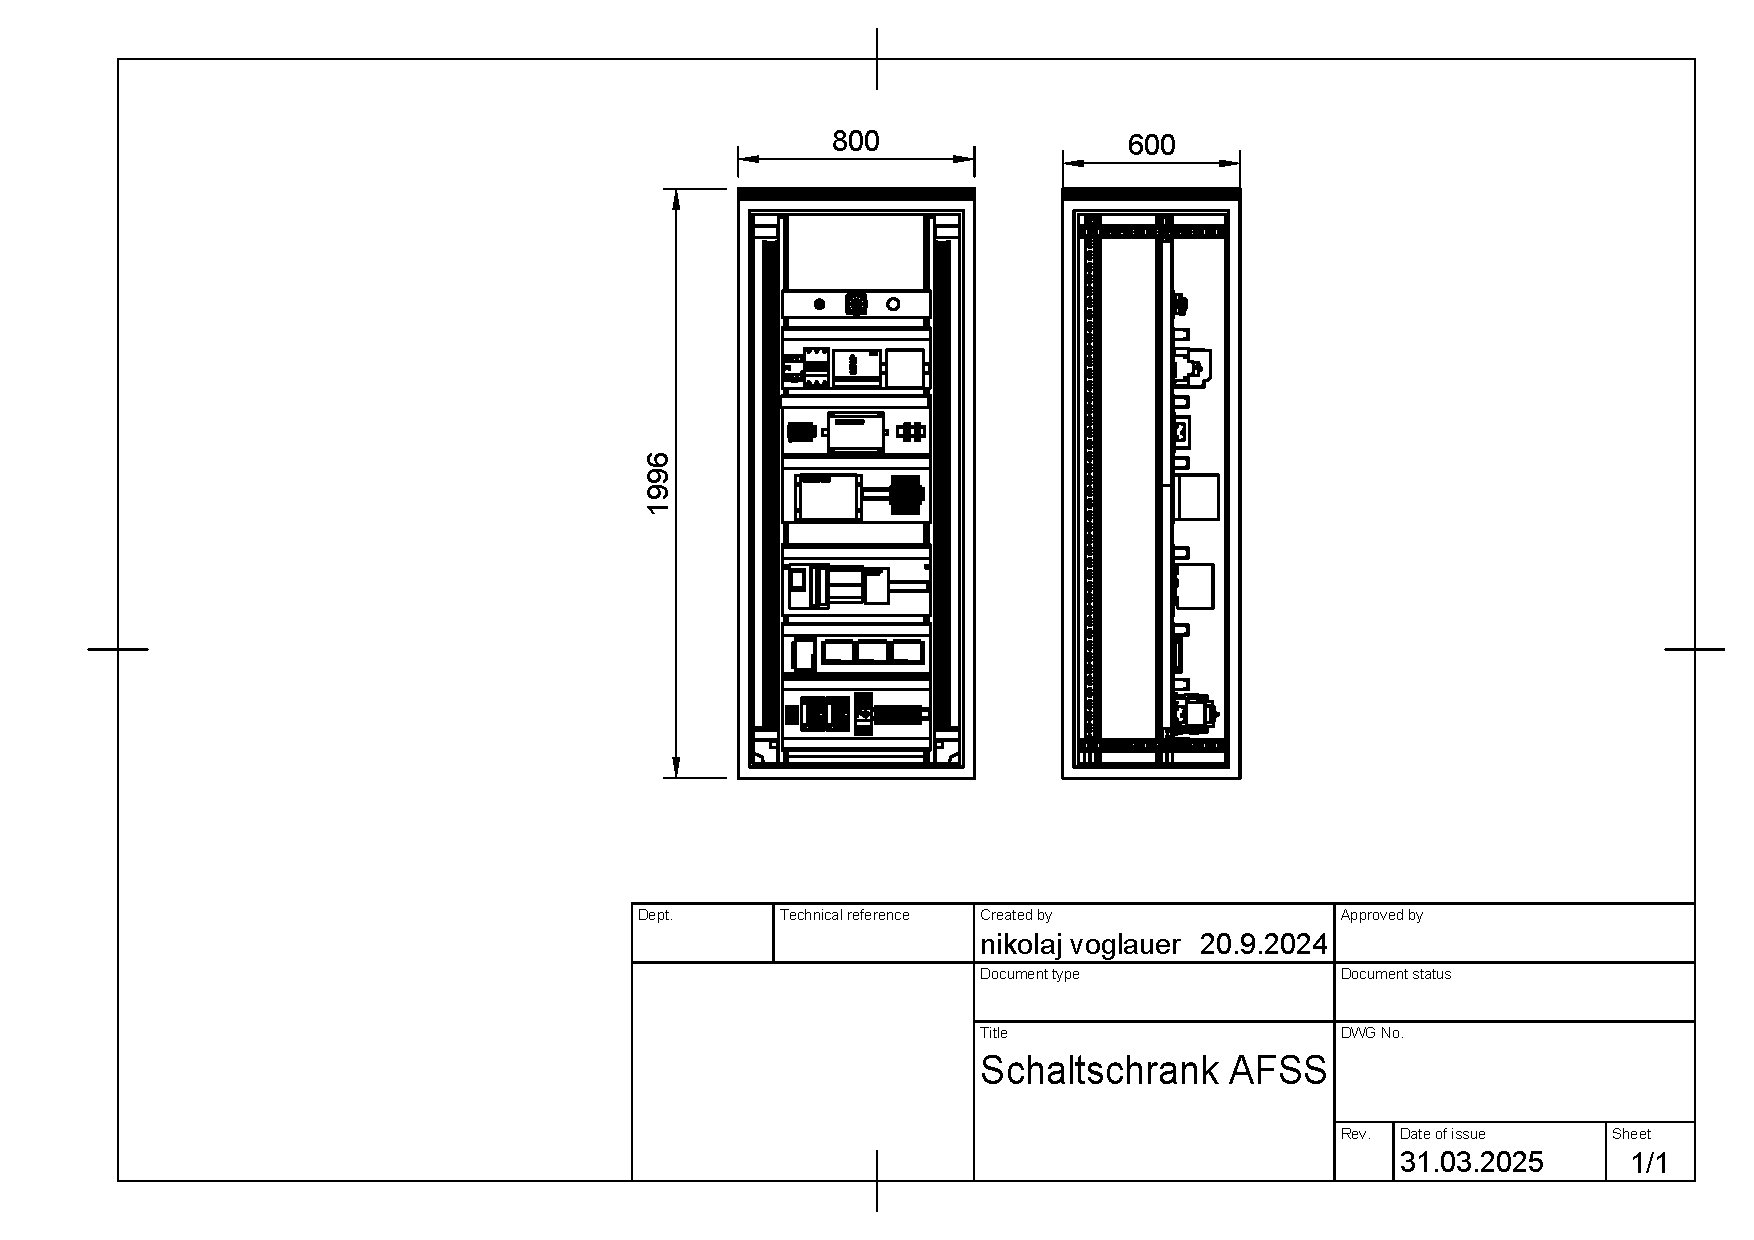
\includegraphics[width=\textwidth]{Vogis Bilder/Maximaldaten.pdf}
    \centering
    \caption{Abmessungen Rahmen}
\end{figure}

\subsection{E-Plan}

\subsection{Projektmanagement}
In diesem Kapitel wird auf das Projektmanagement des AFSS eingegangen. Dieses umfasst die zu Beginn des Projekts ausgearbeitete Aufgabenstellung und die einzelnen Arbeitspakete der jeweiligen Schülerin und Schüler. Außerdem wurde ein Produktstrukturplan angefertigt, in dem die Teilbereiche des Projekts und dessen zuständige Schülerin oder Schüler erkennbar ist. Ein weiterer Teil es Projektmanagements ist der Projektstrukturplan, welcher die unterschiedlichen Arbeitsschritte des Projekts veranschaulicht. Dieses Kapitel beinhaltet auch die in MS Project angefertigte Terminplanung.

\subsubsection{Aufgabenstellung des Gesamtprojekts}
\paragraph{Ausgangslage}\mbox{}\\
Die Werkstätte hat ein bestehendes Lager für Bauteile, die von Fachlehrern bestellt werden können. Jene Bestellungen werden dann von Schülerinnen und Schüler zusammengestellt und geliefert. Die Verwaltung dieses Lagers gestaltet sich allerdings schwierig, da Schülerinnen und Schüler beim manuellen Ein- und Auslagern z.B. den Lagerplatz vertauschen und es zu Fehlern kommt.

\paragraph{Untersuchungsanliegen der individuellen Themenstellungen}\mbox{}\\
Das Hauptanliegen dieser Diplomarbeit ist es, eine Anlage zu entwickeln, errichten und in Betrieb zu nehmen. Das bestehende System, mit manueller Handhabung, ist aufgrund des stetigen Bedienerwechsels sowie deren Ungenauigkeit, fehleranfällig. Der dadurch entstehende Mehraufwand verbraucht zusätzliche Ressourcen des Lehrpersonals. Um das Lehrpersonal sowie die Schülerinnen und Schüler zu entlasten, soll hier eine automatisierte Lösung entstehen. Es soll erwogen werden, welche Lösungen nötig sind, um ein Produkt zu planen und zu bauen, sodass dieses auch von nachfolgenden Schülerinnen und Schülern für zukünftige Anforderungen erweitert werden kann. Auch die Schnittstellen zwischen Hardware und Software, sowie die Ansteuerung der Mechanik soll in diesem Rahmen untersucht werden. Zudem soll die Sicherheit der Benutzerinnen und Benutzer immer gewährleistet sein.\\
\textbf{Simbürger Benedikt:} Programmierung des Backend und Hardwareentwicklung\\
\textbf{Sonvilla Vincent:} SPS-Programmierung und Serverkommunikation\\
\textbf{Voglauer Nikolaj:} Schaltschrankbau und Verkabelung sowie Hardwareentwicklung für Querförderer und Förderband\\
\textbf{Widmann Elena:} Auslegen elektrischen Komponenten, Ansteuerungen über Bussysteme und Sicherheitskonzeptionierung

\paragraph{Zielsetzung}\mbox{}\\
Erstellung einer Anlage, welche automatisch die gewünschte Ware mittels eines dreiachsigen Roboters, bereitstellt. Über eine Website soll eine Bestellung eingereicht werden können und der Server soll dann mit der SPS kommunizieren. Die Anlage lagert die Bestellung aus und nach Gebrauch wieder ein. Das effiziente Lagersystem soll ein hochtechnisiertes Vorzeigeprojekt der Schule werden.

\paragraph{Geplantes Ergebnis der individuellen Themenstellungen}\mbox{}\\
Die vom Benutzer gewünschten Bauteile werden aus einem Lagerplatz zu einer Kommissionier-Station gebracht und wieder zurückgestellt. Zum Herausheben der Bauteile, welche sich in Boxen befinden, ist ein vertikal montierter Portalroboter, an welchem eine Gabel montiert ist, verbaut. Ein Querförderer schiebt die angeforderten Boxen zwischen einem Förderband, welches die Boxen zum Endkunden befördert, und dem Lagersystem hin- und her. Die Bestellung ist über einen Web-Server möglich, welcher mit einer SPS kommuniziert.

\subsubsection{Produktstrukturplan}
\vspace{5mm}

\bgroup
    \centering
    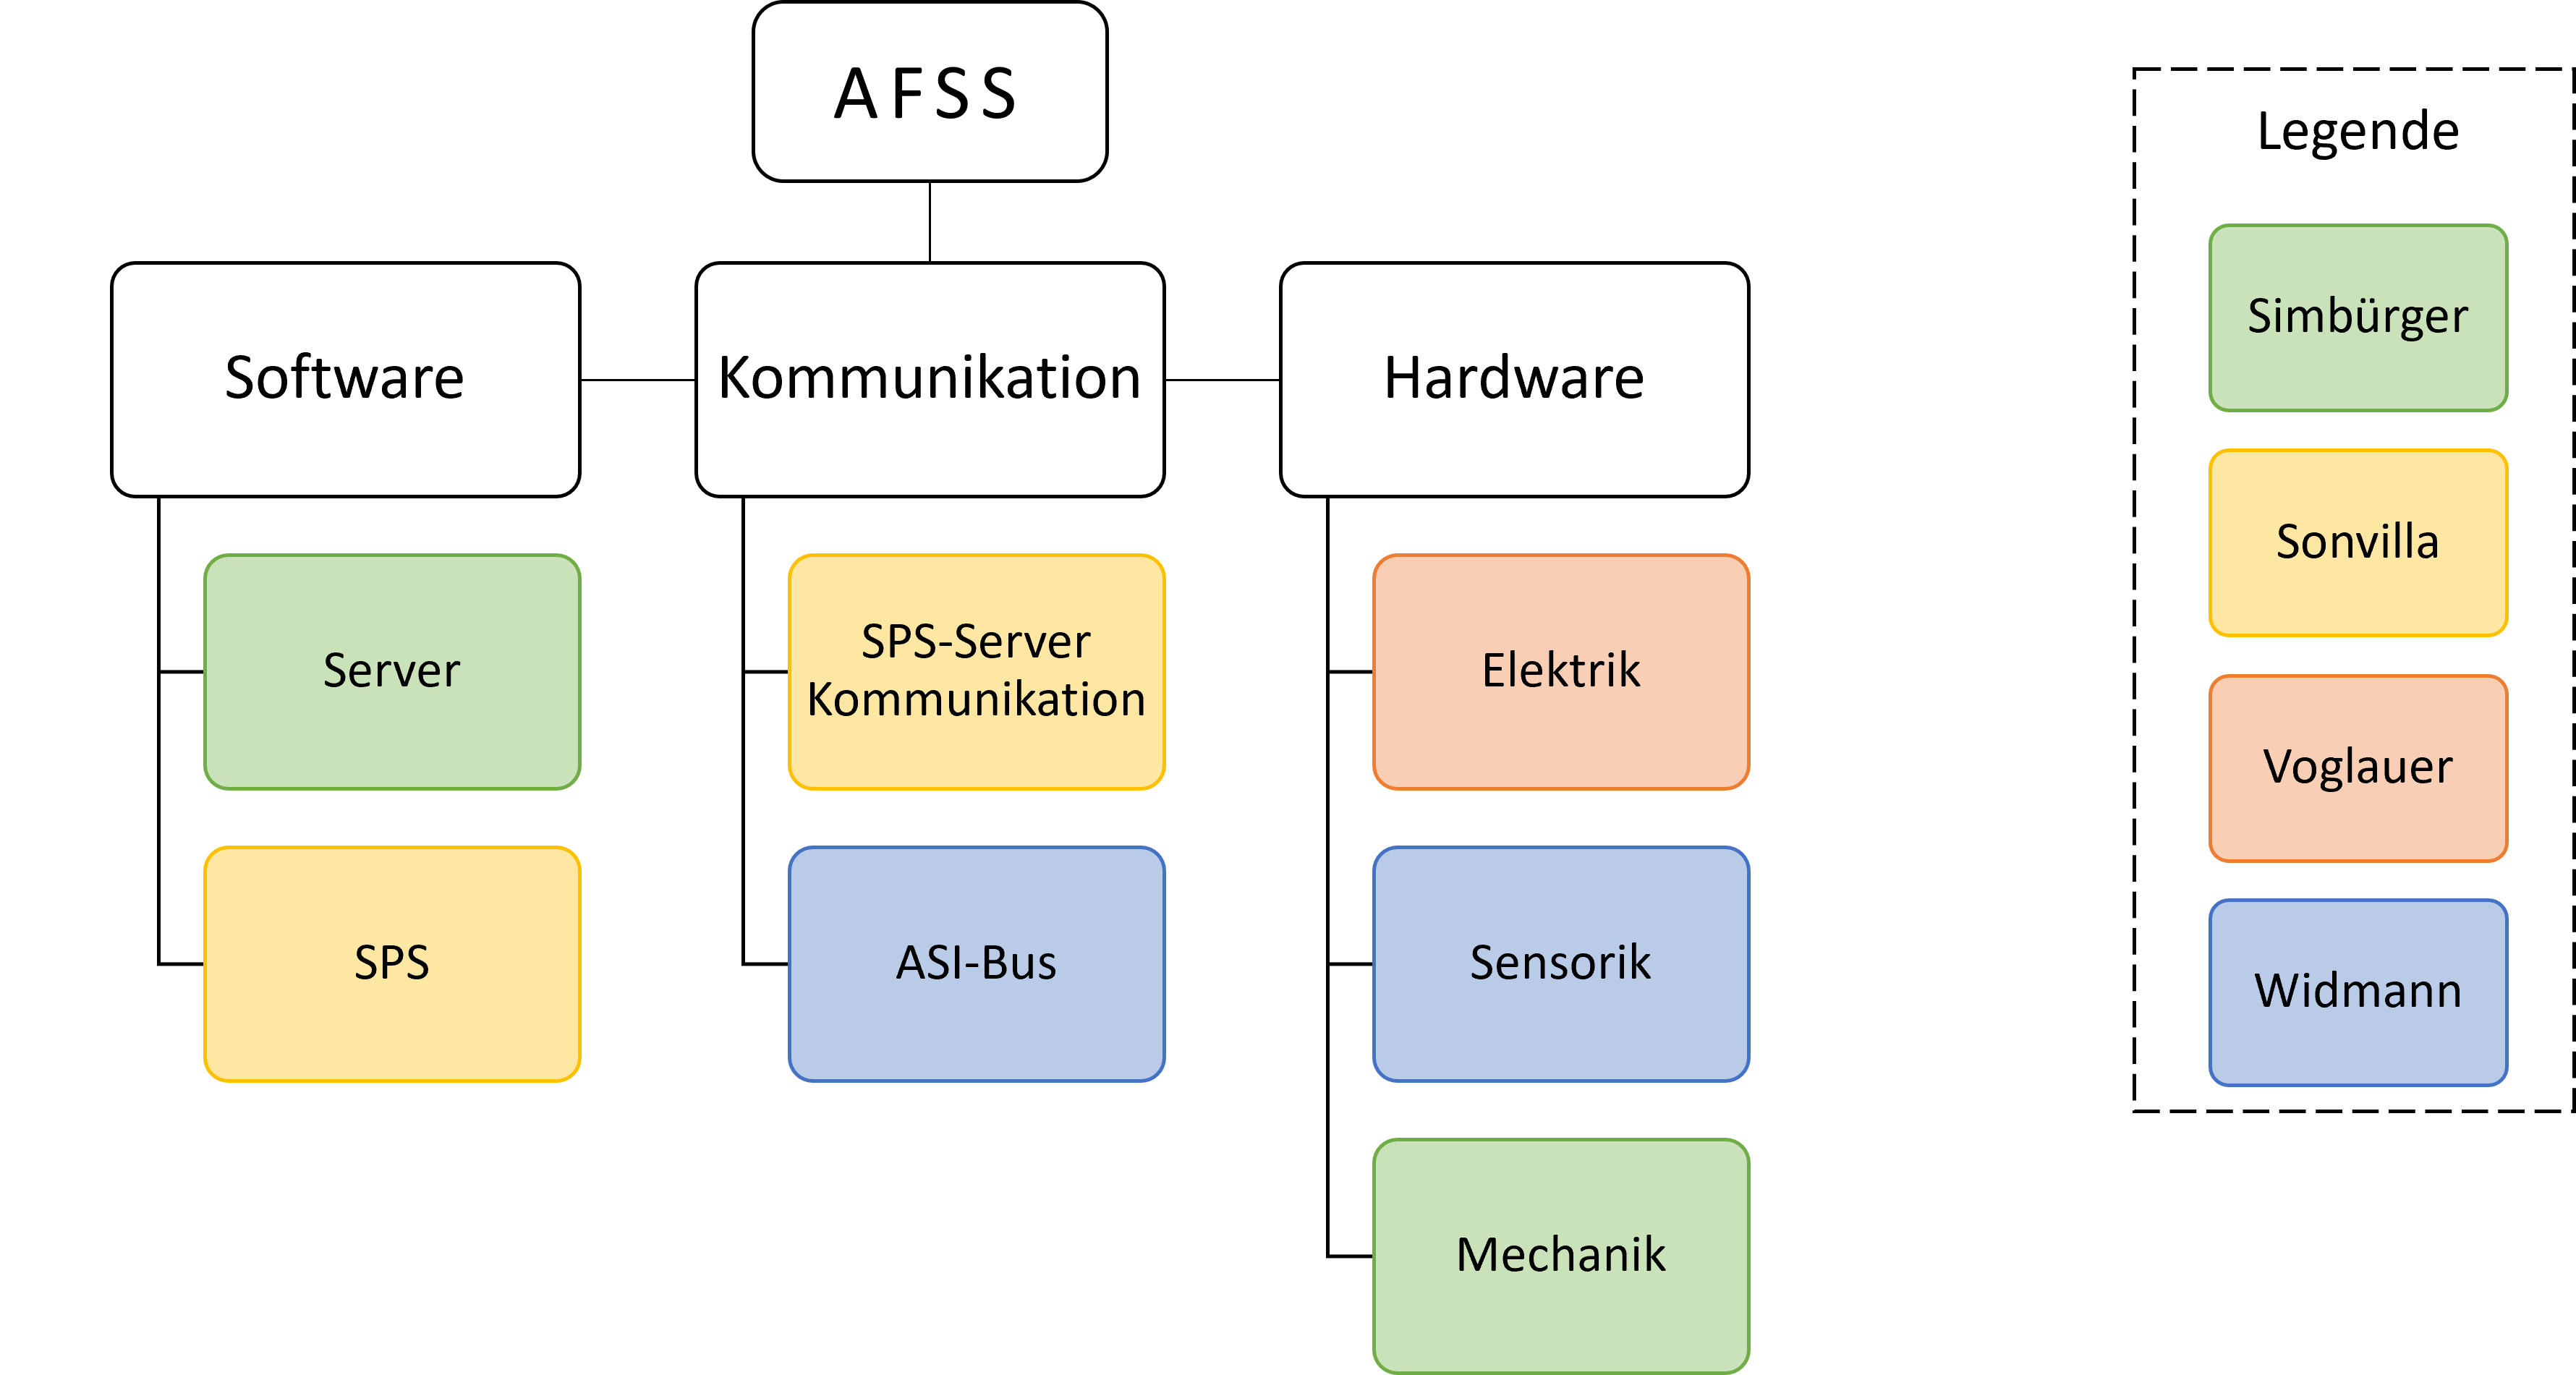
\includegraphics[width=0.9\textwidth]{WorkBreakdownStructure.png}
    \captionof{figure}{Produktstrukturplan}
\egroup

\subsubsection{Projektstrukturplan}
\vspace{5mm}

\bgroup
    \centering
    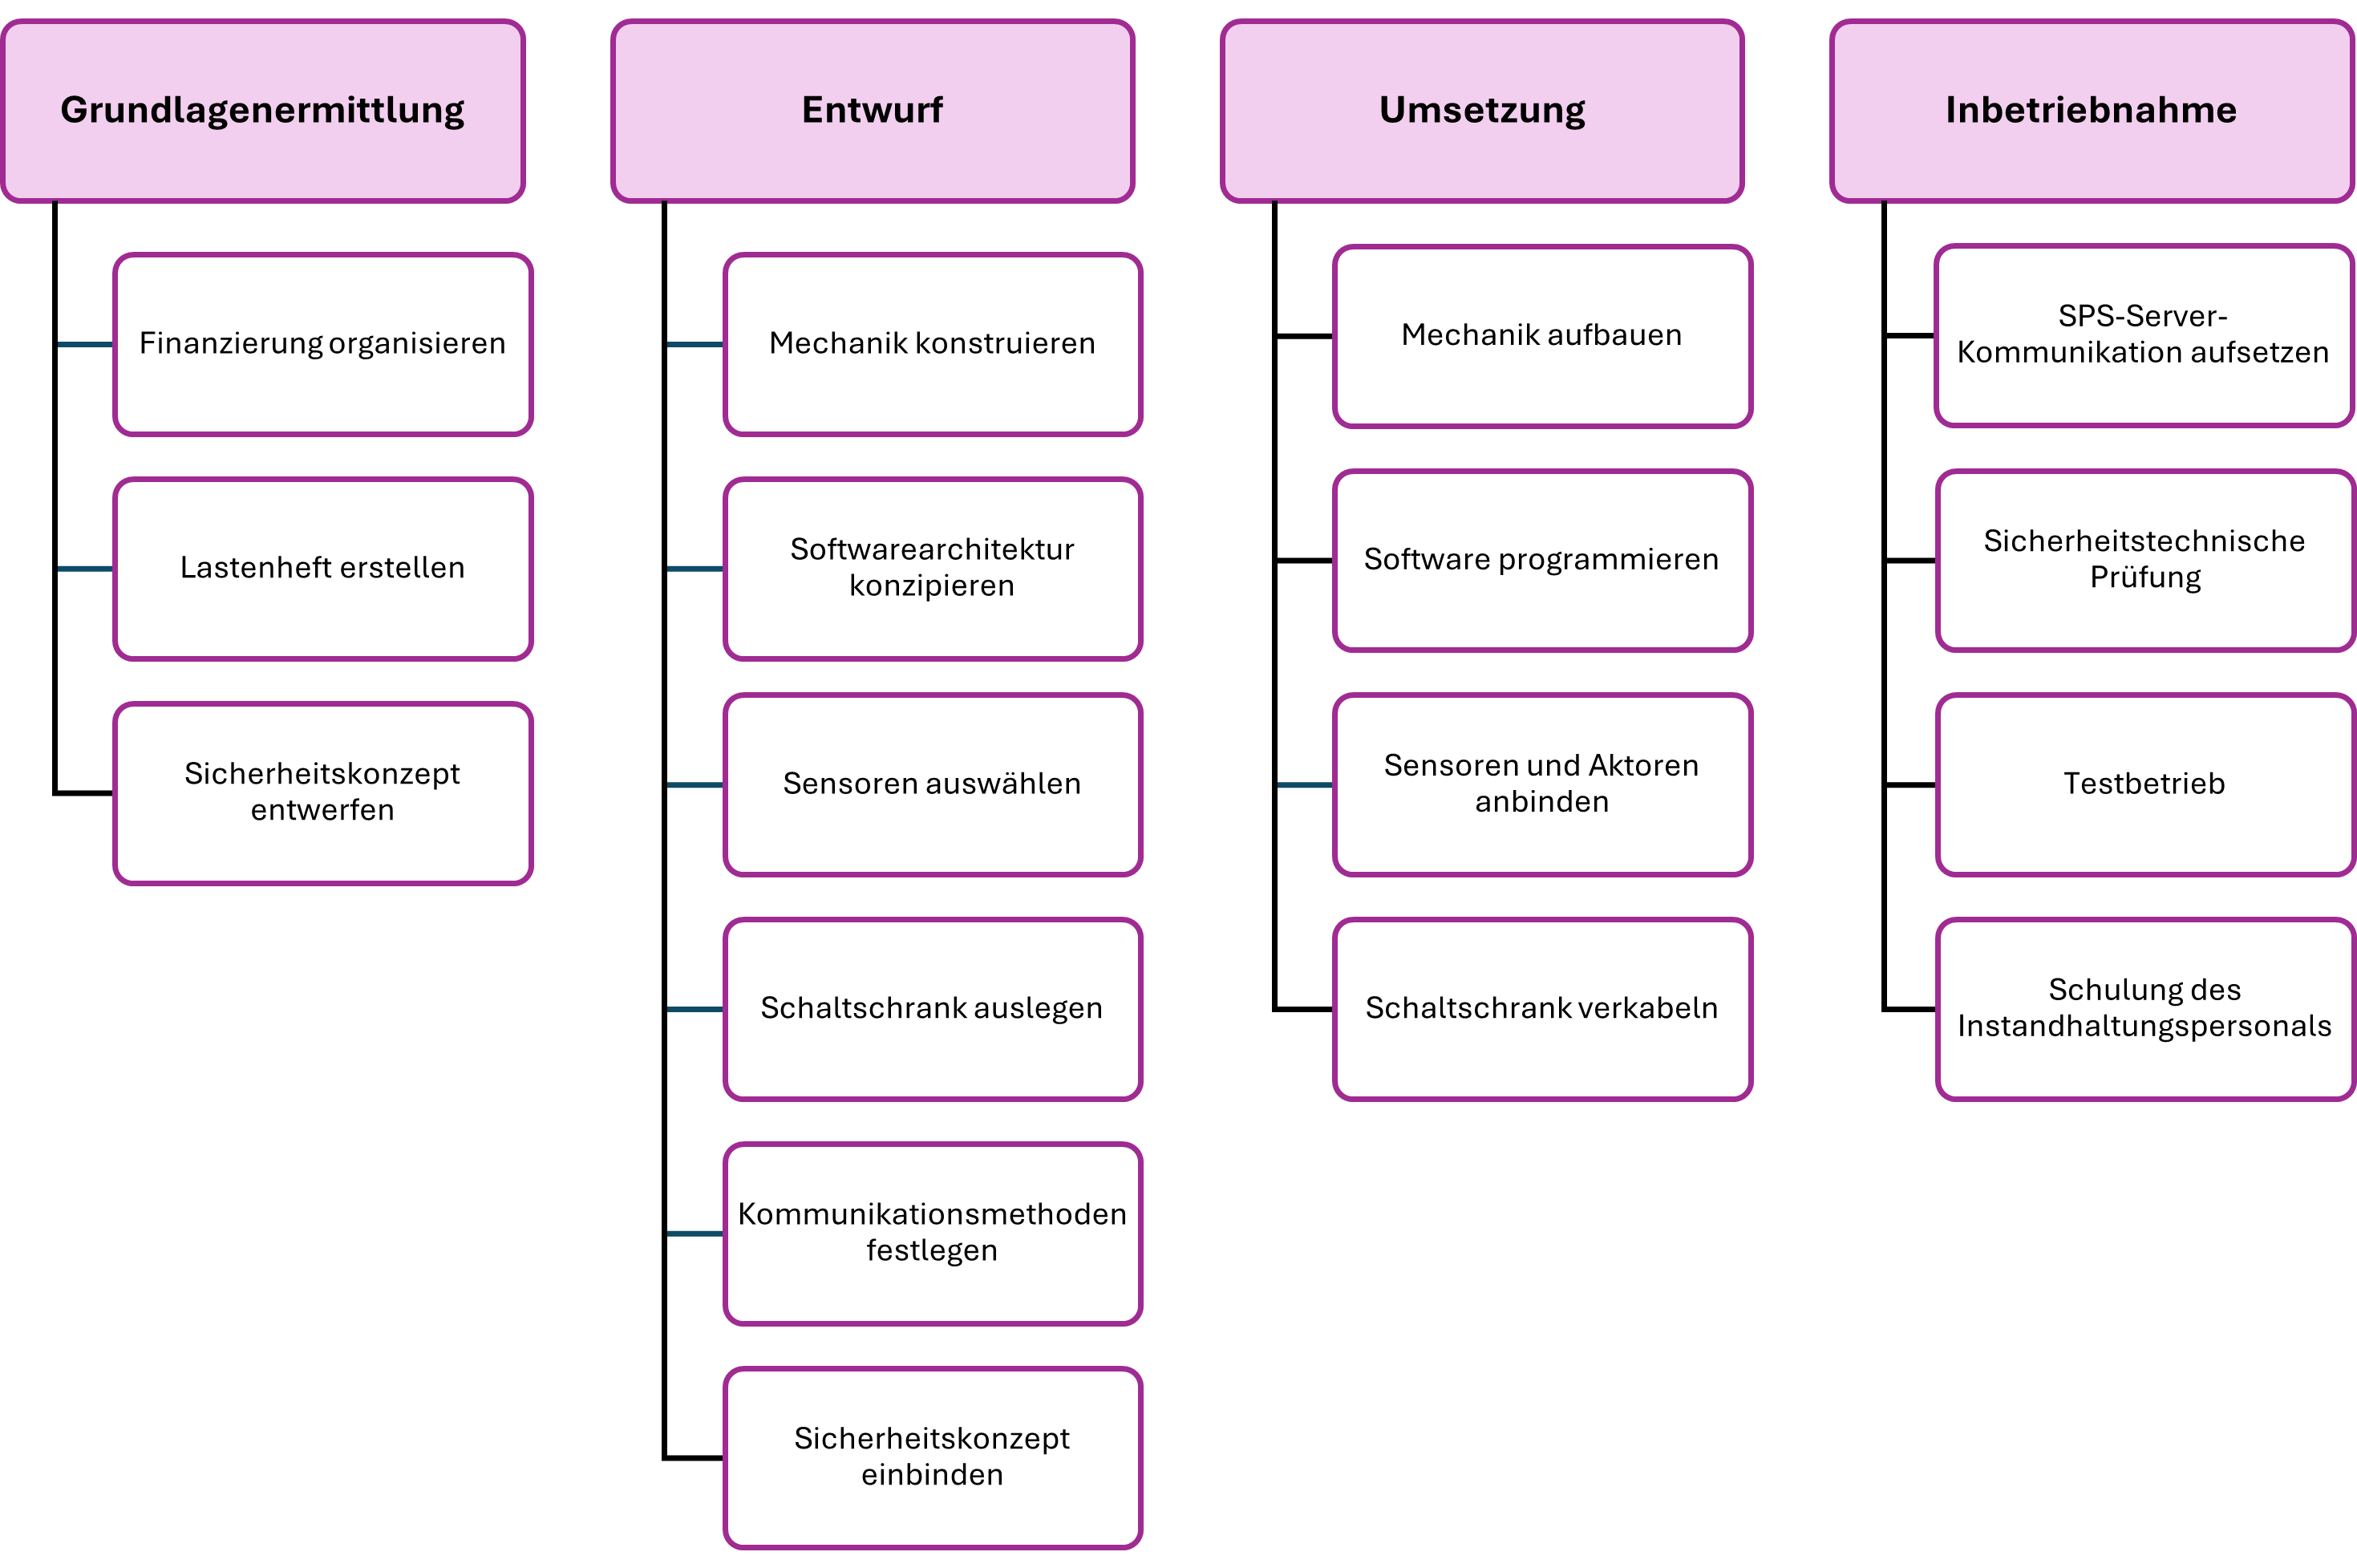
\includegraphics[width=0.9\textwidth]{ProjektStrukturPlan.png}
    \captionof{figure}{Projektstrukturplan}
\egroup

\newpage
\subsubsection{Terminplanung}
\vspace{5mm}

\bgroup
    \centering
    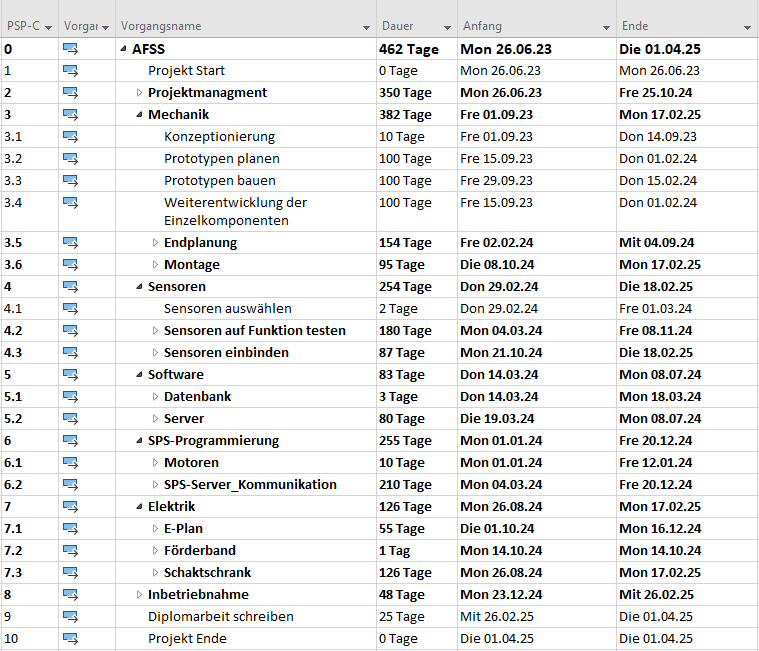
\includegraphics[width=1\textwidth]{Terminplanung.png}
    \captionof{figure}{Terminplanung in MS Project}
\egroup

\newpage

\subsubsection{Arbeitspakete}

\paragraph{Maschinenbau (Simbürger)}
\begin{itemize}
    \item Konzeptionierung des Gesamtsystem
    \item CAD - Planung
    \item Komponentenfertigung
    \item Aufbau 
\end{itemize}

\paragraph{Softwareentwicklung (Simbürger)}
\begin{itemize}
    \item Benutzeroberfläche
    \item Warehouse Management System
    \item Datenbanken
\end{itemize}

\paragraph{Elektrische Planung und Realisierung (Voglauer)}
\begin{itemize}
    \item Dokumentation vorhandener Geräte und Abmessungen dieser sowie vom Serverschrank 
    \item Zeichnen des Serverschrankes in Fusion 360
    \item Zeichnen der Module in Fusion 360
    \item Zeichnen des Schaltplanes in E-Plan 
    \item Zeichnen von Topologien und Übersichten in E-Plan 
    \item Herstellung von Modulen 
    \item Umbauten am Serverschrank
    \item Verdrahtung des Schaltschrankes
\end{itemize}

\paragraph{Sensorik (Widmann)}
\begin{itemize}
    \item Auswahl der Sensoren
    \item Referenzplatine
    \item Funktionsprüfungen und Messungen
    \item AS-Interface
\end{itemize}

\paragraph{Sicherheitstechnik (Widmann)}
\begin{itemize}
    \item Entwicklung eines Sicherheitskonzepts
    \item Realisierung
\end{itemize}




\newpage

\subsection{Inbetriebnahme}

\subsubsection{Server}

Der Server kann auf zwei unterschiedliche Arten in Betrieb genommen werden.  

\paragraph{Entwicklungsmodus} \mbox{}\\ 

Um beim Entwickeln einen angenehmeren Prozessablauf zu ermöglichen, kann der Server klassisch durch Starten des Programms mit Python ausgeführt werden.  
Hierzu sollte zuerst eine neue virtuelle Python-Umgebung aufgesetzt und die Pakete aus der Datei \texttt{requirements.txt} geladen werden. Alternativ kann die beim Entwickeln verwendete virtuelle Umgebung im \texttt{.conda}-Ordner genutzt werden.  

Nach Aktivierung der virtuellen Umgebung kann der Server durch Ausführen des Befehls  
\begin{verbatim}
python __init__.py
\end{verbatim}  
im Ordner \texttt{Prototyp\_2} gestartet werden.  
Im Terminal erscheinen dann die Logs des Einschaltvorgangs, einschließlich der IP-Adresse und des Ports, auf dem der Server läuft.  
Jedoch muss die Datenbank, um eine Verbindung herstellen zu können, separat gestartet werden.  
Die Verbindungsdaten für die Datenbank sowie viele weitere Konfigurationen können in der Datei \texttt{config.py} angepasst werden.  

\paragraph{Docker} \mbox{}\\

Für einen Serverbetrieb in einer Produktionsumgebung besteht die Möglichkeit, den Server über einen Docker-Container zu starten.  
Nach der Installation von Docker muss im übergeordneten Ordner von \texttt{Prototyp\_2}, in dem sich die Datei \texttt{docker-compose.yml} befindet, folgender Befehl ausgeführt werden:  

\begin{verbatim}
docker compose -f 'docker-compose.yml' up -d --build
\end{verbatim}  

Dadurch wird ein Container erstellt, der anschließend entweder in Docker-Desktop oder über die Kommandozeile gestartet werden kann.  
Da die Datenbank beim ersten Start auf einer Fremdmaschine noch kein Setup durchlaufen hat, ist es ratsam, sie mit einer Sicherungsdatei aus dem Ordner \texttt{DB\_export} aufzusetzen.  
Danach bleiben die Daten auch nach dem Abschalten des Containers erhalten.  

Jedoch ist es nach der Implementierung des Rust-Pakets noch nicht möglich, die benötigten Bibliotheken zu installieren, da diese nicht im \texttt{docker-compose.yml} enthalten sind. 



\subsubsection{Schaltschrank}
    Der Schaltschrank ist möglichst benutzerfreundlich. Zum Inbetriebnehmen ist eine Starkstromleitung an den dafür vorgesehenen Klemmen zu legen. Ist dies gegeben muss der Dreh-Trennschalter nun geschalten werden und die Anlage wird versorgt. Um die Anlage freizugeben ist der Schlüsselschalter zu betätigen.\\
    Beim Inbetriebnehmen ist zu beachten, dass keine Warnleuchten an den elektirschen Komponenten leuchten und es ist auf untypische Geräusche oder Gerüche zu achten. Bei etwaigen Auffälligkeiten ist die Anlage sofort mitels Trennschalter freizuschalten und daraufhin soll die Quelle der Auffälligkeit gefunden werden und, wenn vorhanden, der Fehler behoben werden.\\
    Zur Inbetriebnahme gehört auch, dass der FI und der Leitungsschutzschalter einmal getestet beziehungsweise geschalten werden um die Funktion zu testen.\\
\color{blue}
Nachdem typische Projekte aus mehreren Komponenten bestehen, ist es oft nicht trivial die einzelnen Komponenten korrekt zu konfigurieren und das Gesamtsystem in Betrieb zu nehmen. In diesem Kapitel soll eine vollständige, präzise und trotzdem möglichst kompak-te Anleitung zur Inbetriebnahme des Systems dargelegt werden. Die Schritte sollen in dem Detailgrad beschrieben werden, dass ein durchschnittlicher Schüler des vierten Jahrganges das Projekt in Betrieb nehmen kann. Exemplarisch sollten Punkte wie die folgenden be-handelt werden – die Aufzählung ist nicht vollständig):
\begin{itemize}
    \item Treiberinstallationen und Systemkonfigurationen
    \item Zu empfehlen wäre bei Server-Installationen ein Setup-Script, welches auf einem vordefinierten Docker-container aufbaut.
    \item Welche Schritte sind notwendig, um das Projekt mit dem vorhandenen Code / Schaltplänen (auf GIT, CD, Netzlaufwerk, etc.) in Betrieb zu nehmen.
    \item Bei Schaltungen mit mehreren Platinen muss beschrieben werden, wie diese mit-einander verbunden werden müssen.
\end{itemize}
\color{black}

\newpage
\subsection{Kostenaufstellung BSNV}
\textcolor{blue}{Für die Kalkulation im Gesamtprojekt sind folgende Kosten zu erfassen: \\
•	Kosten für Material (Hard- und Software)\\
•	externe Kosten (z.B.: Zukauf von Sensoren, Funkmodule, spezielle Entwicklungsum-gebungen, etc.) 
}
\begin{figure}[h]
    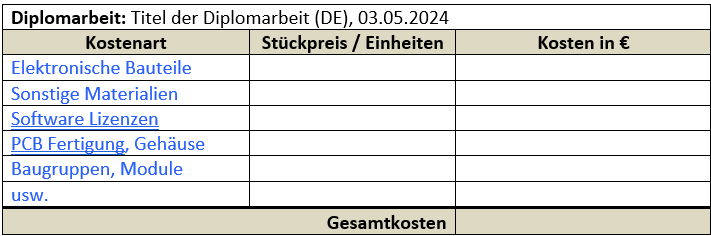
\includegraphics[width=0.8\textwidth]{Kostenaufstellung.png}
    \centering
    \caption{Kostenaufstellung}
\end{figure}


\newpage
\subsubsection{Elektrische Komponenten (Voglauer)}
Da die Käufe der Komponenten, von der Schule oder von den Sponsoren, überwiegend vor langer Zeit getätigt. Daher sind spezifische Kaufdaten nicht bekannt, die folgenden Daten schätzen somit den aktuellen Preis der Komponenten ab.\\ 
\paragraph{Kapital von der Schule}
\begin{longtable}{|p{7cm}|r|r|}
    \hline
    \textbf{Komponente} & \textbf{Stückzahl} & \textbf{Preis} \\
    \hline
    \endfirsthead

    \hline
    \textbf{Komponente} & \textbf{Stückzahl} & \textbf{Preis} \\
    \hline
    \endhead

    \hline
    \endfoot

    \hline
    \endlastfoot
    Trennschalter & 1 & € 143,00 \\
    Schlüsselschalter & 1 & € 4,99 \\
    Not-Aus-Schalter & 4 & € 12,65 \\
    Motorschutzschalter & 1 & € 55,45 \\
    Fehlerstromschutzschalter Typ A & 1 & € 221,20 \\
    Leitungsschutzschalter C13 & 1 & € 25,00 \\
    3RK2200-0CE02-0AA2 & 7 & € 146,01 \\
    6ES7155-6AU01-0CN0 & 1 & € 300,00 \\
    6ES7193-6AR00-0AA0 & 1 & € 106,67 \\
    3RK7137-6SA00-0BC1 & 1 & € 673,04 \\
    6ES7193-6BP20-0DC0 & 1 & € 70,00 \\
    Asynchronmotor & 1 & € 200,00 \\
    CL57T(V4.0) & 4 & € 36,39 \\
    TB6560 & 3 & € 17,99 \\
    23E1K-20 & 4 & € 38,77 \\
    17HS4417P1-X4 & 3 & € 8,99 \\
    \textbf{Summe} & & € 3251,00\\
    \hline
    \hline
\end{longtable}
\paragraph{Gesponsort von der KNAPP AG}
\begin{longtable}{|p{7cm}|r|r|}
    \hline
    \textbf{Komponente} & \textbf{Stückzahl} & \textbf{Preis} \\
    \hline
    \endfirsthead

    \hline
    \textbf{Komponente} & \textbf{Stückzahl} & \textbf{Preis} \\
    \hline
    \endhead

    \hline
    \endfoot

    \hline
    \endlastfoot
    \hline
    \hline
    TSX-SUP-A054 & 1 & € 250,00 \\
    6EP1436-3BA00-8AA0 & 1 & € 350,00 \\
    DP500IP/3-24 & 1 & € 301,68 \\
    DRT-240-24 & 1 & € 97,46 \\
    6ES7515-2AN03-0AB0 & 1 & € 3.195,40 \\
    6ES7521-1BL00-0AB0 & 1 & € 332,10 \\
    6ES7553-1AA00-0AB0 & 2 & € 825,86 \\
    6ES7522-1BL01-0AB0 & 1 & € 560,49 \\
    \textbf{Summe} & & € 5.912,99\\
\end{longtable}
\paragraph{Gesponsort von der Weidmüller GmbH}
\begin{longtable}{|p{7cm}|r|r|}
    \hline
    \textbf{Komponente} & \textbf{Stückzahl} & \textbf{Preis} \\
    \hline
    \endfirsthead

    \hline
    \textbf{Komponente} & \textbf{Stückzahl} & \textbf{Preis} \\
    \hline
    \endhead

    \hline
    \endfoot

    \hline
    \endlastfoot
    \hline
    \hline
    2081870000 & 2 & € 8,41 \\
    IE-FC-SET-SPDEK001-KY-P & 1 & € 144,93 \\
    2080600000 & 4 & € 37,26 \\
    2080480000 & 2 & € 37,18 \\
    AL2C 2.5 & 100 & € 0,64 \\
    \textbf{Summe} & & € 449,15\\
\end{longtable}
\paragraph{Gesponsort von der Firma Lapp}
\begin{longtable}{|p{7cm}|r|r|}
    \hline
    \textbf{Komponente} & \textbf{Stückzahl} & \textbf{Preis} \\
    \hline
    \endfirsthead

    \hline
    \textbf{Komponente} & \textbf{Stückzahl} & \textbf{Preis} \\
    \hline
    \endhead

    \hline
    \endfoot

    \hline
    \endlastfoot
    \hline
    \hline
    ÖLFLEX CLASSIC FD 810 CY 5x0.5 & 30m & € 117,63 \\
    ÖLFLEX CLASSIC FD 810 CY 5x0.75 & 40m & € 174,41 \\
    ÖLFLEX CHAIN 809 CY 7x0.5 & 40m & € 150,95 \\
    H05V-K 1x0.75 & 100m & € 18,86 \\
    H05V-K 1x0.75 & 100m & € 18,86 \\
    H05V-K 1x0.75 & 100m & € 18,86 \\
    \textbf{Summe} & & € 496,57\\
\end{longtable}

\paragraph{Gesamtwert der elektrischen Komponenten}\mbox{}\\
    Alle Komponenten gemeinsam verfügen über einen Geschätzten Wert von 10 109,71 €.
\newpage
<<<<<<< HEAD

\subsubsection{Igus}
\begin{table}[H]
    \begin{tabular}{llllll}
    Name                & Artikelnummer          & Menge & pro Stück {[}€{]} & Preis {[}€{]} \\ \hline
    Schlepkette X       & E2i.26.057.048.0       & 1             & 72.72                   & 72.72         \\
    Schlepkette Y       & E2i.26.038.048.0       & 1             & 49.74                   & 49.74         \\
    Gewindespindel      & DST-LS-10X12-R-ES      & 2 x 350mm              & 35.15                   & 70.3          \\
    Gewindemutter       & DST-JFRM-252525DS10X12 & 2             & 26.33                   & 52.66         \\
    Führungsschiene     & TS-01-20               & 2 x 350mm              & 16.685                  & 33.37         \\
    Führungswagen       & TW-01-20               & 2             & 35.1                    & 70.2          \\ \hline
    Gesamt              &                        &               &                         & 348.99       
    \end{tabular}
\end{table}

\subsubsection{Mädler}
\begin{table}[H]
    \begin{tabular}{lllll}
    Name                           & Artikelnummer & Menge & pro Stück {[}€{]} & Preis {[}€{]}  \\ \hline
    Zahnscheibe AT5x16 20 Zähne    & 16632000      & 2     & 7.58            & 15.16  \\
    Zahnscheibe AT5x16    27 Zähne & 16632700      & 2     & 8.7             & 17.4   \\
    Zahnscheibe AT5x16  36 Zähne   & 16633600      & 2     & 12.58           & 25.16  \\
    Zahnriemen AT5x16              & 16670000      & 21    & 16.44           & 345.24 \\ \hline
    Gesamt                         &               &       &                 & 402.96
    \end{tabular}
\end{table}

=======
<<<<<<< HEAD
\subsection{Besprechungsprotokolle}
=======
=======
>>>>>>> dceed3876735e862bab10feb1fae81db6179fa41
>>>>>>> bba1d72b5ad5c3f3b3e1e80ced846a189e1d487f
\subsection{Besprechungsprotokolle (SV)}
%include pdf file as image, on howl page with label
\begin{figure}[H]
    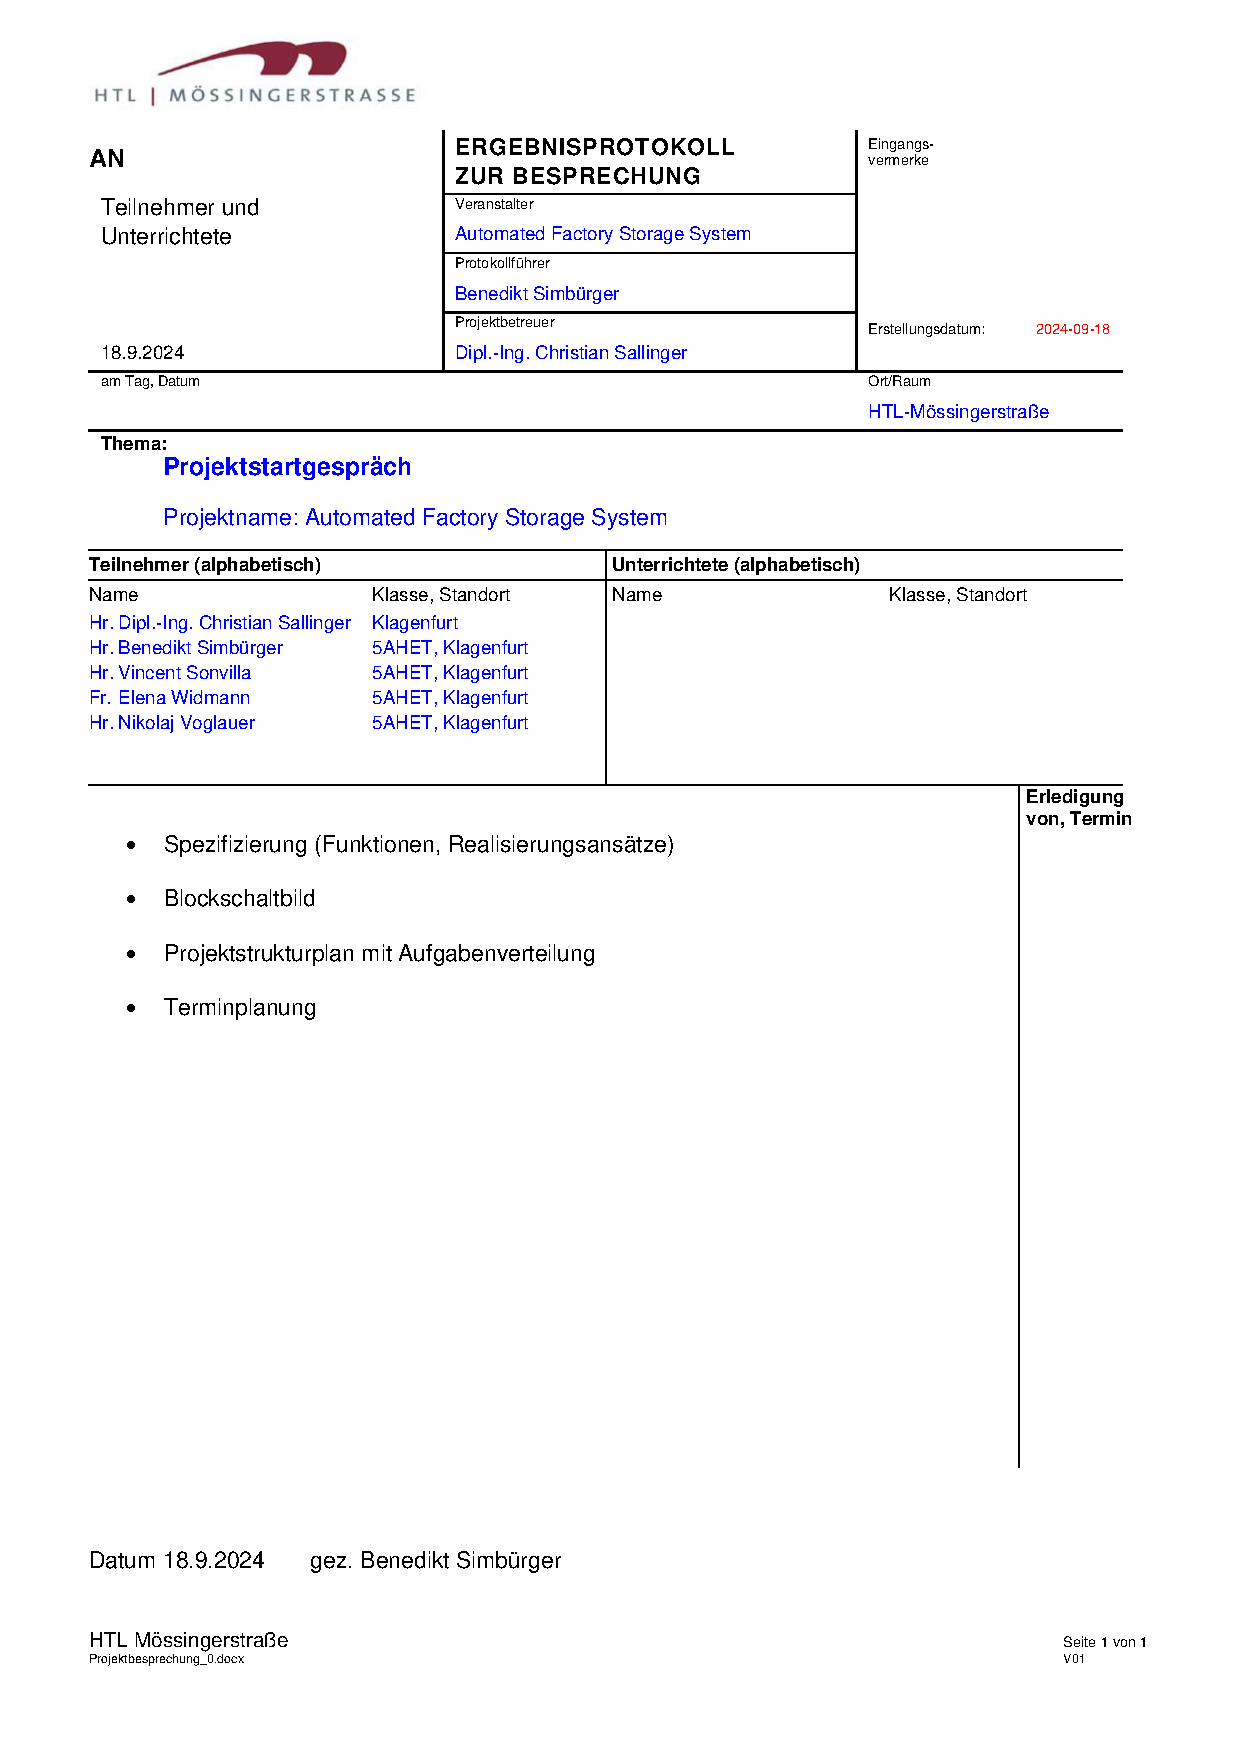
\includegraphics[width=0.9\textwidth]{../Protokolls/Projektbesprechung_0.pdf}
    \centering
    \caption{Besprechungsprotokoll 10.12.2024}
\end{figure}

\begin{figure}[H]
    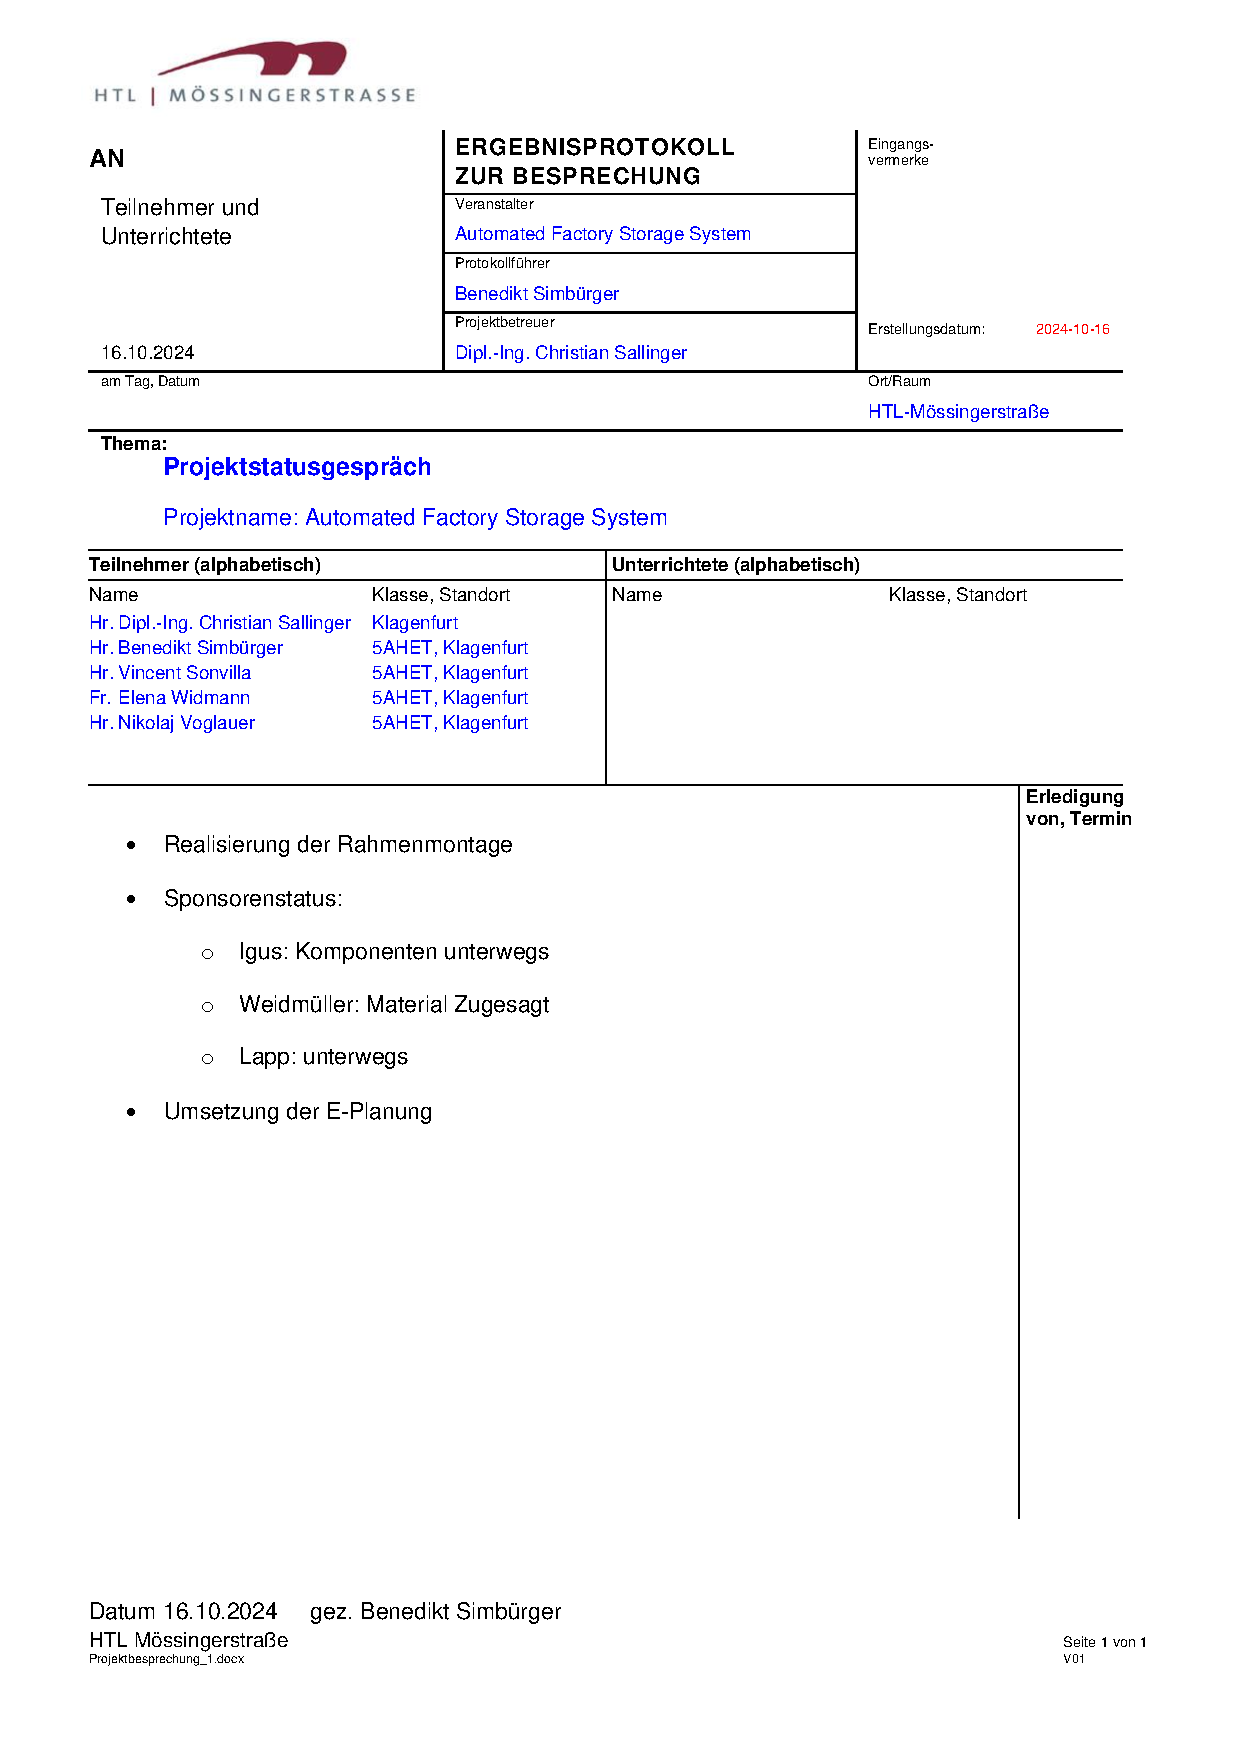
\includegraphics[width=0.9\textwidth]{../Protokolls/Projektbesprechung_1.pdf}
    \centering
    \caption{Besprechungsprotokoll 16.10.2024}
\end{figure}

\begin{figure}[H]
    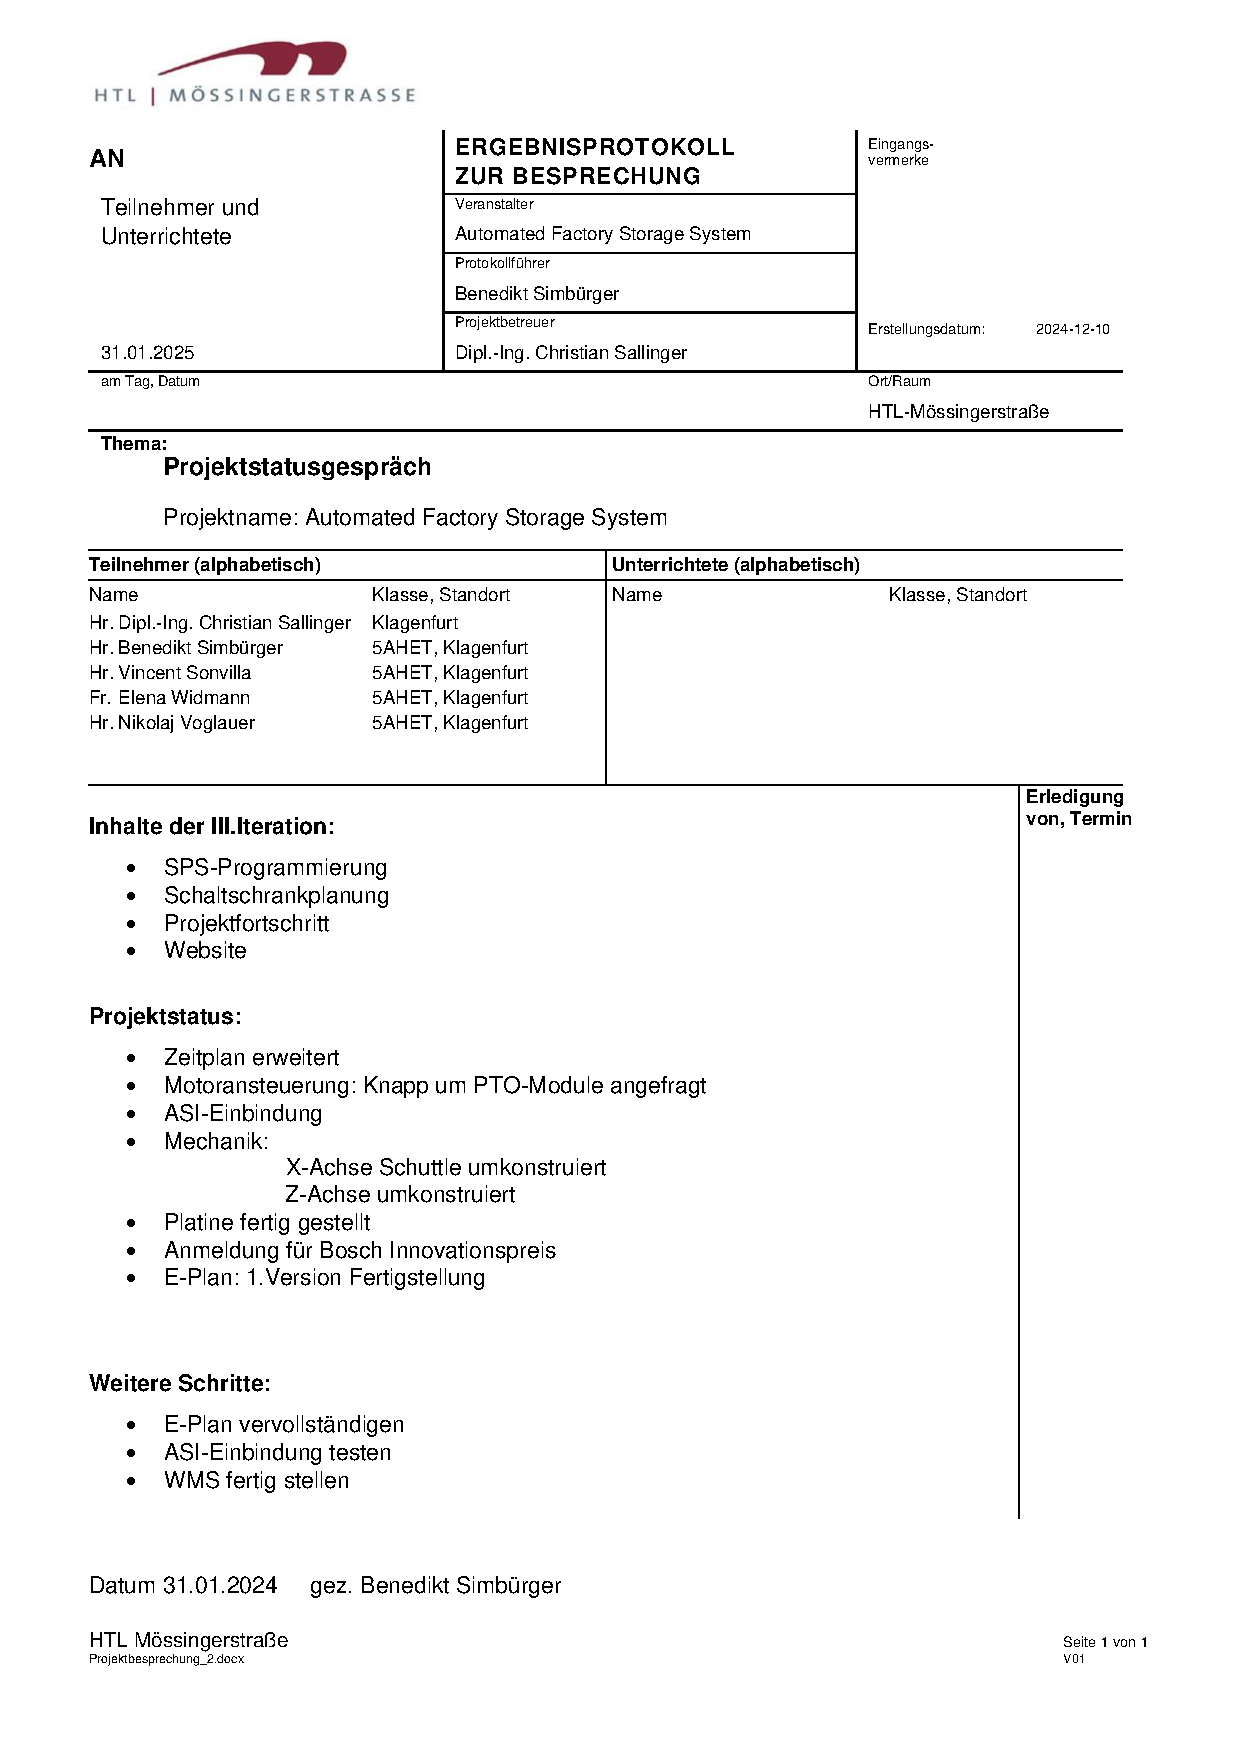
\includegraphics[width=0.9\textwidth]{../Protokolls/Projektbesprechung_2.pdf}
    \centering
    \caption{Besprechungsprotokoll 10.12.2024}
\end{figure}

\begin{figure}[H]
    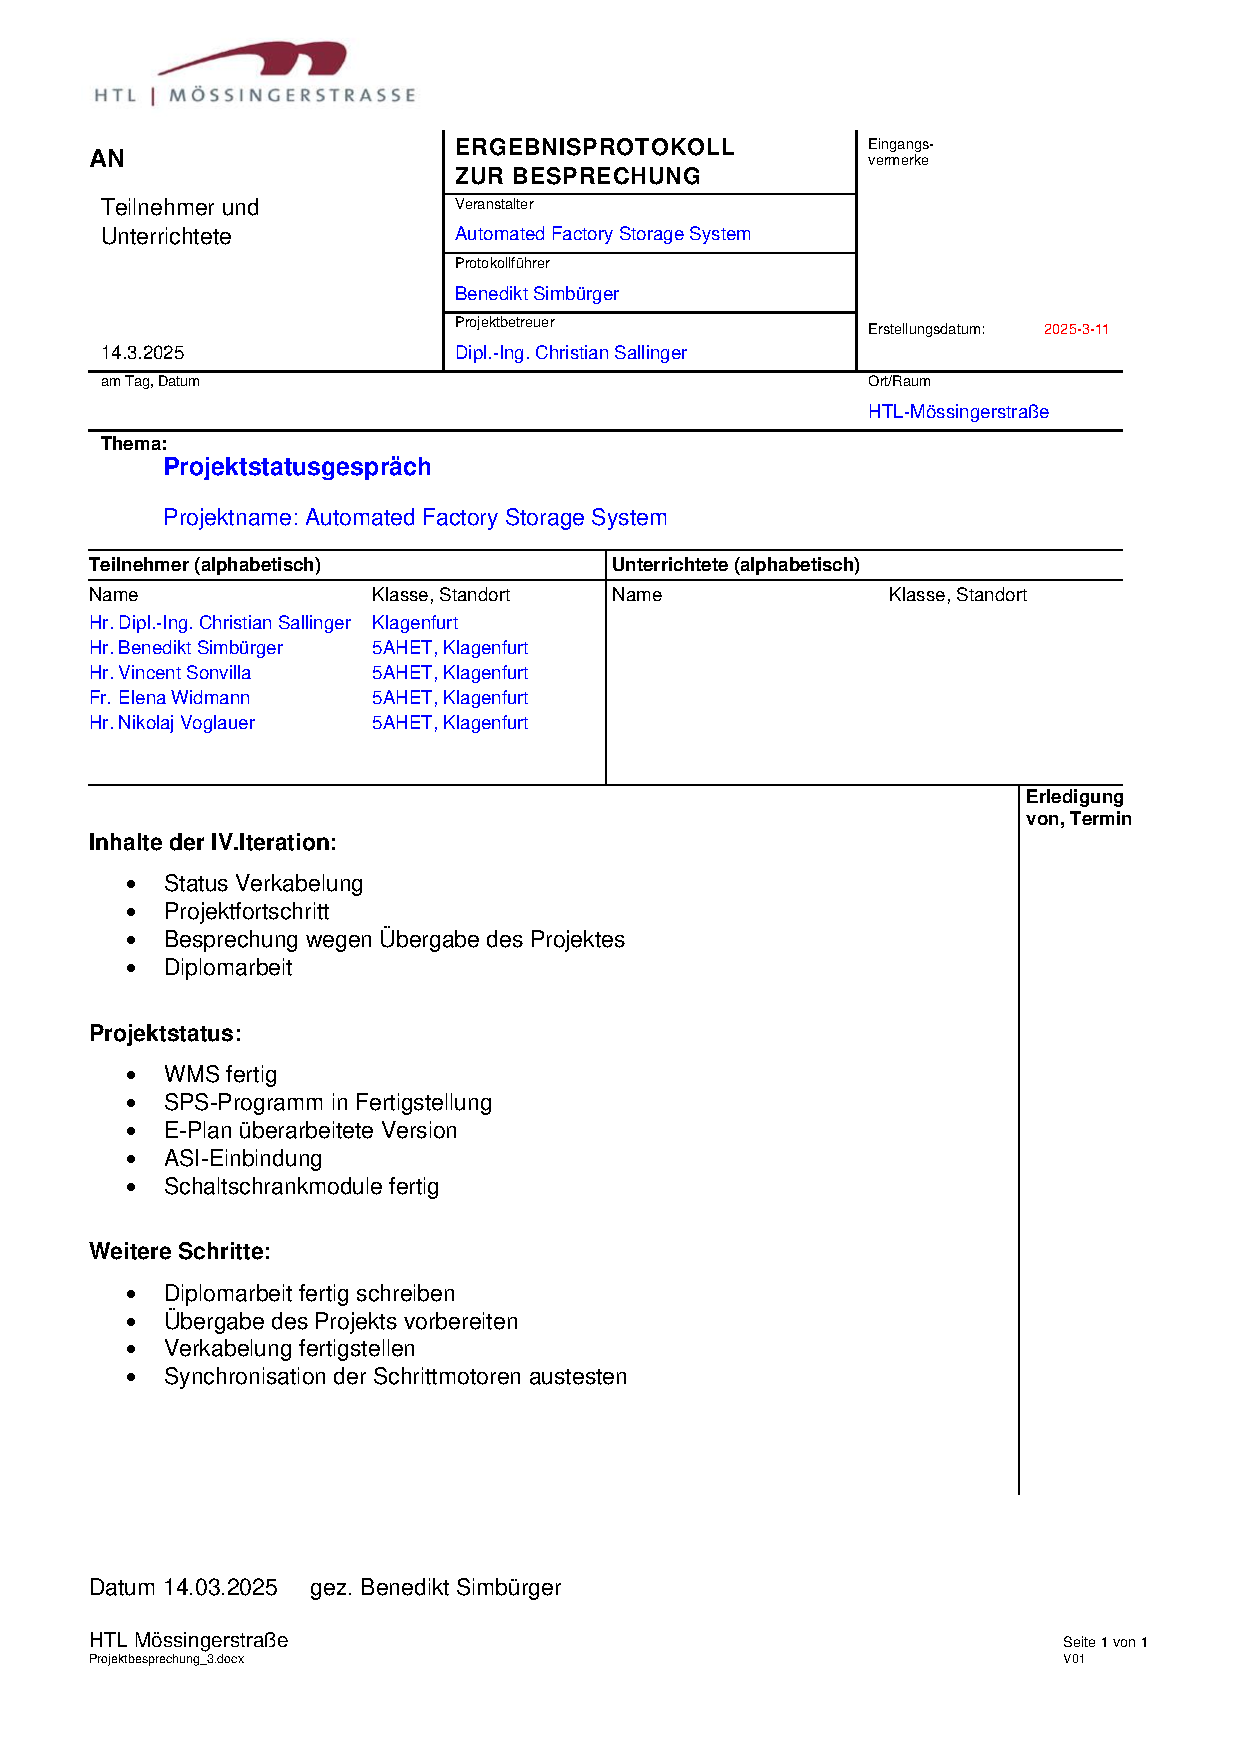
\includegraphics[width=0.9\textwidth]{../Protokolls/Projektbesprechung_3.pdf}
    \centering
    \caption{Besprechungsprotokoll x.x.xxxx}
\end{figure}




\newpage
\subsection{Arbeitsnachweis}

\subsubsection{Simbürger}

\begin{longtable}{|l|p{10cm}|r|}
    \hline
    \textbf{Datum} & \textbf{Tätigkeit} & \textbf{Stunden} \\
    \hline
    \endfirsthead

    \hline
    \textbf{Datum} & \textbf{Tätigkeit} & \textbf{Stunden} \\
    \hline
    \endhead

    \hline
    \endfoot

    \hline
    \endlastfoot

4.10.2023&Besprechung des weiteren vorgehens mit WB	&0.5\\
9.10.2023&Gruppenbesprechung für das weitere Vorgehen	&1.0\\

19.12.2023	&CAD Auf/Ab-fahrer	&3.0\\

10.1.2024	&Testversuch ET200 SPS Stepdrive und Meeting Knapp&	4.0\\
11.1.2024	&Achse mechanisch fertig, Schlitten vertikal&	4.0\\
12.1.2024	&CAD Schuttel, Tag der offenen Tür vorbereitung	&2.0\\
16.1.2024	&Motoren ansteuern&	1.0	\\
20.1.2024	&Umlenkungen- und Aufhängungskonstruktion&	4.0\\
29.1.2024	&Diagramm Datenaustausch Anfertigung&   2.0\\
1.2.2024	&Besprechung WB&	4.0\\
3.2.2024	&Website Backend/Frontend Prototyp&	9.0\\
4.2.2024	&WS Frontend&	3.0\\

5.2.2024	&KWF Antrag schreiben und WS Datenbankmanagement&	3.0\\
7.2.2024	&OPC UA Client testung&	4.5\\
15.2.2024	&WS Suche usw, Organisation, Maschinenbaubesprechung	&5.5\\

20.2.2024	&Python / OPC UA Client testen	&1.0\\
23.2.2024	&WS Warenkorb, restructuring	&9.0\\
24.2.2024	&WS Warenkorb fertig, OPC anfang und Pflichtenheft Erstversion&	6.0\\
27.2.2024	&http-Kommunikation	testen&4.0\\
28.2.2024	&Lasten/Pflichtenheft erstellen	&3.0\\
4.3.2024	&http-Kommunikation testen&	3.5\\
10.3.2024	&CAD X-Achse& 7.0\\
13.3.2024	&Absprache mit WB bez. Pflichtenheft	&1.0\\
14.3.2024	&http-Kommunikation und CAD&	3.0\\
1.4.2024	&Datenbanken und Visualisierung	&5.0\\
2.4.2024	&CAD Lagerregal&	2.0\\
17.4.2024	&CAD Gabel und Software&	2.0\\
23.4.2024	&STT-Fortsetzung / Software einführung&	2.5\\
12.4.2024	&Datenbanken und Visu	&5.0\\
21.4.2024	&Datenbanken und Visu	&5.0\\
22.4.2024	&TF-IDF Recherche	&3.0\\
23.4.2024	&TF-IDF Implementierung	&2.0\\
28.4.2024	&Areas und Locations Implementierung	&6.0\\
19.4.2024	&Order Algorithmus konzeptionieren	&3.0\\
22.5.2024	&Order Algorithmus Implementierung	&3.0\\
2.6.2024	&Order Api Programmierung	&5.0\\
3.6.2024	&Api Implementierung und Visu& 3.0\\
4.6.2024	&STT-Fortsetzung und CAD&	2.0\\
6.6.2024	&SPS/Server Communictaion und Z-Prototyp CAD	&5.0\\
8.6.2024	&SPS Comm und Simulation implement	&4.0\\
9.6.2024	&System Controller	&4.0\\

14.6.2024	&Z-Prototyp Bauteile Vorbereitung& 1.0\\
18.6.2024	&Return, Cart programmieren	&4.0\\
19.6.2024	&Docker (f me)	&3.0\\
21.6.2024	&Z-PT, Schaltschrank, SPS-Com&	4.5\\
16.7.2024	&Recherche, Referenz-Elektronik&	1.0\\
17.7.2024	&Ref-Elektronik	&2.0\\
19.7.2024	&Designe/CAD Rollen u. Spannen y &6.0\\
22.7.2024	&Design X-Spannelement	&2.0\\
25.7.2024	&Design X-Spannelement und Rollen	&1.5\\
31.7.2024	&CAD Z-Achsen zauberei &	1.0\\
1.8.2024	&CAD Z-Achse redesign & 5.0\\
9.8.2024	&CAD YZ-Achse grobe fertigstellung&	5.0\\
10.8.2024	&CAD YZ-Achse feinerschliff	&4.0\\
11.8.2024	&CAD YZ-Achse + X-Achse beginn&	2.0\\
12.8.2024	&CAD X-Achse	&1.0\\
13.8.2024	&CAD X-Achse side roller	&4.0\\
14.8.2024	&CAD X-Achse side roller 2. side	&2.0\\
15.8.2024	&CAD X-Achse Mid rollers, side Wheels, YZ-Achse Spiegelung	&6.0\\
16.8.2024	&CAD YZ-Achse Lichttaster, X-Achse	&1.0\\
17.8.2024	&X-Achse Schleppkettengedanken Auslegung	&6.0\\
19.8.2024	&Schleppenderketten einplanung	&2.0\\
20.8.2024	&CAD vertikale Schleppkette &3.0\\
20.8.2024	&Sponsoren-E-mail beginn	&1.3\\
21.8.2024	&Kontaktdaten, Projektzusammenfassung	&1.5\\
22.8.2024	&CAD Schlitten Top 	&1.0\\
24.8.2024	&Stückliste, CAD Schlitten Top	&2.0\\
25.8.2024	&CAD X-Top Verbindung, Umlenkung	&5.0\\
27.8.2024	&CAD Rahmen Aufhängungen	&2.0\\
29.8.2024	&CAD Umlenkungen und Motoraufhängungen	&5.0\\
30.8.2024	&CAD Endschalter und Rahmen beginn	&3.0\\
31.8.2024	&CAD Rahmen, Lagerschrank beginn	&6.0\\
1.9.2024	&CAD Lagerschrank und Querfördererausschnitt	&2.0\\
2.9.2024	&Verbidungsslider implementieren	&1.0\\
3.9.2024	&Bugs beheben, Weidmüller Sortiment Bauteile auswählen	&4.0\\
4.9.2024	&Stack Bug behoben und CAD Querförderer	&7.0\\
5.9.2024	&CAD Mech. weitestgehende Fertigstellung	&4.0\\
9.9.2024	&Latex aufsetzen	&2.5\\
10.9.2024	&Meeting Weidmüller&	2.0	\\
11.9.2024	&Schaltschrank konzeptionieren &2.25\\
15.9.2024	&Stückliste anfertigen	&2.0\\

17.9.2024	&Autolager Demontieren für Bauteilbeschaffung&	2.5\\
18.9.2024	&Verbindungstest, Suchalgorythmus Rust implementation &6.0\\
19.9.2024	&Suchag. Fertig implementiert, CAD Rollen gezeichnet	&3.0\\

24.9.2024	&Projektmanagement&	3.0\\
25.9.2024	&Änderungen V-Slot-Aufhängung, Project-Libre	&1.0\\

26.9.2024	&Igus, Weidmüller, Motoren ansteuern die 1.&	4.0\\
28.9.2024	&Bux im Lageralgorithmus beheben	&1.5\\

1.10.2024	&CAD	&1.0\\
3.10.2024	&Profile bearbeiten	&1.5\\
8.10.2024	&Latex Vorlage	&1.0\\
9.10.2024	&Raumeinrichtung&	3.0\\
21.10.2024	&Rahmenbau beginn&	2.0\\
22.10.2024	&Rahmenbau und Drehstromverlegung, Auftragsvorbereitung X-Aufhängung &5.5\\
23.10.2024	&Rahmenbau	&3.0\\
24.10.2024	&Rahmenbau	&3.0\\
25.10.2024	&CAD XZ-Redesign	&3.0	\\
26.10.2024	&CAD XZ-Redesign	&7.0	\\
27.10.2024	&Auftragsvorbereitung X-Achse	&3.0\\
28.10.2024	&Auftragsvorbereitung X-Achse	&2.0	\\

5.11.2024	&Beginn Umlenkrollen Drehen	&0.8\\
6.11.2024	&Weidmüller DP Inbetrtiebnahme&	1.0\\
7.11.2024	&Weidmülller DP ansteuern&	3.5\\
8.11.2024	&Weidmülller DP ansteuern&	3.5\\
12.11.2024	&Umlenkrollen Drehen &	3.5\\
19.11.2024	&Umlenkrollen Drehen, Fräsen	&2.5\\
20.11.2024	&DAS: Drehen	&1.0\\
21.11.2024	&DAS: TFIDF	&2.0\\
22.11.2024	&DAS	&4.5\\
23.11.2024	&API stack , DAS	&3.0\\
24.11.2024	&DAS	&2.0\\
25.11.2024	&DAS	&1.5\\

26.11.2024	&Drehen& 3.5\\
29.11.2024	&DAS& 4.0\\
3.12.2024	&Drehen, DAS: Maschinenbau& 5.0\\
6.12.2024	&Website, DAS &3.5\\
10.12.2024	&DAS: Software, CAD	&5.0\\
13.12.2024	&Drehen &3.5\\
7.1.2025	&CNC-Fräsen, Hülsen Drehen&	3.5\\
8.1.2025	&X-Achse Zusammenbauen anfangen	&2.0\\
10.1.2025	&X-Achse Zusammenbauen	&4.0\\
14.1.2025	&X-Achse Zusammenbauen &	4.0\\
15.1.2025	&X-Achse Zusammenbauen &	4.5\\
17.1.2025	&Tag der offenen Türe	&5.0\\
21.1.2025	&TIA Portal Verbindung&	3.5\\
24.1.2025	&Lasern, Förderband, Mechanik	&3.5\\
4.2.2025	&Sicherheitstechnik-Besprechung, SPS - Server Kommunikation	&3.5\\
14.2.2025	&WMS Location Updateing	&1.0\\
17.2.2025	&DAS: Allgemeinteil	&1.0\\
21.2.2025	&Ref, Fräsen, Da-Schreiben	&5.0\\
25.2.2025	&Zusammenbauen&	4.0\\
28.2.2025	&Fräsen, E-Plan,&	3.5\\
2.3.2025	&DAS: Aufbau	&1.5\\
3.3.2025	&DAS: Besprechungsprotokolle&	1.0\\
5.3.2025	&Umlenkung und Motoren einbauen&	4.5\\
6.5.2025	&DAS  &	2.5\\
9.3.2025	&DAS XZ-Achse	&1.0\\
10.3.2025	&DAS	&3.0\\
11.3.2025	&DAS	&3.0\\
14.3.2025	&Verkabelung Schaltschrank	&4.0\\
\end{longtable}
\newpage

\subsubsection{Sonvilla}
\begin{longtable}{|l|p{10cm}|r|}
    \hline
    \textbf{Datum} & \textbf{Tätigkeit} & \textbf{Stunden} \\
    \hline
    \endfirsthead

    \hline
    \textbf{Datum} & \textbf{Tätigkeit} & \textbf{Stunden} \\
    \hline
    \endhead

    \hline
    \endfoot

    \hline
    \endlastfoot

    4.10.2023	&	Besprechung des weiteren vorgehens mit WB	&	0.5 \\
    9.10.2023	&	Gruppenbesprechung für das weitere Vorgehen	&	1.0 \\
    29.11.2023	&	Lasern Schlitten	&	4.5 \\
    10.1.2024	&	Testversuch ET200 SPS Stepdrive inkl. Meeting Knapp	&	4.0 \\
    16.1.2024	&	Motor ansteuern	&	4.0 \\
    18.1.2024	&	Schritt-Motor ansteuern	&	4.0 \\
    19.1.2024	&	Schritt-Motor ansteuern	&	3.0 \\
    30.1.2024	&	Inventur/ Sortierung Knapp-Sponsoring	&	4.0 \\
    6.2.2024	&	Induktiver Sensor testen	&	1.5 \\
    7.2.2024	&	OPC UA Client	&	4.5 \\
    20.2.2024	&   OPC UA Client 	&	1.0 \\
    27.2.2024	&	Http-Kommunikation	&	4.0 \\
    13.3.2024	&	Absprache mit Wurnitsch bez. Pflichtenheft	&	2.0 \\
    14.3.2024	&	Http-Kommunikation	&	2.5 \\
    23.4.2024	&	STT-Fortsetzung 	&	2.0 \\
    25.4.2024	&	STT-Fortsetzung, Verkabelung	&	4.0 \\
    7.5.2024	&	STT-Fortsetzung,	&	1.5 \\
    14.6.2024	&	Z-Prototyp Bauteile Vorbereitung	&	1.0 \\
    21.6.2024	&	Z-PT, Schaltschrank, SPS-Com	&	4.5 \\
    10.9.2024	&	Meeting Weidmüller	&	1.3 \\
    17.9.2024	&	Autolager Demontieren für Bauteilbeschaffung	&	2.5 \\
    18.9.2024	&	Förderband Abmessen, Verbindungstest, Sensorensicherun	&	2.0 \\\\
    26.9.2024	&	Igus, Mororen ansteuern	&	3.0 \\
    3.10.2024	&	Profile bearbeiten	&	1.5\\
    4.10.2024	&	Sensoren testen	&	2.0\\
    9.10.2024	&	Raumeinrichtung	&	3.0\\
    15.10.2024	&	Profile bearbeiten	&	3.5\\
    21.10.2024	&	Rahmenbau beginn	&	2.0\\
    22.10.2024	&	Rahmenbauu + Drehstrom	&	3.5\\
    23.10.2024	&	Rahmenbau	&	3.5\\
    24.10.2024	&	Rahmenbau	&	3.5\\
    6.11.2024	&	Weidmüller DP Inbetriebnahme	&	3.5\\
    7.11.2024	&	Weidmülller ansteuern	&	3.5\\
    8.11.2024	&	Weidmülller ansteuern	&	3.5\\
    12.11.2024	&	Drehen	&	2.0\\
    15.11.2024	&	Fräsen	&	2.0\\
    19.11.2024	&	Drehen, Fräsen	&	1.5\\
    22.11.2024	&	SPS programmieren	&	3.5\\
    26.11.2024	&	SPS programmieren	&	3.5\\
    29.11.2024	&	Blockschaltbild, Diplomarbeit	&	3.5\\
    3.12.2024	&	Drehen, Diplomarbeit	&	3.5\\
    6.12.2024	&   Diplomarbeit	&	3.5\\
    10.12.2024	&	Diplomarbeit	&	3.5\\
    13.12.2024	&	E-Plan 	&	3.5\\
    7.1.2025	&	CNC-Fräsen	&	3.5\\
    10.1.2025	&	Rahmen Zusammenbau	&	4.5\\
    14.1.2025	&	Zusammenbau Rahmen, SPS	&	4.0\\
    15.1.2025	&	Zusammenbau Rahmen, Kabel verlegen	&	4.5\\
    17.1.2025	&	Tag der offenen Tür	&	6.5\\
    24.1.2025	&	Lasern, Förderband  &	3.5\\
    4.2.2025	&	SPS <--> Server	&	3.5\\
    21.2.2025	&   Fräsen	&	3.0\\
    25.2.2025	&	Zusammenbauen	&	4.0\\
    6.3.2025	&	DA-Schreiben	&	2.0\\
    11.3.2025	&	DA-schreiben	&	2.0\\
    14.3.2025	&	Verkabelung     &	4.0\\
    18.3.2025	&	Verkabelung	&	5.0\\
    19.3.2025   &   DA schreiben    &   2.0 \\
    22.3.2025   &   DA schreiben    &   5.0 \\
    23.3.2025   &   DA schreiben    &   2.0 \\
    25.3.2025	&	Synchronisation der Schrittmotoren	&	4.0\\
    26.3.2025   &   DA Schreiben    &   5.0 \\
    27.3.2025   &   DA Schreiben    &   3.0 \\
    28.3.2025	&	DA schreiben	&	3.0\\
\end{longtable}
\newpage

\subsubsection{Voglauer}
\begin{longtable}{|l|p{10cm}|r|}
    \hline
    \textbf{Datum} & \textbf{Tätigkeit} & \textbf{Stunden} \\
    \hline
    \endfirsthead

    \hline
    \textbf{Datum} & \textbf{Tätigkeit} & \textbf{Stunden} \\
    \hline
    \endhead

    \hline
    \endfoot

    \hline
    \endlastfoot 
    4.10.2023	&	Besprechung des weiteren vorgehens mit WB	&	0.5	\\
9.10.2023	&	Gruppenbesprechung für das weitere Vorgehen	&	1	\\
29.11.2023	&	RSTT Ausfahrer + Lasern Schlitten	&	3	\\
15.12.2023	&	Präsentation	&	1.5	\\
10.1.2024	&	Testversuch ET200 SPS Stepdrive inkl. Meeting Knapp	&	4	\\
12.1.2024	&	Handout für Elternverein	&	1.5	\\
16.1.2024	&	Motor ansteuern	&	3	\\
23.1.2024	&	Vorbereitung für Knapp-Besuch(HO)	&	2.5	\\
30.1.2024	&	Inventur/ Sortierung Knapp-Sponsoring	&	4	\\
1.2.2024	&	Besprechung WB	&	4	\\
15.2.2024	&	Besprechung Maschinenbau	&	1.5	\\
17.2.2024	&	Programmieren-weiterbildung(py)	&	3	\\
20.2.2024	&	el. Komponenten ausmessen 	&	2	\\
22.2.2024	&	Programmieren-weiterbildung(py)	&	1	\\
24.2.2024	&	Schaltschrank CAD	&	3.5	\\
24.2.2024	&	Pflichtenheft Erstversion	&	2	\\
27.2.2024	&	Barcode-Scanner/http-Kommunikation	&	4	\\
6.3.2024	&	Lasten/Pflichtenheft erstellen	&	1.25	\\
13.3.2024	&	Absprache mit Wurnitsch bez. Pflichtenheft	&	2	\\
14.3.2024	&	Barcode-Scanner/Fusion 360	&	3	\\
2.4.2024	&	Lagerregal-Planung	&	2	\\
23.4.2024	&	STT-Fortsetzung / Software einführung	&	2.5	\\
6.6.2024	&	SPS/Server Communictaion	&	3	\\
13.6.2024	&	Schaltschrank Konzeptionierung	&	2.25	\\
18.6.2024	&	Schaltschrank Konzeptionierung	&	2	\\
21.6.2024	&	Schaltschrank Konzeptionierung	&	4	\\
16.7.2024	&	CAD-Serverschrank Konstruktion Anfang Fusion	&	2	\\
18.7.2024	&	CAD-Serverschrank Konstruktion Montage-Schienen	&	2	\\
28.7.2024	&	CAD-Serverschrank finished	&	3	\\
6.8.2024	&	Schaltschrank Modul Konzeptionierung	&	1	\\
3.9.2024	&	Firmen anschreiben und Datei-Management	&	1	\\
9.9.2024	&	Marketing, Fortschritts-Leafletter	&	2.5	\\
10.9.2024	&	Meeting Weidmüller	&	0.5	\\
11.9.2024	&	Schaltschrank konzeptionierung 	&	2.25	\\
12.9.2024	&	Siemens und Lapp Anrufen+Schreiben	&	1	\\
15.9.2024	&	Schaltschrank Komponenten konstruieren	&	1,5	\\
17.9.2024	&	Presentation und Projektmanagement	&	3	\\
21.9.2024	&	el. Komponenten konstruieren sowie Profilschienen	&	2	\\
22.9.2024	&	el. Komponenten konstruieren + E-Plan Anfang	&	2	\\
24.9.2024	&	E-Plan Auffrischungsschulung / Project libre	&	2.5	\\
26.9.2024	&	Igus, Mororen ansteuern die 1.	&	1	\\
1.10.2024	&	Schaltschrank-Konzeptionierung, CAD-zeichnen	&	5	\\
4.10.2024	&	Schaltschrank-Konzeptionierung, CAD / E-plan - zeichnen	&	4	\\
6.10.2024	&	Schaltschrank-Konzeptionierung, CAD - zeichnen	&	0.5	\\
9.10.2024	&	Raumeinrichtung, Schaltschrank-Konzeptionierung	&	2,5	\\
15.10.2024	&	Schaltschrank-Konzeptionierung, E-Plan-zeichen	&	4	\\
22.10.2024	&	 2.Präsentation	&	1	\\
23.10.2024	&	Rahmenbau	&	1.5	\\
7.11.2024	&	E-Plan/Autocad	&	3.5	\\
8.11.2024	&	E-Plan/Autocad	&	3.5	\\
15.11.2024	&	E-Plan	&	3.5	\\
19.11.2024	&	Drehen, Fräsen	&	1.5	\\
22.11.2024	&	E-Plan	&	4,5	\\
26.11.2024	&	E-Plan	&	3.5	\\
29.11.2024	&	E-Plan	&	3.5	\\
6.12.2024	&	Website	&	2	\\
10.12.2024	&	ASI in E-Plan	&	3.5	\\
13.12.2024	&	E-Plan 	&	3.5	\\
7.1.2025	&	Schaltschrank E-Plan / CAD	&	3.5	\\
10.1.2025	&	CAD für Schaltschrankmodule	&	4.5	\\
14.1.2025	&	Zusammenbauen der Module	&	4	\\
15.1.2025	&	Kabel verlegen	&	2	\\
17.1.2025	&	Tag der offenen Türe	&	5	\\
21.1.2025	&	Schaltschrank Modifikationen	&	3.5	\\
23.1.2025	&	Schaltschrank Modifikationen / Module	&	0.5	\\
24.1.2025	&	 Förderband testen	&	2	\\
10.2.2025	&	DA schreiben	&	3.5	\\
12.2.2025	&	DA schreiben	&	2	\\
21.2.2025	&	Fräsen	&	2	\\
25.2.2025	&	Schaltschrank Zusammenbauen	&	3.5	\\
28.2.2025	&	Fräsen, E-Plan	&	3.5	\\
11.3.2025	&	DA-schreiben	&	3	\\
14.3.2025	&	Verkabelung	&	4	\\
17.3.2025	&	DA schreiben	&	3.5	\\
18.3.2025	&	Verkabelung	&	4	\\
19.3.2025	&	DA-schreiben 	&	2	\\
21.3.2025	&	Verkabelung	&	2.5	\\
26.3.2025	&	DA-Schreiben	&	2	\\
27.3.2025 &	DA-Schreiben	&	5	\\
\end{longtable}
\newpage




\newpage
\addcontentsline{toc}{section}{Literaturverzeichnis}
\printbibliography[title=Literaturverzeichnis]

\newpage
\renewcommand{\cftfigpresnum}{Abb. }
\setlength{\cftfignumwidth}{2cm}
\listoffigures

\newpage

\renewcommand{\cfttabpresnum}{Tab. }
\setlength{\cfttabnumwidth}{2cm}
\listoftables

\end{document}